\documentclass[11pt]{book}
\usepackage{amssymb,graphicx,amsmath,mathtools,float,subfig}
\usepackage{lscape}
\usepackage{listings}
\usepackage[utf8]{inputenc}
\usepackage[spanish, es-tabla]{babel}


% Chapters bonitos
\usepackage[Bjornstrup]{fncychap}
\usepackage{fancyhdr}
\pagestyle{fancy}
\fancyhf{}
\renewcommand{\headrulewidth}{0.5pt}
\fancyfoot[LE,RO]{\thepage}
\fancyhead[RO]{\slshape\nouppercase{\rightmark}}
\fancyhead[LE]{\slshape{\leftmark}}


% Tabular tras un section
\usepackage{indentfirst}	

% Links
\usepackage[linktocpage]{hyperref}
\hypersetup{
	colorlinks=false,
	citecolor=black,
	filecolor=black,
	linkcolor=red,
	urlcolor=black,
	pdfborderstyle={/S/U/W 1}
}


% Para cambiar el caption de las figuras
\usepackage[svgnames]{xcolor}
\definecolor{griscaption}{RGB}{100,100,100}
\usepackage{caption}
\usepackage[font={color=griscaption},figurename=Fig.,labelfont={bf}]{caption}

% Matemáticas
\newtheorem{theorem}{Teorema}
\newtheorem{corollary}[theorem]{Corolario}
\newtheorem{lemma}[theorem]{Lema}
\newtheorem{proposition}[theorem]{Proposición}
\newtheorem{definition}[theorem]{Definición}


% Fracciones más grandes
\newcommand\ddfrac[2]{\frac{\displaystyle #1}{\displaystyle #2}}

% Línea vertical para separar imágenes
\newcommand{\rulesep}{\unskip\ \vrule\ }

% Para solucionar el problema de títulos de secciones muy largos
\newcommand{\markedsection}[2]{\section[#2]{#2%
\sectionmark{#1}}
\sectionmark{#1}}

\newcommand{\markedchapter}[2]{\chapter[#2]{#2%
\chaptermark{#1}}
\chaptermark{#1}}


% Para llegar hasta subsubsection
\setcounter{tocdepth}{3}
\setcounter{secnumdepth}{3}



% Para el código
\definecolor{background}{rgb}{1.0, 0.96, 0.96}
\definecolor{emphasis}{rgb}{0.2,0.0,0.0}

\definecolor{gray97}{gray}{.97}
\definecolor{gray75}{gray}{.75}
\definecolor{gray45}{gray}{.45}
\definecolor{gray30}{gray}{.97}

\lstset{
	frame=Ltb,
	framerule=0.5pt,
	aboveskip=0.5cm,
	framextopmargin=3pt,
	framexbottommargin=3pt,
	framexleftmargin=0.1cm,
	framesep=0pt,
	rulesep=.4pt,
	rulesepcolor=\color{black},
	%
	stringstyle=\ttfamily,
	showstringspaces = false,
	basicstyle=\scriptsize\ttfamily,
	commentstyle=\color{gray45},
	keywordstyle={\color{emphasis}\bfseries},
	%
	numbers=left,
	numbersep=6pt,
	numberstyle=\tiny,
	numberfirstline = false,
	breaklines=true,
	literate={Ó}{{\'O}}1{í}{{\'i}}1{ó}{{\'o}}1,
	escapeinside={(*}{*)}
}

 
 
% Minimizar fragmentado de listados
\lstnewenvironment{listing}[1][]{\lstset{#1}\pagebreak[0]}{
	\pagebreak[0]
}

\lstdefinestyle{PythonCode}{
	basicstyle=\small,
	frame=single,
	backgroundcolor=\color{background},
	language=Python,
	numbers=left,
	emph={%  
		Para, cada, en, Desde, hasta, Si, Sino, Devuelve %
	},emphstyle={\color{emphasis}\bfseries}
}

 
\lstdefinestyle{Console}{
	basicstyle=\scriptsize\bf\ttfamily,
	backgroundcolor=\color{gray30},
	frame=single,
	numbers=none
}



\begin{document}
\begin{titlepage}
 
 
\newlength{\centeroffset}
\setlength{\centeroffset}{-0.5\oddsidemargin}
\addtolength{\centeroffset}{0.5\evensidemargin}
\thispagestyle{empty}

\noindent\hspace*{\centeroffset}

\begin{minipage}{\textwidth}
	\centering
	
\includegraphics[width=0.9\textwidth]{images/logo_ugr.jpg}\\[1.2cm]
	
	\textsc{\Large TRABAJO FIN DE GRADO\\[0.2cm]}
	\textsc{Doble Grado en Matemáticas e Ingeniería Informática}\\[0.8cm]
	% Upper part of the page
	% 
	% Title
	{\Huge\bfseries Determinación de Órbitas\\
	}
	\noindent\rule[-1ex]{\textwidth}{1pt}\\[2.5ex]
	{\large\bfseries El método de Laplace}
\end{minipage}

\vspace{1cm}

\noindent\hspace*{\centeroffset}

\begin{minipage}{\textwidth}
	\centering
	\textbf{Autor}\\ {Simón López Vico}\\[2.5ex]
	\textbf{Directores}\\ {Rafael Ortega Ríos\\Sergio Alonso Burgos}\\[1.5cm]
	
	
\includegraphics[width=0.3\textwidth]{images/logo_ciencias.png}
	\hspace{1.5cm}
	
\includegraphics[width=0.3\textwidth]{images/logo_etsiit.png}\\[0.1cm]
	\textsc{Facultad de Ciencias\\Escuela Técnica Superior de Ingenierías\\Informática y de Telecomunicación}\\
	\textsc{---}\\
	Granada, septiembre de 2020
\end{minipage}
%\addtolength{\textwidth}{\centeroffset}
%\vspace{\stretch{2}}
\newpage
\end{titlepage}




\thispagestyle{empty}
%\cleardoublepage

%\thispagestyle{empty}




\clearpage{\thispagestyle{empty}\cleardoublepage}

\thispagestyle{empty}
\begin{center}
{
	\large\bfseries Determinación de Órbitas Elípticas: el Método de Laplace
}\\
\end{center}

\begin{center}
	Simón López Vico\\
\end{center}

%\vspace{0.7cm}
\noindent{\textbf{Palabras clave}: elipse, mecánica celeste, determinación de órbitas, Laplace, derivación numérica, Python.}\\

\vspace{0.7cm}
\noindent{\textbf{Resumen}}\\

El estudio de métodos matemáticos para la determinación de la órbita de un cuerpo celeste con simples observaciones desde la Tierra es un tema que lleva desarrollándose desde que Newton presentara el primer método de determinación en 1687. Desde entonces han ido apareciendo nuevos y mejores procedimientos para obtener mayor precisión en la órbita, además de que la mejora en las tecnologías para la observación ha ayudado mucho a aumentar la eficacia de cada uno de estos métodos. Con todo esto, podemos conocer la posición en cualquier momento de un cuerpo celeste, lo que será importante para futuros viajes espaciales.\\

A lo largo de este trabajo, estudiaremos el método de determinación desarrollado por Laplace en 1780, que se bastará de únicamente tres observaciones de un objeto en la bóveda celeste en diferentes momentos para intentar aproximar de manera óptima su trayectoria alrededor del Sol.\\

Para empezar, introduciremos los principales conceptos de la mecánica celeste, así como la manera de realizar y medir las observaciones; esto será necesario a la hora de entender el método laplaciano. A continuación, veremos el método de Laplace, basado en aproximación numérica y resolución de ecuaciones, y el cálculo para la transformación de posición y velocidad a coordenadas astronómicas, que definirán la órbita del objeto por completo. Tras ello, se realizará un estudio sobre el número de soluciones que se pueden obtener utilizando el método de determinación y los cálculos para discernir entre cuál de todas las soluciones posibles es la válida.\\

Por último, se implementará un software capaz de aproximar una órbita mediante el método laplaciano para facilitar la aplicación de este, pues requiere de muchas operaciones. Por medio del programa desarrollado, se verán diferentes casos de aproximación con distintos cuerpos para así determinar la eficacia del método de Laplace estudiado.





\clearpage{\thispagestyle{empty}\cleardoublepage}




\thispagestyle{empty}
\begin{center}
{
	\large\bfseries Orbit Determination: Laplace's Method
}\\
\end{center}

\begin{center}
	Simón López Vico\\
\end{center}

%\vspace{0.7cm}
\noindent{\textbf{Keywords}: ellipse, celestial mechanics, orbit determination, Laplace, numerical differentation, Python.}\\

\vspace{0.7cm}
\noindent{\textbf{Abstract}}\\

The study of mathematical methods for determining the orbit of an astronomical object with simple observations from the Earth is a subject that has been developing since Newton presented the first method of determination in 1687. Ever since, new and better methods for obtaining greater accuracy in orbit have been developed, and improved technologies for observation have greatly helped to increase the effectiveness of each of these methods. With all this, we can determine the position of a celestial body at any time, which will be important for future space travel.\\

In this work, we will study the orbit determination method developed by Laplace in 1780, which, with only three observations of an object at three different times, will try to approximate optimally its movement around the Sun.\\

First, we will introduce the main concepts of celestial mechanics, as well as how to make and measure the observations; this will be necessary when understanding the Laplacian method. Next, we will see the Laplace method, based on numerical approximation and equation solving, and the calculation for the transformation of position and velocity into astronomical coordinates, which will define the object's orbit completely. After this, a study will be made on the number of solutions that can be obtained using the determination method and the calculations in order to discern between which among all the possible solutions is the valid one.\\

Finally, we will implement a software capable of approximating an orbit by means of the Laplacian method to facilitate its application, as many operations are required. By means of the program developed, different cases of approximation with different objects will be seen in order to determine the effectiveness of the Laplace method studied.

\newpage






\thispagestyle{empty}

\noindent\rule[-1ex]{\textwidth}{2pt}\\[4.5ex]

Yo, \textbf{Simón López Vico}, alumno de la titulación Doble Grado en Matemáticas e Ingeniería Informática de la \textbf{Facultad de Ciencias de la Universidad de Granada} y la \textbf{Escuela Técnica Superior de Ingenierías Informática y de Telecomunicación de la Universidad de Granada}, con DNI 26504148Y, autorizo la ubicación de la siguiente copia de mi Trabajo Fin de Grado en la biblioteca del centro para que pueda ser consultada por las personas que lo deseen.

\vspace{6cm}

\noindent Fdo: Simón López Vico

\vspace{2cm}

\begin{flushright}
Granada a 7 de septiembre de 2020.
\end{flushright}

\clearpage{\thispagestyle{empty}\cleardoublepage}

\thispagestyle{empty}

\noindent\rule[-1ex]{\textwidth}{2pt}\\[4.5ex]

D. \textbf{Rafael Ortega Ríos}, Profesor del Departamento de Matemática Aplicada de la Universidad de Granada.

\vspace{0.5cm}

D. \textbf{Sergio Alonso Burgos}, Profesor del Departamento de Lenguajes y Sistemas Informáticos de la Universidad de Granada.


\vspace{0.5cm}

\textbf{Informan:}

\vspace{0.5cm}

Que el presente trabajo, titulado \textit{\textbf{Determinación de Órbitas Elípticas: el Método de Laplace}}, ha sido realizado bajo su supervisión por \textbf{Simón López Vico}, y autorizamos la defensa de dicho trabajo ante el tribunal que corresponda.

\vspace{0.5cm}

Y para que conste, expiden y firman el presente informe en Granada a 7 de septiembre de 2020.

\vspace{1cm}

\textbf{Los tutores:}

\vspace{5cm}

\noindent \textbf{Rafael Ortega Ríos \ \ \ \ \ Sergio Alonso Burgos}


\clearpage{\thispagestyle{empty}\cleardoublepage}

\thispagestyle{empty}


\begin{Huge}
\textbf{Agradecimientos}
\end{Huge}
\thispagestyle{empty}

\vspace{1cm}

Gracias a mis tutores, por toda la ayuda que me han brindado durante todos estos meses de pandemia, a pesar de todas las dificultades del camino. A Rafael Ortega Ríos por descubrirme la mecánica celeste y hacer que me guste aún más el estudio del universo que nos rodea, y a Sergio Alonso Burgos por su atención y ayuda para todo el desarrollo informático.\\

Pero en especial, gracias a mi familia, por soportar todos los momentos de agobio durante estos años de estudio y ayudarme a seguir adelante. La cuesta arriba se hubiera hecho más difícil sin vuestra ayuda, gracias de corazón.

\clearpage{\thispagestyle{empty}\cleardoublepage}

\thispagestyle{empty}



\thispagestyle{empty}
\pagenumbering{roman} % Start roman numbering
%\begingroup
	%\newpage
	%\let\cleardoublepage\relax
	%\let\clearpage\relax
	\tableofcontents  % para generar el índice de contenidos
	\thispagestyle{empty}
	\listoffigures    % para generar el índice de las imágenes
	\thispagestyle{empty}
	%\newpage
%\endgroup



\chapter{Introducción}
\label{chap:introduction}
En este trabajo nos vamos a centrar en el problema de determinación de órbitas, que consiste en determinar los elementos orbitales de un cuerpo a partir de $N$ observaciones realizadas desde la Tierra y así poder situar dicho objeto en la bóveda celeste en cualquier momento. Concretamente, se estudiará el método de determinación Laplaciano, el cuál fue desarrollado en 1780 y que sirvió como base para los métodos que fueron apareciendo posteriormente.	Dado que vamos a trabajar con observaciones tomadas desde la Tierra, no conoceremos una parametrización del movimiento real del cuerpo cuya órbita determinar y por tanto nos serviremos del cálculo numérico con el fin de aproximar las cantidades que necesitemos para nuestro trabajo. Además, haremos un repaso de la mecánica celeste comentando los principales elementos que necesitaremos para nuestro estudio de determinación.\\

Una vez estudiado el método de Laplace, discutiremos el número de soluciones del problema que podemos obtener, buscando asegurar la unicidad y teniendo en cuenta que no todas las soluciones son válidas para nuestro problema físico. Por último, se desarrollará un programa que sea capaz de calcular la órbita de un cuerpo a partir de los datos introducidos de sus observaciones desde la Tierra, facilitando así la aplicación del método de Laplace.\\

El trabajo desarrollado en esta memoria está basado principalmente en el estudio de ``\textit{An Introduction to Celestial Mechanics}'', escrito por Forest Ray Moulton \cite{moulton}, así como en ``\textit{Introducción a la Mecánica Celeste}'' de Rafael Ortega Ríos y Antonio Jesús Ureña Alcázar \cite{ortega} y en los conocimientos adquiridos durante la carrera de cálculo numérico \cite{MNII}. Todas las imágenes utilizadas han sido construidas utilizando la herramienta online que proporciona el software matemático Geogebra \cite{geogebra} o generadas a través del programa implementado. Para el desarrollo informático se ha utilizado el lenguaje de programación Python, estudiado durante la carrera, junto a diferentes paquetes facilitados por el mismo lenguaje, y nos ha sido de gran ayuda la efemérides proporcionada por Jet Propulsion Laboratory (JPL) \cite{jpl}.\\

Pero, antes de entrar de lleno en las matemáticas, veamos un poco de historia sobre la determinación de órbitas.\\


\section{Una breve historia de la determinación de órbitas.}
\label{sec:history}
En 1687, Isaac Newton publica la primera edición de su obra \textit{Philosophiæ Naturalis Principia Mathematica}, más comúnmente llamado \textit{Principia}, dando el primer método de determinación de órbitas mediante tres observaciones, concretamente de órbitas parabólicas. Dicho método dependía de una construcción gráfica y una serie de aproximaciones sucesivas. Años más tarde, en 1705, Edmund Halley utilizó dicho método para calcular la órbita del cometa que lleva su mismo nombre, junto a otros cuerpos \cite{moulton}.\\

El primer método que apareció el cuál no dependía de una construcción gráfica fue dado en 1744 por Leonhard Euler. Aún así, hasta este momento los métodos estaban basados en mayor parte en suposiciones no del todo ciertas, por lo que Johann Heinrich Lambert intenta eliminar estas suposiciones y extiende el trabajo de Euler. Además, estudia la determinación para órbitas hiperbólicas y elípticas.\\

Durante años se siguen estudiando y desarrollando estos métodos, hasta que en 1780 Pierre-Simon Laplace publica un método completamente nuevo, el cual estudiamos en este trabajo, que se convierte en la base para muchos trabajos posteriores.\\

En el año 1801, Giuseppe Piazzi observa por primera vez el planeta enano Ceres durante un mes, obteniendo unas 20 observaciones de éste, aunque pronto se pierde su pista. Este hecho llama la atención al matemático Carl Friedrich Gauss, que comienza a desarrollar un método para encontrar los elementos orbitales de un objeto a partir de simples observaciones hechas desde la Tierra. Rápidamente Gauss resuelve el problema y un año más tarde H. W. Olbers y F. Von Zach, aplicando el método desarrollado, recuperan la órbita de Ceres ayudando a situar el cuerpo en la bóveda celeste de nuevo. Al igual que con el método de Laplace, este trabajo se convierte en un pilar para la determinación de órbitas. \cite{moulton}\\


Todos estos métodos son de hace siglos, por lo que la tecnología en ese entonces era muy limitada y las observaciones eran hechas con telescopios ópticos, tomando dos ángulos para situar el cuerpo observado pero sin poder conocer a priori la distancia del objeto. Actualmente, además de telescopios ópticos (mucho más avanzados que los que usaban Gauss o Laplace) se utilizan telescopios radar, y realizando las observaciones con estos dos tipos de telescopio en conjunto podemos conseguir la posición del objeto que observamos con mucha precisión, e incluso conocer la distancia y velocidad de éste gracias a los telescopios radar \cite{brett_r_wilson} \cite{vetter}. Esta mejora en las tecnologías de observación ha causado que se desarrollen nuevos problemas de determinación, en su mayor parte debido a la ingente cantidad de datos que se pueden obtener. \cite{gronchi}\\

La determinación de órbitas es un campo de estudio que tiene continuidad y actualmente sigue en uso, aunque con métodos mucho más modernos que el que desarrollaremos en este trabajo \cite{gronchi_unesco}. Uno de sus usos es para cartografiar el cinturón de asteroides, trabajo que (aparte de ser bonito) será muy importante en un futuro cuando comience la navegación espacial.\\


\section{Familiarizándonos con el problema.}
Como hemos comentado anteriormente, el método de Laplace fue desarrollado en el siglo XVIII, por lo que la instrumentación para la observación era limitada y surge una dificultad: observando un cuerpo desde la Tierra, la cuál se encuentra en continuo movimiento, podremos obtener la dirección del objeto percibida por el observador, sin ninguna información sobre su distancia. Al no disponer de esta distancia no podremos determinar su posición exacta, por lo que las componentes de la velocidad no podrán ser calculadas. Así, habremos de tomar observaciones complementarias. Pero, ¿cuántas necesitaremos, como poco, para obtener todos los elementos de la órbita?\\

A lo largo de esta memoria veremos que una órbita se define por seis elementos, por lo que nos bastará con que las observaciones nos proporcionen al menos seis valores independientes entre ellos. A partir de una observación completa obtenemos dos cantidades, referentes a las coordenadas angulares del cuerpo observado; por lo tanto, serán suficientes tres observaciones del objeto a determinar su órbita para comenzar nuestro proceso. Por otra parte, hay que tener en cuenta que, previo a nuestro estudio, podemos conocer algunos elementos de la órbita. Por ejemplo, si la órbita es parabólica\footnote{En este trabajo no se tratan las órbitas parabólicas de los objetos observados, y este ejemplo solo es ilustrativo de cómo podríamos utilizar menos de 3 observaciones completas a la hora de realizar la determinación de la órbita.}, conocemos su excentricidad ($e=1$), por lo que no serán necesarios seis elementos, sino cinco, y de esta manera una de las observaciones realizada puede ser dejada a medias, proporcionando solo una de las coordenadas angulares.\\

Las coordenadas angulares del cuerpo que observemos serán obtenidas en ascensión recta y declinación, un método de medida similar a la latitud y longitud utilizada sobre la superficie de la Tierra. Utilizaremos dichas coordenadas ya que la posición del cuerpo será determinada midiendo las distancias angulares y direcciones respecto a las estrellas vecinas, que se suponen fijas y están catalogadas en este tipo de coordenadas. Aún así, podremos cambiar a cualquier otro tipo de sistema de coordenadas cuando lo requiramos.\\

Comencemos viendo cuáles son los distintos elementos de una órbita, así como qué es la ascensión recta y declinación, que en conjunto llamaremos coordenadas ecuatoriales.\\





\section{Elementos Orbitales y Coordenadas Ecuatoriales}
\label{sec:orbital_elements_equatorial_coordinates}
En este apartado realizaremos un repaso a la mecánica celeste (objetivo 1), estudiando los diferentes parámetros que identifican una órbita (de manera única) así como las coordenadas ecuatoriales, elementos que forman un sistema que nos permite ubicar el objeto observado respecto al ecuador celeste y al equinoccio vernal (que definiremos más adelante) en un momento preciso.\\

\subsection{Elementos Orbitales}
\label{subsec:orbital_elements}
Comencemos por los elementos orbitales, los cuales necesitarán sostenerse en las dos primeras leyes de Kepler para ser desarrollados. Dichas leyes son:

\begin{enumerate}
\item \textit{Todos los planetas se desplazan alrededor del Sol describiendo órbitas elípticas, con el Sol en uno de los focos de dicha elipse.}
\item \textit{Cada objeto barre áreas iguales en tiempos iguales.}
\end{enumerate}

Pues bien, con esto comencemos a desarrollar nuestros elementos, entendiendo qué es una elipse y como se comporta matemáticamente.
\begin{definition}
La elipse es una curva plana, simple y cerrada, que consta de dos focos (puntos fijos) de manera que para cualquier punto de la curva que tomemos, la suma de las distancias de los focos a dicho punto es la misma. \cite{ortega}
\end{definition}

Llamando a nuestra elipse $E$ y a los focos de ésta $F_1$ y $F_2$, podemos escribir la definición superior de la siguiente manera:
\[
|x-F_1|+|x-F_2|=d, \; \forall x \in E \implies d>|F_1-F_2|
\]

Notar que en el caso de que $d=|F_1-F_2|$ estaremos ante un segmento que unirá los focos, mientras que si $0=|F_1-F_2|$, es decir, los dos focos son el mismo, nos encontraremos con que nuestra curva es una esfera.\\

Tomando uno de los focos como el origen de nuestro sistema de coordenadas, comencemos a desarrollar las ecuaciones anteriores. Sea $x$ un punto de la elipse, tenemos:
\[
|x|-|x-F|=d \implies |x-F|=d-|x| \implies |x-F|^2=(d-|x|)^2\\
\]

Como estamos trabajando con vectores, tenemos que $|x-y|^2=|x|^2+|y|^2-2\langle x,y\rangle$, denotando con $\langle\cdot,\cdot\rangle$ el producto escalar de dos vectores. Por tanto, continuando el resultado anterior:
\[
|F|^2-2\langle x,F\rangle=d^2+2d|x| \implies |x|-\frac{\langle x,F\rangle}{d}=\frac{d^2-|F|^2}{2d}
\]

Definimos así los valores $k\in\mathbb{R}$, que se corresponde con el factor de la derecha, $k=\frac{d^2-|F|^2}{d}$, y $\vec{e}\in\mathbb{R}^2$, $\vec{e}=-\frac{1}{d}F$. Por la desigualdad triangular, $|F|<|x|+|x-F|=d$, obtenemos que $|\vec{e}|<1$ y $k>0$. Por tanto, llegamos a la ecuación:
\begin{align}
|x|+\langle \vec{e},x\rangle=k,
\label{eq:elipse_cartesiana}
\end{align}

\noindent que será la ecuación que describe todas las elipses con un foco en el origen \cite{mecanica_celeste}.\\

\begin{figure}[H]
\centering
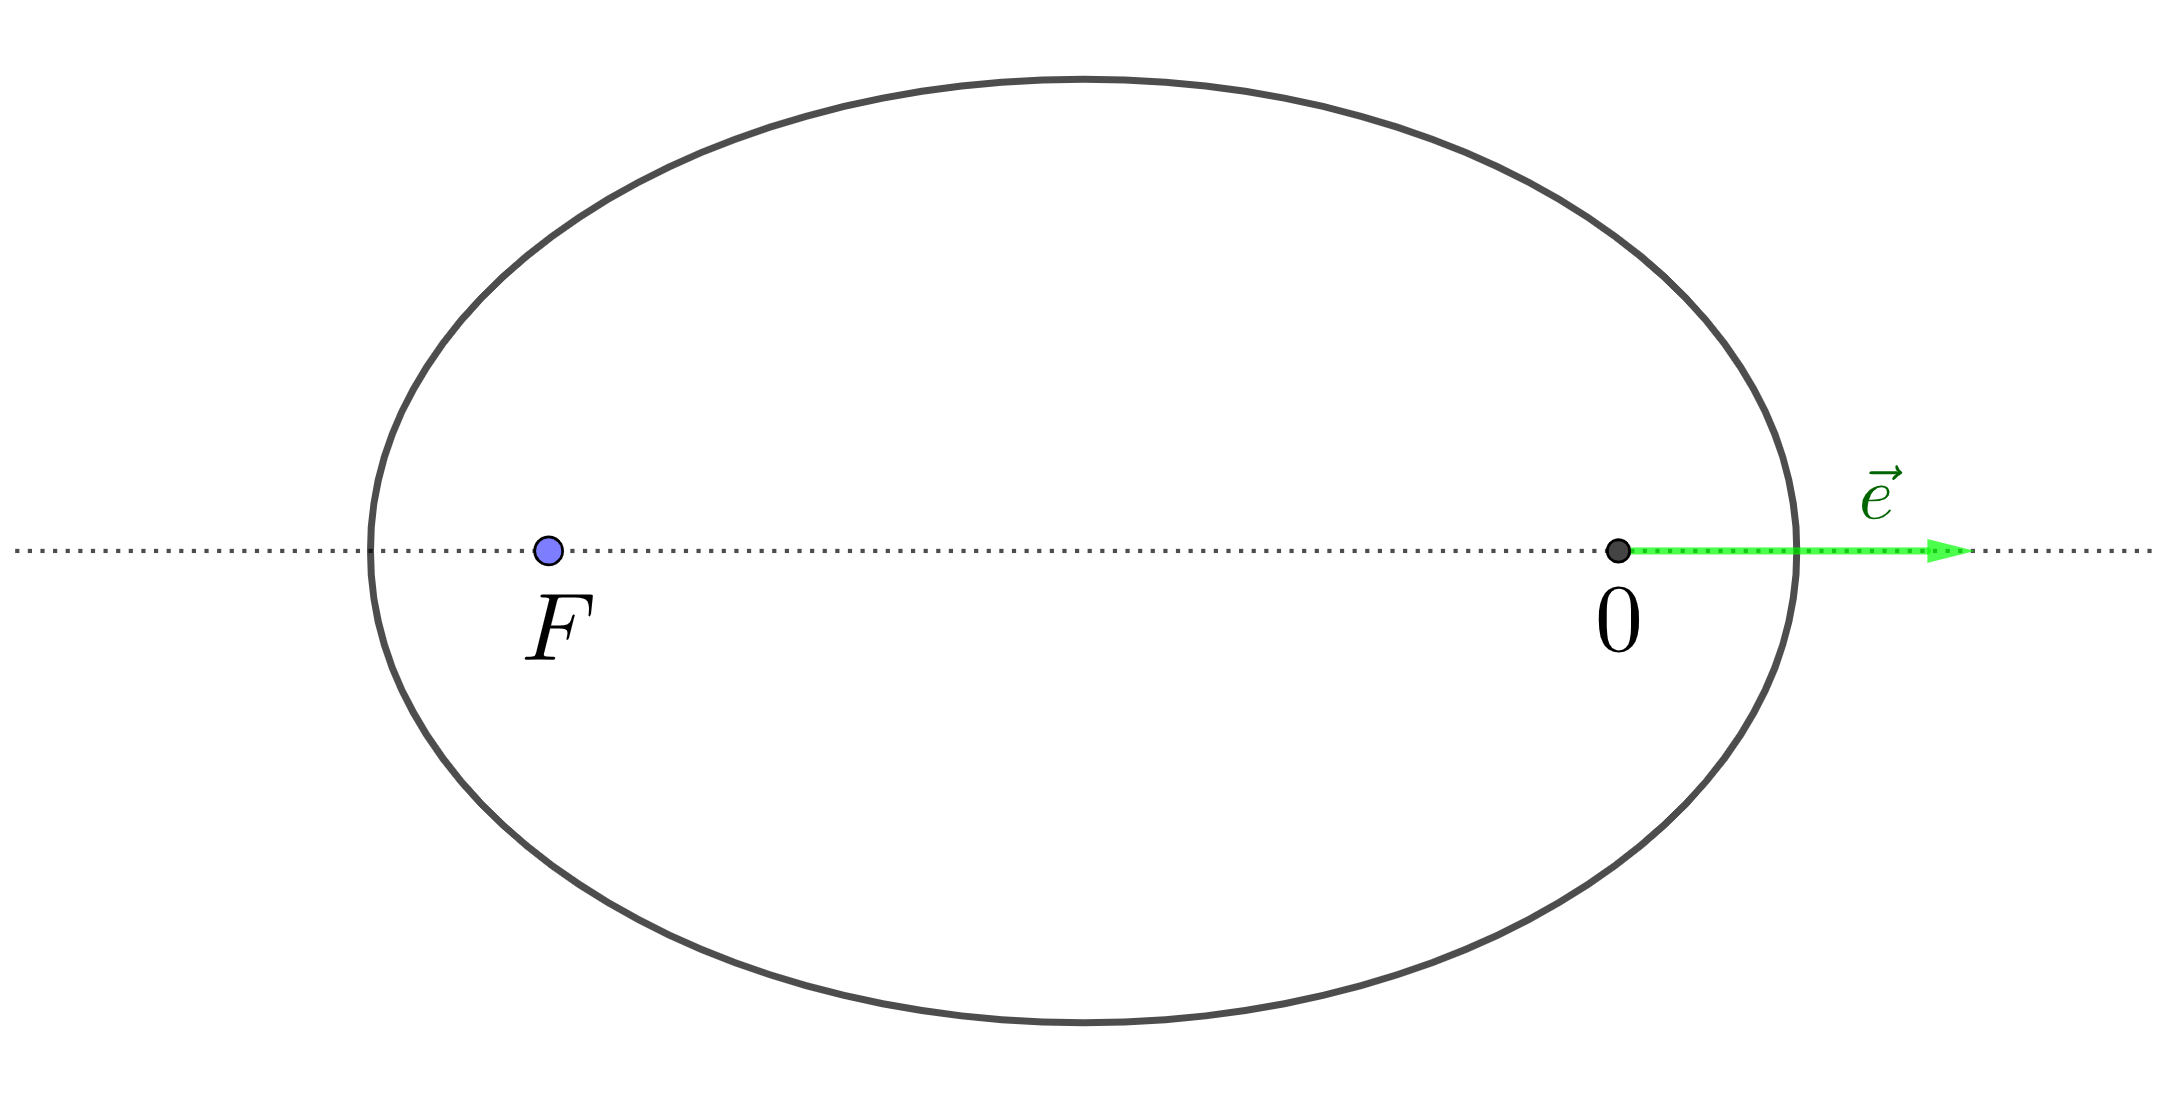
\includegraphics[scale=0.12]{images/elipse_excentricidad.png}
\caption{Representación de una elipse junto a sus focos y el vector $\vec{e}$.}
\label{fig:elipse_excentricidad}
\end{figure}

Llamaremos a $|\vec{e}|=e$ la \textbf{excentricidad de la elipse}, tomando valores en $[0,1[$. A mayor valor de excentricidad, mayor separación entre los focos, y viceversa. Si el valor de $e$ es 0, la curva que trazará el objeto será circular, los dos focos son iguales. Fuera del intervalo donde hemos definido la excentricidad, si $e=1$ la órbita del objeto es una parábola, y si es mayor que 1, el objeto describirá una órbita hiperbólica, aunque estos conceptos no serán necesarios para nuestro estudio de determinación.\\

Si trazamos una recta que pase por los dos focos de nuestra elipse, como podemos ver en \hyperref[fig:elipse_excentricidad]{la figura \ref{fig:elipse_excentricidad}}, dicha recta se intersecará con la elipse, obteniendo así dos puntos a los que llamaremos perihelio ($P$, más cercano a $0$) y afelio ($A$, más cercano a $F$). Si tomamos el centro de la elipse como el punto medio entre los dos focos y medimos la distancia desde el centro hasta el perihelio (o, equivalentemente, hasta el afelio), obtendremos el \textbf{semieje mayor} de la elipse, al que notaremos por $a$. Por otra parte, si trazamos una perpendicular a la recta que pasa por los focos que pase por el centro de la elipse, la distancia desde una de las intersecciones con la elipse hasta el centro nos dará el semieje menor, al que representaremos por $b$ \cite{ortega}. Podemos entender más fácilmente estos valores en la siguiente figura.

\begin{figure}[H]
\centering
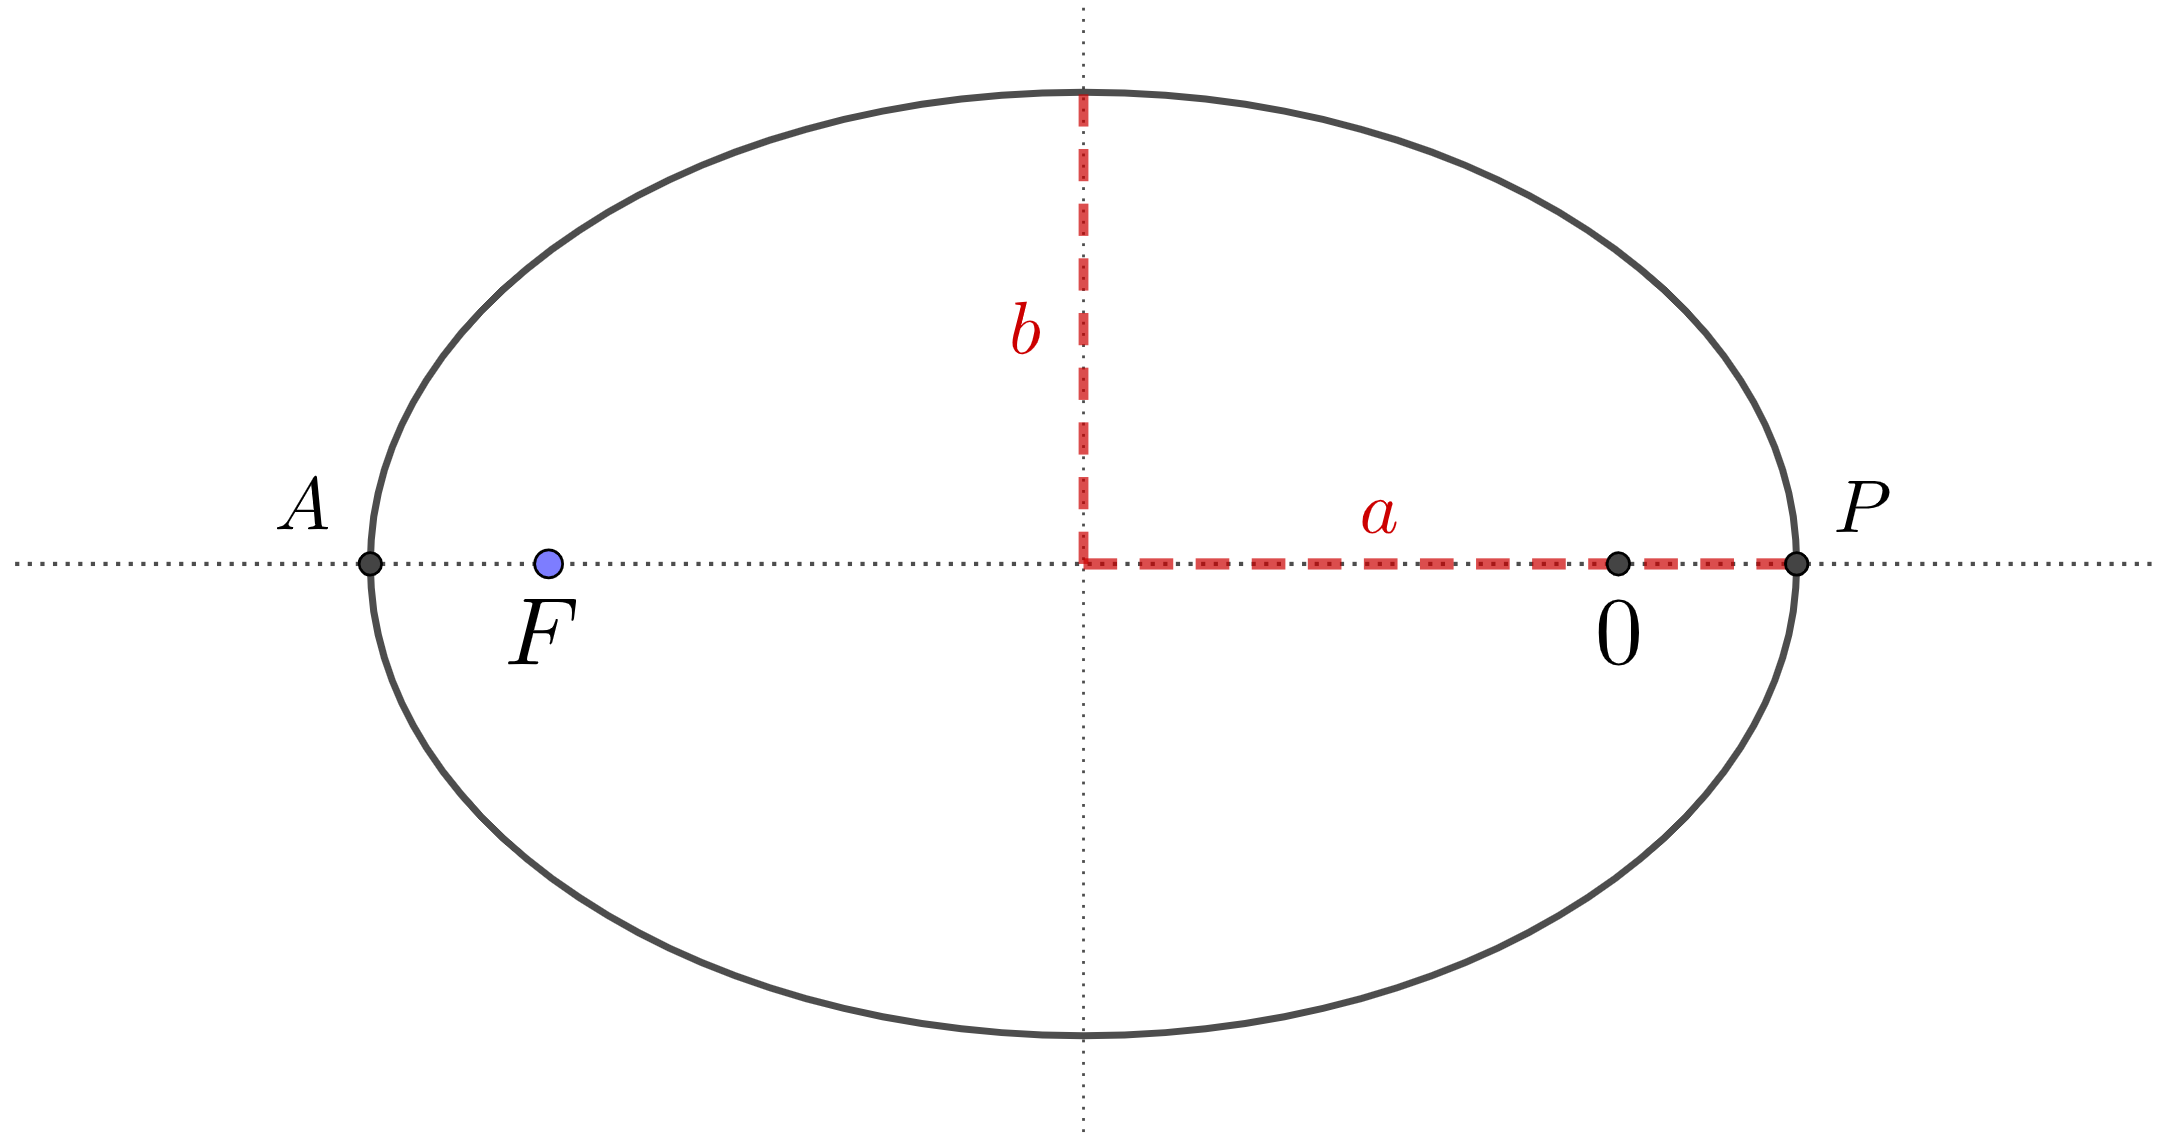
\includegraphics[scale=0.12]{images/perihelio_afelio.png}
\caption{Elementos geométricos de la elipse.}
\label{fig:perihelio_afelio}
\end{figure}


Notemos dos relaciones interesantes entre los elementos de la elipse comentados anteriormente y su excentridad:
\[
\frac{b}{a}=\sqrt{1-e^2}, \; \; \; \; \; \; \; \; \; \; \; \; \; \; \; \; \; \; \; \; e=\frac{\text{distancia entre los focos}}{\text{eje mayor}}=\frac{\overline{OF}}{2a}
\]

El punto donde se intersecan el semieje mayor y menor será el centro de la elipse, $C$, y podremos obtener una expresión de la distancia de cada uno de los focos a éste a partir de la segunda ecuación superior, sabiendo así que $\overline{0C}=\overline{FC}=ae$.\\

Por último, notemos por $\omega\in\mathbb{R}/2\pi\mathbb{Z}$ al \textbf{argumento del periastro}\footnote{El periastro toma diferentes nombres en función de qué objeto ocupe el foco 0, por ejemplo, si en dicho foco se encuentra el Sol lo llamaremos perihelio, si se encuentra la Tierra el perigeo, etc.}, que representará el ángulo formado entre el eje polar (equivalente al eje $x$ en el sistema cartesiano) y la dirección del vector $\vec{e}$. Así, tenemos que:
\[
\vec{e}=e(\cos{\omega},\sin{\omega})
\]

Llamemos $\mathcal{E}_0$ al espacio de elipses con foco en el origen, donde cada elipse queda determinada de manera única por su \hyperref[eq:elipse_cartesiana]{ecuación cartesiana}. Los parámetros $a$, $e$ y $\omega$ dan lugar a sistema de coordenadas en $\mathcal{E}_0$, que está definido sobre $\mathbb{R}^2$. Aquí surge un problema, pues las órbitas de los planetas son elipses en el espacio, cada una situada en un plano distinto, con un sentido de giro. Por tanto, será necesario definir un nuevo conjunto de parámetros para obtener un sistema de coordenadas sobre tres dimensiones.\\

Para empezar, definamos un sistema de referencia ortonormal en el espacio, que situará al Sol en el origen, y el plano $z=0$, en el que se encontrará el recorrido de la órbita de la Tierra, llamado plano de la eclíptica.\\

Empezamos definiendo el vector unitario $\vec{e}_3$, el cuál fijaremos como el normal al plano de la eclíptica. Dado que hay dos opciones (el normal positivo y el normal negativo), lo fijaremos a partir de la orientación que da el eje terráqueo de Sur a Norte. A continuación definimos $\vec{e}_1$, que tomamos en la recta formada por la intersección del plano del ecuador celeste con el plano de la eclíptica y dirección el punto vernal, situado en la constelación de Piscis\footnote{Antiguamente al punto vernal se le llamaba punto Aries debido a que la constelación a la que apuntaba era la constelación de Aries, pero durante los años dicho punto ha ido desplazándose hasta encontrarse apuntando a Piscis \cite{piscis}.}. Para terminar, escogemos el vector $\vec{e}_2$ como el vector ortonormal a $\vec{e}_1$ que está también en el plano de la eclíptica. Como de nuevo hay dos opciones, tomaremos el que de sentido positivo al giro de la Tierra (giro antihorario).\\

\begin{figure}[H]
\centering
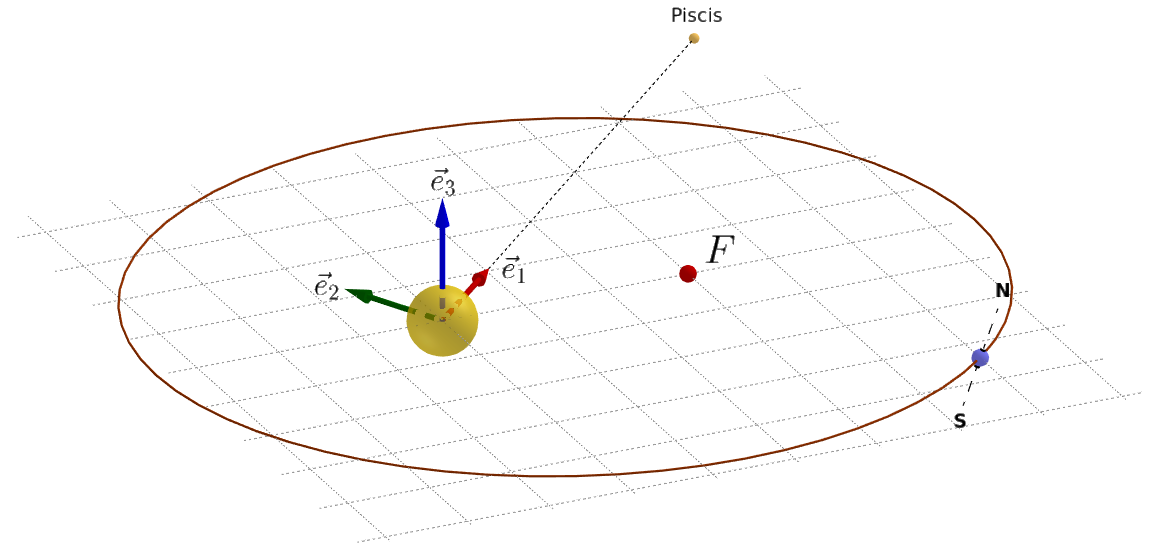
\includegraphics[scale=0.3]{images/sistema_coordenadas.png}
\caption{Órbita elíptica de la Tierra con focos $F$ y el Sol, mostrando el sistema de referencia. En la órbita terrestre real, el foco $F$ se encuentra dentro del Sol.}
\label{fig:sistema_referencia}
\end{figure}

Así, tenemos un sistema ortonormal $\{\vec{e}_1,\vec{e}_2,\vec{e}_3\}$ de manera que la orientación del movimiento de la Tierra se corresponde con la orientación $\{\vec{e}_1,\vec{e}_2\}$ del plano de la eclíptica \cite{mecanica_celeste}.\\

Para determinar una órbita elíptica por completo necesitaremos cinco elementos; $a$, $e$ y $\omega$ definidos anteriormente, y dos más que introduciremos a continuación que definirán el plano de movimiento: la \textbf{inclinación} respecto al plano de la eclíptica ($i$) y el \textbf{argumento del nodo ascendente} ($\Omega$).\\

Fijemos la línea de nodos como la recta que interseca el plano de movimiento del objeto observado y el plano de la eclíptica; sean $\vec{n}$ el vector normal al plano de movimiento, que es unitario y su sentido es el del momento angular, y $\mathcal{N}_+$ el lado positivo de la línea de nodos. Entonces:
\[
\left\{
\begin{array}{l}
	i=\measuredangle(\vec{e}_3,\vec{n}), \; \; \; \; \; \; \; \; \; \; i\in]0,\pi[\\
	\Omega=\measuredangle(\vec{e}_1, \mathcal{N}_+), \; \; \; \; \; \Omega\in\mathbb{R}/2\pi\mathbb{Z}
\end{array}
\right.
\]\\

Una vez hayamos definido el plano de movimiento con estos dos valores, encontramos la elipse usando la línea de nodos como eje de rotación para el argumento del perihelio, $\omega$.

\begin{figure}[H]
\centering
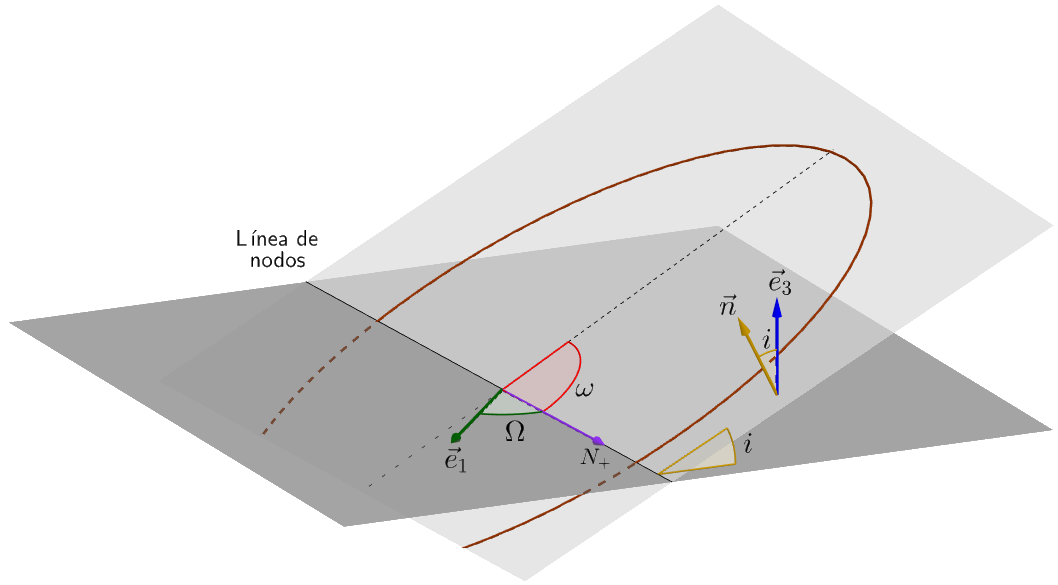
\includegraphics[scale=0.34]{images/omega_i.png}
\caption{Plano de movimiento del cuerpo definido por sus elementos orbitales.}
\label{fig:omega_i}
\end{figure}

Al conjunto de estas cinco coordenadas lo llamaremos \textbf{Coordenadas Astronómicas} o elementos orbitales, y están bien definidas y son unívocas en la región $i\in]0,\pi[$, $e\in]0,1[$, excluyendo así las órbitas circulares y las definidas sobre el plano de la eclíptica \cite{ortega}.\\

A estas cinco coordenadas podremos añadirle una sexta que por medio de la ecuación de Kepler nos permita determinar la posición del planeta para un momento $t$. Ese sexto elemento puede ser el valor $T$, que se define como el momento de paso por el perihelio, la fecha concreta del momento en el que el objeto está en el perihelio de su órbita. También puede ser usada la anomalía media, $M=n(t-T)$, con $n=\frac{2\pi}{p}$ el movimiento medio y $p$ el período de la órbita. Ésta representa la fracción del período de una órbita que transcurre desde que el cuerpo pasa por el perihelio hasta el momento $t$; obteniendo este ángulo podemos situar el objeto en el punto exacto de la órbita en el que se encuentra \cite{ortega}.\\

Cuando añadamos un sexto elemento a las coordenadas astronómicas tendremos que señalar una diferencia: si disponemos de cinco elementos, estaremos tratando la órbita como un lugar geométrico, mientras que añadiendo el paso por el perihelio (o la anomalía media) la estaremos tratando como una curva parametrizada donde se está describiendo el movimiento del cuerpo observado. Aún así, dado que para nuestro estudio lo que queremos es cartografiar las elipses, no necesitaremos el momento exacto del cuerpo en su órbita y utilizaremos solo cinco elementos. Veamos a continuación como, dadas estas coordenadas, podemos situar la elipse en el espacio.\\

\subsection{Situando la elipse que describe un cuerpo mediante sus coordenadas astronómicas.}
\label{subsec:set_ellipse_position}
Supongamos que se nos dan las coordenadas astronómicas $(a,e,i,\omega,\Omega)$ de un objeto y queremos situar su órbita en el espacio. Comenzaremos dibujando la elipse que forma su movimiento en el plano de la eclíptica, teniendo en cuenta que hemos de desplazar uno de sus focos para que éste se corresponda con el origen. Así, la ecuación para todos los puntos de la elipse en el plano se corresponderá con:
\[
(a\cos{\theta}+c, b\sin{\theta}, 0), \; \; \; \; \theta\in(0,2\pi)
\]

\noindent donde $a$ será el semieje mayor, $b=a\sqrt{1-e^2}$ el semieje menor y $c=ae$ la distancia de cada uno de los focos al centro de la elipse.\\

Por otra parte, $i$, $\Omega$, $\omega$ serán los ángulos de Euler \cite{euler_angles}, un conjunto de coordenadas angulares que utilizaremos para especificar la orientación del sistema de referencia del cuerpo con dichas coordenadas astronómicas en términos del sistema de referencia $\{e_1,e_2,e_3\}$ del plano de la eclíptica. Así, llamaremos $R$ al producto de las tres matrices de rotación siguientes:
\[
R=
\left(
\begin{array}{ccc}
	\cos{\omega} & \sin{\omega} & 0 \\
	-\sin{\omega} & \cos{\omega} & 0 \\
	0 & 0 & 1
\end{array}
\right)
\left(
\begin{array}{ccc}
	1 & 0 & 0 \\
	0 & \cos{i} & \sin{i} \\
	0 & -\sin{i} & \cos{i}
\end{array}
\right)
\left(
\begin{array}{ccc}
	\cos{\Omega} & \sin{\Omega} & 0 \\
	-\sin{\Omega} & \cos{\Omega} & 0 \\
	0 & 0 & 1
\end{array}
\right)
\]

\noindent y para situar la elipse en su plano de movimiento nos bastará multiplicar cada punto de ésta por la matriz $R$, obteniendo así que la órbita que sigue nuestro objeto en el espacio será:
\[
\text{Órbita}=R
\left(
\begin{array}{c}
a\cos{\theta}+c \\ b\sin{\theta} \\ 0
\end{array}
\right)
\]

Finalmente, si quisiéramos conocer el punto exacto de la elipse donde se encuentra el objeto en un momento $t$ habríamos de utilizar la anomalía media, $M$.\\


\subsection{Coordenadas Ecuatoriales}
\label{subsec:equatorial_coordinates}
Cada lugar en la Tierra puede ser localizado conociendo su latitud (ángulo en grados sobre el ecuador) y su longitud (ángulo en grados sobre el meridiano cero, el meridiano de Greenwich). De la misma manera, podemos definir ciertos valores para fijar la localización de todo objeto en la bóveda celeste, a los que llamaremos ascensión recta, $\alpha$, equivalente a la longitud, y declinación, $\delta$, equivalente a la latitud. A dichas coordenadas les acompañará un valor $\rho$ que determinará la distancia desde el observador hasta el objeto observado, aunque, como es de esperar, éste no puede ser obtenido con una simple observación del cuerpo.\\

Al igual que utilizamos una localización física en la Tierra como referencia para la longitud, utilizaremos el equinoccio vernal como referencia para la ascensión recta, que se encontrará en el punto de la eclíptica donde el Sol pasa del hemisferio sur al hemisferio norte, es decir, en la intersección del plano que pasa por el ecuador de la Tierra y del plano de la eclíptica. En dicho punto, la ascensión recta y declinación son nulas. A partir de la recta que une el centro de la Tierra con este punto se tomará el ángulo que forma con nuestro objeto observado. Para la declinación tomaremos el ecuador celeste, un gran círculo en la bóveda celeste en el mismo plano que pasa por el ecuador de la Tierra \cite{right_ascension_declination}.\\

\begin{figure}[H]
\centering
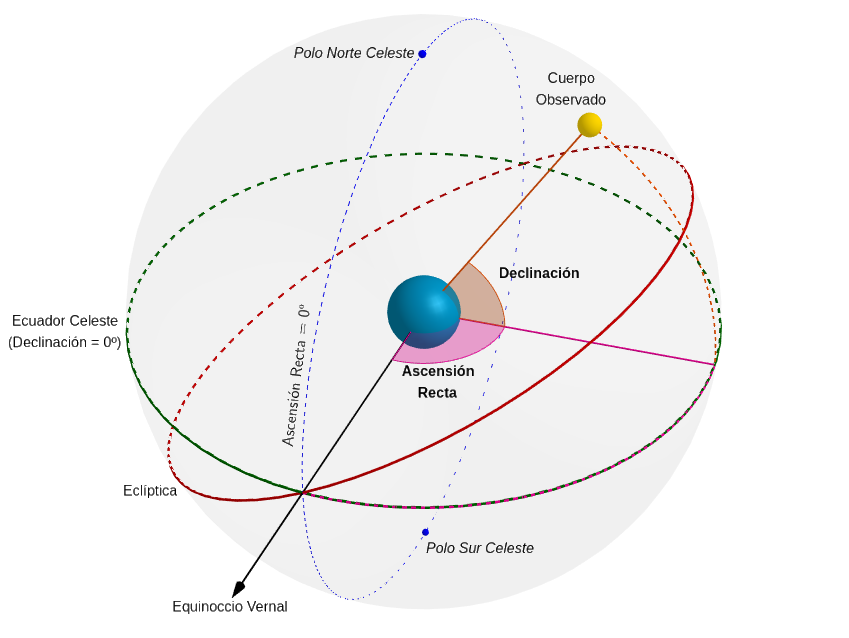
\includegraphics[scale=0.4]{images/ascension_declinacion.png}
\caption{La Tierra, en el centro, junto a la ascensión recta y declinación de cierto objeto. El círculo rojo define el camino aparente del Sol en el cielo, que define el plano de la eclíptica.}
\label{fig:ascension_declinacion}
\end{figure}

La declinación es medida en grados, como la latitud. Pero, a diferencia de la longitud, la ascensión recta es medida en horas, minutos y segundos en dirección este. Como en un día hay 24 horas, cada hora de ascensión recta corresponderá a una veinticuatroava parte de la rotación total de la Tierra, y por tanto, una hora será igual a $\frac{360}{24}=15º$.\\

Al conjunto de estas dos coordenadas junto a la distancia al objeto se les llama \textbf{Coordenadas Ecuatoriales}, y con ellas podremos definir la posición exacta de un objeto en cierto momento.\\

Dado que en ocasiones necesitaremos la posición del objeto en coordenadas cartesianas, veamos unas simples ecuaciones con las que pasaremos de coordenadas ecuatoriales a cartesianas \cite{moulton}.
\begin{align}
\left\{
\begin{array}{l}
	x = \rho \cos{\delta}\cos{\alpha}\\
	y = \rho \cos{\delta}\sin{\alpha}\\
	z = \rho \sin{\delta}
\end{array}
\right.
\label{eq:equatorial_to_cartesian}
\end{align}

Nótese que antes de aplicar estas ecuaciones deberemos pasar $\delta$ y $\alpha$ a radianes para utilizar las funciones trigonométricas. Las coordenadas $(x,y,z)$ tendrán la misma unidad que la distancia $\rho$.\\

\section{Caminos e ideas para desarrollar el método de determinación}
\label{sec:ideas_for_develope_method}
Una vez obtenidas las coordenadas ecuatoriales de un objeto mediante tres observaciones, las podemos escribir como un grupo de funciones de los elementos orbitales del cuerpo en el momento de las observaciones, $t_1, t_2, t_3$. Así, obtenemos lo siguiente:
\begin{align}
\left\{\begin{array}{l}
	\alpha_1 = \phi(a, e, \omega, i, \Omega, T; t_1)\\ 
	\alpha_2 = \phi(a, e, \omega, i, \Omega, T; t_2)\\ 
	\alpha_3 = \phi(a, e, \omega, i, \Omega, T; t_3)\\ 
	\delta_1 = \psi(a, e, \omega, i, \Omega, T; t_1)\\ 
	\delta_2 = \psi(a, e, \omega, i, \Omega, T; t_2)\\
	\delta_3 = \psi(a, e, \omega, i, \Omega, T; t_3)
\end{array}
\right.
\label{eq:ascension_declinacion}
\end{align}

Pues bien, el problema de determinación de órbitas consistirá en resolver todas estas ecuaciones para los seis elementos desconocidos, pero, las funciones de ascensión recta y declinación involucran a los elementos muy enrevesadamente, además de que son altamente trascendentales, es decir, no se pueden expresar en términos de funciones elementales.\\

La órbita a determinar podrá ser una elipse, una hipérbola o una parábola, y en los tres casos las coordenadas respecto a la Tierra se obtendrán mediante una serie de transformaciones trigonométricas, de manera que no dispondremos de soluciones directas para estas ecuaciones mediante métodos ordinarios.\\

El objetivo final del método de determinación es obtener la órbita del cuerpo observado, es decir, las coordenadas astronómicas que definen su movimiento. Pero, antes de todo, habremos de tratar el problema de encontrar cantidades intermedias con las que definir estas coordenadas, y como veremos más adelante (en \ref{subsec:orbital_elements}), a partir de la posición y la velocidad de un objeto en un instante $t$ se podrán obtener todos los elementos orbitales de éste.\\

Volvamos a las ecuaciones \eqref{eq:ascension_declinacion}, y supongamos que queremos encontrar las coordenadas polares y sus derivadas, por ejemplo, en $t=t_2$. Podemos reescribir las ecuaciones como:
\begin{align}
\left\{\begin{array}{l}
	\alpha_1 = f(\alpha_2, \delta_2, \rho_2, \alpha_2', \delta_2', \rho_2'; t_1, t_2)\\ 
	\alpha_2 = \alpha_2\\
	\alpha_3 = f(\alpha_2, \delta_2, \rho_2, \alpha_2', \delta_2', \rho_2'; t_2, t_3)\\
	\delta_1 = g(\alpha_2, \delta_2, \rho_2, \alpha_2', \delta_2', \rho_2'; t_1, t_2)\\
	\delta_2 = \delta_2\\
	\delta_3 = g(\alpha_2, \delta_2, \rho_2, \alpha_2', \delta_2', \rho_2'; t_2, t_3)
\end{array}
\right.
\label{eq:idea_laplace}
\end{align}

\noindent donde $\rho$ es la distancia al planeta en $t_2$ y:
\[
\alpha_2'=\frac{d\alpha}{dt}, \; \; \; \delta_2'=\frac{d\delta}{dt}, \; \; \; \rho_2'=\frac{d\rho}{dt} \; \; \;  \text{en} \; \; t=t_2
\]

Así, solo tendremos que resolver cuatro ecuaciones para cuatro incógnitas, pues $\alpha_2$ y $\delta_2$ son conocidas. Podremos modificar estas ecuaciones para hacer que sean más manejables a la hora de determinarlas, y, de hecho, este es el camino que toma \textbf{Laplace} a la hora de desarrollar su método, que fue aplicado por primera vez en 1780.\\

Por otra parte, podemos tomar tres coordenadas en dos momentos diferentes, $t_1$ y $t_3$, para así obtener otro conjunto de elementos a determinar, y haciéndonos así con dos ecuaciones con solamente dos incógnitas, que podrán ser resueltas.
\begin{align}
\left\{\begin{array}{l}
	\alpha_1 = \alpha_1\\
	\alpha_2 = F(\alpha_1, \delta_1, \rho_1, \alpha_3, \delta_3, \rho_3; t_1, t_2, t_3\\
	\alpha_3 = \alpha_3\\
	\delta_1 = \delta_1\\
	\delta_2 = G(\alpha_1, \delta_1, \rho_1, \alpha_3, \delta_3, \rho_3; t_1, t_2, t_3)\\
	\delta_3 = \delta_3
\end{array}
\right.
\label{eq:camino_gauss}
\end{align}

Este es el camino que siguió Lagrange para resolver el problema en 1778, y que retomó \textbf{Gauss} en 1801.\\

A pesar de la cantidad de estudios que se han realizado tras la publicación de estos métodos, muy poco de lo que es realmente nuevo o teóricamente importante se ha añadido a las determinaciones que desarrollaron Laplace y Gauss, a menos que se usen más de tres observaciones. \cite{moulton}\\


\section{Preparación y corrección de las observaciones}
Independientemente del método que queramos seguir para determinar la órbita del objeto observado, habremos de efectuar algunas correcciones en los datos obtenidos antes de comenzar a realizar cálculos, pues hay distintos factores que pueden hacer que la ascensión recta y declinación observadas difieran de su valor real.\\

En el equinoccio de primavera, que se corresponde con el punto Aries como comentamos anteriormente, la ascensión recta y declinación es nula, pues el plano de la eclíptica y el del ecuador de la Tierra se intersecan en dicho momento. Debido a la protuberancia de la Tierra en el ecuador, la Luna y el Sol causarán una ligera oscilación periódica y un lento cambio secular en la posición del plano de su ecuador. Así, los equinoccios no se corresponderán con un punto fijo y habrá pequeñas oscilaciones periódicas y lentos cambios de la posición de la Tierra a lo largo de la eclíptica, llamadas nutación y precesión. En este caso, se acostumbra a utilizar el equinoccio medio (equinoccio prescindiendo de la nutación) y la posición del ecuador al comienzo del año en el que se estén haciendo las observaciones para evitar el error en la ascensión recta y declinación.\\

Por otra parte, la observación del objeto cuya órbita queremos determinar también puede ser afectada por la aberración de la luz, es decir, la diferencia entre la posición observada del objeto y su posición real, causada por la combinación de la velocidad del observador (por la rotación de la Tierra) y la velocidad de la luz. Tendremos que corregir dos aberraciones: la anual, debida a la rotación de la Tierra alrededor del Sol, y la aberración diurna, debida a la rotación de la Tierra sobre su eje. Aún así, debido a que la velocidad de rotación sobre su eje es muy pequeña en comparación con la velocidad de traslación, la aberración diurna será relativamente pequeña, y podrá ser obviada, especialmente en el caso de que las observaciones tomadas no sea demasiado precisas. \cite{moulton}\\

Aunque no veamos la manera de hacer las correcciones sobre nuestras observaciones en este trabajo, es un paso a la hora de determinación muy importante y que deberá de ser gestionado en el momento que se quiera hacer una determinación de la órbita de un objeto mediante observaciones por telescopio.\\


\iffalse
\begin{comment}
Definamos como $\alpha_0$ y $\delta_0$ la ascensión recta y declinación del cuerpo observado en cierto momento, sin ninguna corrección previa. Entonces, sus valores referidos al equinoccio medio del comienzo del año, y corregidos para la aberración lumínica anual, son:
\[
\left\{
\begin{array}{l}
	\alpha = \alpha_0 - 15f - g \sin(G+\alpha_0) \tan(\delta_0) - h \sin(H+\alpha_0) \sec(\delta_0)\\
	\delta = \delta_0 - i \cos(\delta_0) - g \cos(G+\alpha_0) - h \cos(H+\alpha_0) \sin(\delta_0)
\end{array}
\right.
\]

\noindent donde $f, g, h, G$ y $H$ son cantidades auxiliares, a las que llamaremos \textit{números interestelares independientes}, y cuyo valor aparece en el \textit{American Ephemeris and Nautical Almanac} para cada día del año. Notar que estas correcciones serán expresadas en segundos de arco, pues en esta unidad son dadas las cantidades tomadas de la efemérides. Esta corrección será pequeña siempre que $\delta_0$ no sea cercano a $\pm90º$, pues cerca de dichos valores tanto la secante como la tangente que aparece en la corrección para $\alpha$ diverge.\\

Por último, tendremos que corregir la aberración diurna a través de las siguientes ecuaciones:
\[
\left\{
\begin{array}{l}
	\Delta \alpha = -0''.322 \cos(\phi) \cos(\theta - \alpha_0) \sec(\delta_0)\\
	\Delta \delta = -0''.322 \cos(\phi) \sin(\theta - \alpha_0) \sin(\delta_0)
\end{array}
\right.
\]

\noindent donde $\phi$ representará la latitud del observador y $\theta-\alpha_0$ representa el ángulo horario del objeto en el momento de la observación (\textit{???}). La primera corrección será pequeña mientras que $\delta_0$ no sea cercano a $\pm90º$, y la segunda no podrá exceder el valor de $0''.322$.\\

\textit{DUDAS: como se utilizan las dos correciones a la vez???? $0''.322$ se refiere a 0.322 segundos??}\\
\end{comment}
\fi


\section{Argumentación general para la determinación}
Los dos métodos más importantes para la determinación (Laplace y Gauss) siguen una estrategia similar, que expondremos a continuación. Para empezar, supongamos que solo disponemos de tres observaciones de nuestro objeto en tres momentos diferentes, $t_1, t_2, t_3$, de manera que conocemos la ascensión recta y declinación en cada uno de estos instantes. A continuación, definamos algunos términos:
\begin{itemize}
\item Definimos $C$, $S$ y $E$ como el cuerpo observado, el Sol (alrededor del cual gira $C$) y la Tierra respectivamente.
\item Sean $(\xi,\eta,\zeta)$ las coordenadas (cartesianas) de $C$ respecto a $E$, $(X,Y,Z)$ las coordenadas de $S$ respecto a $E$, y $(x,y,z)$ coordenadas de $C$ respecto a $S$.
\item $\rho$ es la distancia de $E$ a $C$, $r$ la distancia de $S$ a $C$ y $R$ la distancia de $E$ a $S$.
\end{itemize}

\begin{figure}[H]
\centering
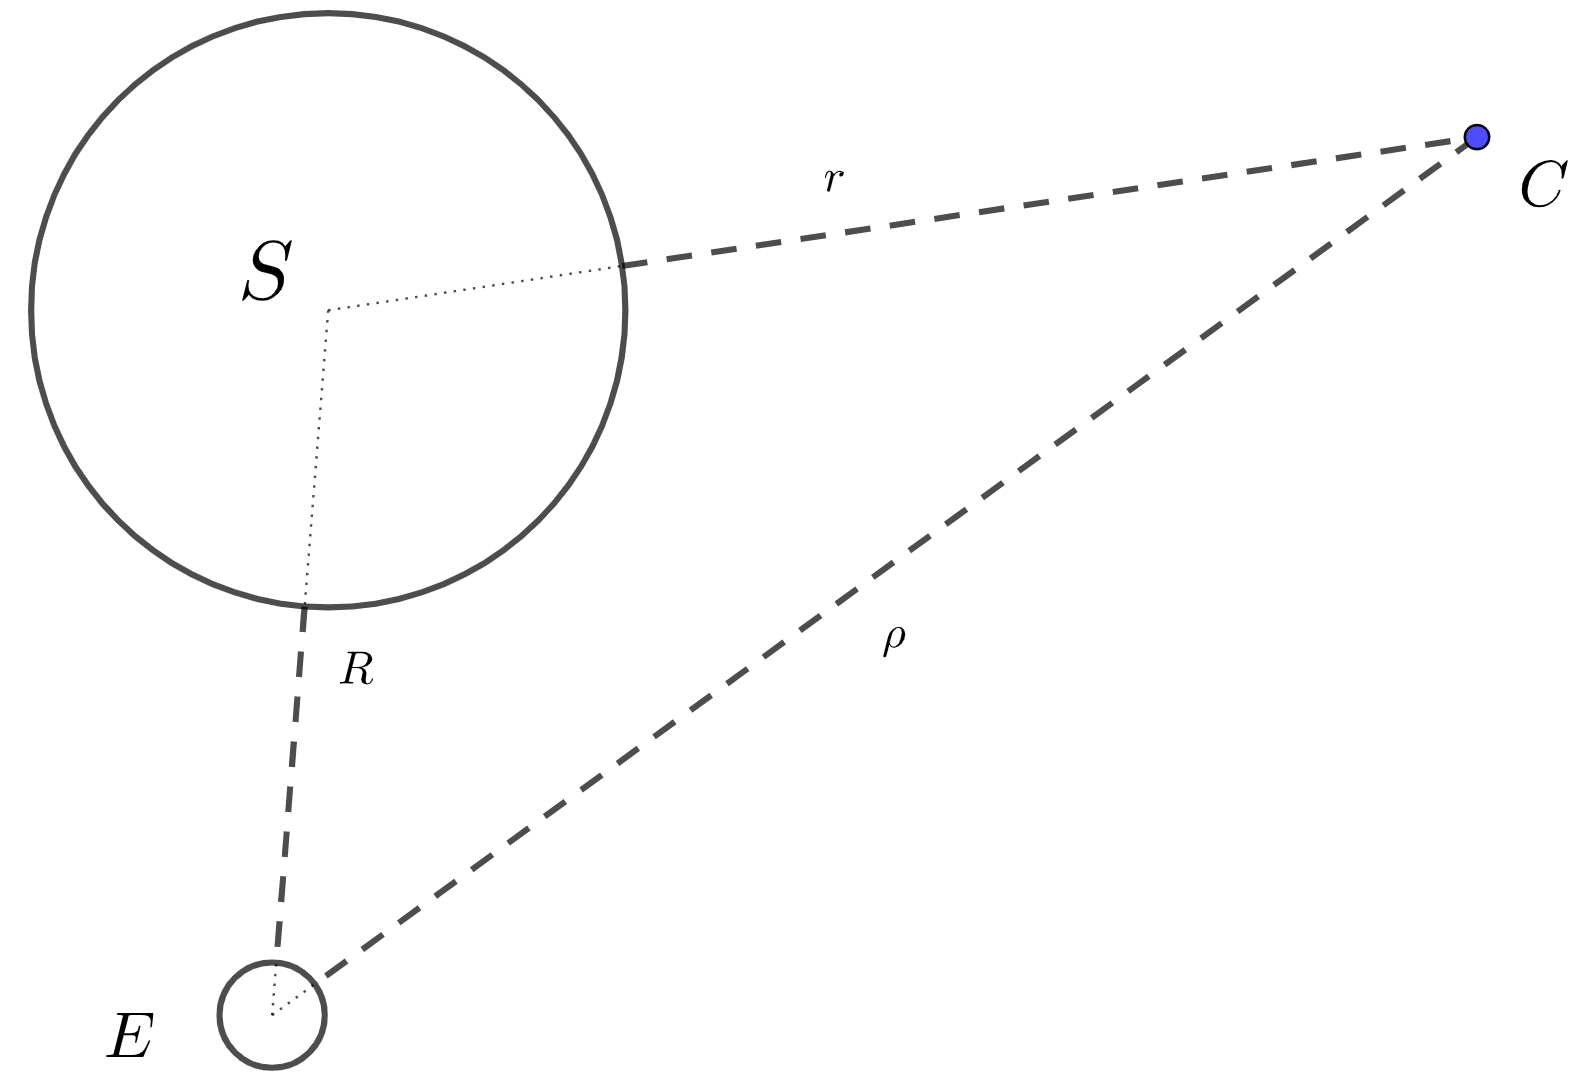
\includegraphics[scale=0.15]{images/notation.png}
\caption{Notación utilizada para nuestro problema}
\label{fig:notation}
\end{figure}

Con todo esto, podemos escribir:
\begin{align}
\left\{
\begin{array}{l}
\xi = \rho \cos{\delta}\cos{\alpha} = \rho\lambda\\
\eta = \rho \cos{\delta}\sin{\alpha} = \rho\mu\\
\zeta = \rho \sin{\delta} = \rho\nu
\end{array}
\right.
\label{eq:terminologia}
\end{align}
\noindent donde $(\lambda,\mu,\nu)$ es un vector unitario conocido que apunta de la Tierra al cuerpo observado, y el fin del estudio del problema será determinar $\rho$. \cite{moulton}\\

\section{Cambios en el plano de referencia.}
\label{sec:reference_plane}
Actualmente, la IAU (\textit{International Astronomical Union}) utiliza como sistema de coordenadas estándar el sistema ICRS (\textit{International Celestial Reference System}), del cuál deriva el plano ICRF (\textit{International Celestial Reference Frame}). De esta manera, a la hora de tomar la ascensión recta y declinación de un cuerpo lo obtendremos en el plano de referencia de la efemérides, es decir, en ICRF. El problema surge de que nuestro sistema de coordenadas tiene como base el plano de la eclíptica, que difiere de plano ICRF, y por tanto, tras obtener la posición y velocidad del cuerpo observado habremos de modificar las coordenadas para disponer de ellas en función del plano de la eclíptica \cite{ICRF}.\\

Para ser coherente con el ICRS y el origen de este (el baricentro del Sistema Solar), definimos el plano de la eclíptica como un plano que pasa por el origen del ICRS con una inclinación $\varepsilon_0$, que se corresponderá con la oblicuidad media, la inclinación del eje de la Tierra respecto al plano de la eclíptica \cite{ICRF} ($\approx23.4375º$ \cite{jpl}). Así, la transformación de las coordenadas del plano ICRF $(x,y,z)$ al plano de la eclíptica $(X,Y,Z)$ será:
\begin{align}
\left\{
\begin{array}{l}
	X=x\\
	Y=y\cos{\varepsilon_0}+z\sin{\varepsilon_0}\\
	Z=-y\sin{\varepsilon_0}+z\cos{\varepsilon_0}\\
\end{array}
\right.
\label{eq:ICRS_to_ecliptic}
\end{align}




\newpage
\thispagestyle{empty}



\chapter{Método Laplaciano de Determinación}
\label{chap:laplace_method}
En este capítulo se estudiará el método de Laplace para determinar la posición y velocidad de un objeto en un instante a utilizando tres observaciones (objetivo 2), y a partir de ellas determinaremos los elementos orbitales del cuerpo, pudiendo obtener así la elipse que describe en el espacio (objetivo 3).\\

Los pasos a seguir consistirán en aproximar las derivadas del vector unitario $(\lambda,\mu,\nu)$, así como las del vector $\overrightarrow{SE}$, determinar las distancias entre los tres cuerpos $S$, $E$, $C$, y con todo ello poder determinar la posición y velocidad del cuerpo respecto al Sol.\\

\section{Determinación de las derivadas de $\lambda$, $\mu$, $\nu$ en algún momento $t$.}
\label{sec:primera_segunda_derivada}
Dado que no podemos calcular el valor exacto de las derivadas de $\lambda$, $\mu$, $\nu$, utilizaremos fórmulas de derivación numérica con dos nodos para obtener un valor aproximado de éstas. Tomemos, por ejemplo, $t=t_2$, que por el momento nos bastará para demostrar que se puede realizar una buena aproximación. Supongamos que el valor de $\lambda'$ no cambia muy rápido; entonces, el valor de la derivada en $t_2$ en el intervalo $[t_1,t_2]$ será muy cercano al valor de:
\[
\lambda_{12}'=\frac{\lambda(t_2)-\lambda(t_1)}{t_2-t_1},
\]

\noindent y ya que los nodos elegidos cumplen $t_2>t_1$, estaremos ante una diferencia regresiva. Análogamente podremos aproximar el valor de la derivada en $t_2$ mediante una diferencia progresiva, a la que llamaremos $\lambda_{23}'$.\\

El error de estas aproximaciones, suponiendo que $\lambda$ sea de clase 2 en el intervalo de aproximación, es del orden de $(t_2-t_1)$ y $(t_3-t_2)$ para $\lambda_{12}'$ y $\lambda_{23}'$ respectivamente. Por tanto, cuanto más pequeño sea el intervalo donde realizamos las operaciones, es de esperar que la aproximación obtenida sea mejor. Además, si la longitud del intervalo $[t_1,t_2]$ es igual a la longitud de $[t_2,t_3]$, podremos calcular el valor aproximado de $\lambda'$ en $t_2$ mediante una diferencia centrada, obteniendo:
\[
\lambda'_2=\frac{\lambda_{12}'+\lambda_{23}'}{2}
\]

Si los intervalos tienen una longitud diferente, podremos ajustar la disparidad entre ellos para realizar la aproximación o utilizar un método diferente para aproximar la derivada, como veremos en \ref{sec:series_potencias}.\\

Análogamente podremos definir la derivada segunda de $\lambda$ en $t_2$, en la que utilizaremos los valores de la primera derivada obtenidos anteriormente:
\[
\lambda''_2=\frac{\lambda_{23}'-\lambda_{12}'}{\frac{1}{2}(t_3-t_1)}
\]

Dicha aproximación será de orden $(t_3-t_1)^2$ siempre que $\lambda\in\mathcal{C}^4[t_1,t_3]$. Mediante este mismo método calcularemos la primera y segunda derivada de $\mu$ y $\nu$; además, podemos suponer que las tres funciones son de clase infinito en todo $\mathbb{R}$.\\

Como hemos comentado antes, las aproximaciones obtenidas de esta manera es razonable que sean más cercanas cuanto menor sea la longitud de los intervalos entre las observaciones, y generalmente, en la práctica, los intervalos que utilizaremos serán cortos.\\

Finalmente, necesitaremos tener los valores de la primera y segunda derivada de $X$, $Y$, $Z$, correspondientes al vector de $S$ a $E$, aunque no tendremos por qué calcularlos de manera aproximada. Para obtener dichas cantidades exactas utilizaremos la efemérides proporcionada por el \href{https://ssd.jpl.nasa.gov/horizons.cgi}{\textit{Jet Propulsion Laboratory}} en su página web, que nos dará el valor de estas variables para cualquier día del año, a cualquier hora y desde cualquier coordenada terrestre. Notar que aquí solo aparecerá la posición y velocidad, pero dado que $E$ gira alrededor de $S$ en concordancia con la ley de Gravitación Universal, podremos calcular la segunda derivada mediante:
\begin{align}
\left\{
\def\arraystretch{2}
\begin{array}{l}
	X'' = -\ddfrac{k^2X}{R^3}\\
	Y'' = -\ddfrac{k^2Y}{R^3}\\
	Z'' = -\ddfrac{k^2Z}{R^3}
\end{array}
\right.
\label{eq:ley_gravitacion_S_E}
\end{align}

\noindent donde $k^2=GM$\footnote{Es más común ver este valor como $\mu$, pero para evitar confusiones con la segunda coordenada del vector unitario $\overrightarrow{EC}$ utilizaremos el nombre de $k^2$.}, parámetro gravitacional estándar, $G=6.674\times10^{-11}\frac{\text{N}\cdot\text{m}^2}{\text{kg}^2}$ constante de gravitación y $M=1.989\times10^{30}\;\text{kg}$ masa del Sol. Tomamos solo la masa del Sol, $M$, ya que la masa de nuestro cuerpo es despreciable en comparación con ésta usando como modelo el problema de Kepler.\\


\markedsection{$C$ gira en torno a $S$ de acuerdo a la ley de gravitación.}{Imponer la condición de que $C$ gira en torno a $S$ de acuerdo a la ley de gravitación.}
\label{sec:ley_gravitacion}
Asumiendo que el cuerpo observado $C$ no está alterado por la interacción con otros cuerpos cercanos, podemos asegurar que cumplirá el problema de Kepler, dando lugar a las siguientes ecuaciones diferenciales:
\begin{align}
\left\{
\def\arraystretch{2}
\begin{array}{l}
	\ddfrac{d^2x}{dt^2}=-\ddfrac{k^2x}{r^3}\\
	\ddfrac{d^2y}{dt^2}=-\ddfrac{k^2y}{r^3}\\
	\ddfrac{d^2z}{dt^2}=-\ddfrac{k^2z}{r^3}
\end{array}
\right.
\label{eq:ley_gravitacion_S_C}
\end{align}

\noindent análogas a las que hemos visto para $S$ y $E$ en \eqref{eq:ley_gravitacion_S_E}.\\

Además, utilizando las \hyperref[eq:terminologia]{relaciones entre $E$, $C$ y $S$}, así como los resultados vistos anteriormente, llegamos a:
\begin{align}
\left\{
\begin{array}{l}
	x=\rho\lambda-X\\
	y=\rho\mu-Y\\
	z=\rho\nu-Z
\end{array}
\right.
\label{eq:relacion_C_S_E}
\end{align}

\noindent y sustituyendo los valores obtenidos en las  ecuaciones \eqref{eq:ley_gravitacion_S_C}, obtenemos:
\begin{align}
\left\{
\def\arraystretch{2}
\begin{array}{l}
	(\rho\lambda)'' - X'' = \ddfrac{-k^2(\rho\lambda-X)}{r^3}\\
	(\rho\mu)'' - Y'' = \ddfrac{-k^2(\rho\mu-Y)}{r^3}\\
	(\rho\nu)'' - Z'' = \ddfrac{-k^2(\rho\nu-Z)}{r^3}
\end{array}
\right.
\label{eq:derivada_segunda}
\end{align}

Desarrollando la segunda derivada de $\rho\lambda$ llegamos a:
\[
(\rho\lambda)''=(\rho'\lambda+\rho\lambda')'=\rho''\lambda+2\rho'\lambda'+\rho\lambda'',
\]

\noindent valor que utilizaremos más adelante.\\

Utilizando el resultado \eqref{eq:ley_gravitacion_S_E}, sustituyendo en la ecuación \eqref{eq:derivada_segunda} y desarrollando llegamos a lo siguiente:
\begin{align}
\left\{
\def\arraystretch{2}
\begin{array}{l}
	\lambda\rho''+2\lambda'\rho'+[\lambda''+\ddfrac{k^2\lambda}{r^3}]\rho=-k^2X[\ddfrac{1}{R^3}-\ddfrac{1}{r^3}]\\
	\mu\rho''+2\mu'\rho'+[\mu''+\ddfrac{k^2\mu}{r^3}]\rho=-k^2Y[\ddfrac{1}{R^3}-\ddfrac{1}{r^3}]\\
	\nu\rho''+2\nu'\rho'+[\nu''+\ddfrac{k^2\nu}{r^3}]\rho=-k^2Z[\ddfrac{1}{R^3}-\ddfrac{1}{r^3}]
\end{array}
\right.
\label{eq:fundamental_equations}
\end{align}

\noindent a las que llamaremos ecuaciones fundamentales. Así, las incógnitas de las ecuaciones a resolver pasan a ser $r, \; \rho, \; \rho'$ y $\rho''$.\\



\section{Determinación de las distancias de $C$ a $E$ y $S$.}
\label{sec:distancias}
Actualmente disponemos de un vector unitario $(\lambda,\mu,\nu)$ que apunta desde la Tierra hacia el cuerpo observado, pero desconocemos la distancia que hay entre estos dos cuerpos. Para determinar tanto esta distancia como la que hay desde $S$ hasta $C$, utilizaremos las ecuaciones fundamentales obtenidas al final del paso anterior, \eqref{eq:fundamental_equations}, y una condición geométrica que cumplirán los tres cuerpos. Para llevar a cabo esto, tomaremos el sistema \eqref{eq:fundamental_equations} como un sistema lineal en $\rho$, $\rho'$ y $\rho''$ y resolveremos utilizando la regla de Cramer. Comencemos definiendo el siguiente determinante:
\[
D =
\left|
\begin{array}{ccc}
	\lambda & 2\lambda' & \lambda''+\frac{k^2\lambda}{r^3}\\
	\mu & 2\mu' & \mu''+\frac{k^2\mu}{r^3}\\
	\nu & 2\nu' & \nu''+\frac{k^2\nu}{r^3}
\end{array}
\right|
=
2
\left|
\begin{array}{ccc}
	\lambda & \lambda' & \lambda''\\
	\mu & \mu' & \mu''\\
	\nu & \nu' & \nu''
\end{array}
\right|
=2W(\lambda,\mu,\nu)
\]

\noindent siendo $W(\lambda,\mu,\nu)$ el Wronskiano de las coordenadas angulares. La segunda forma del determinante ha sido obtenida mediante la transformación $C_3-\frac{k^2\lambda}{r^3}C_1$ sobre la matriz, donde $C_i$ representará la columna i-ésima. Una vez hayamos sustituido las derivadas exactas por su valor aproximado calculado anteriormente, conoceremos todas las cantidades de este determinante.\\

Por otra parte, definiremos el determinante $D_1$, que utilizaremos para calcular $\rho$ mediante la regla de Cramer, reemplazando la tercera columna por los términos independientes del sistema \eqref{eq:fundamental_equations} y omitiendo el factor $[\frac{1}{R^3}-\frac{1}{r^3}]$, que añadiremos más adelante. De nuevo, conocemos todas las cantidades utilizadas. Así, obtenemos el siguiente determinante:
\[
D_1 = -2k^2
\left|
\begin{array}{ccc}
\lambda & \lambda' & X\\
\mu & \mu' & Y\\
\nu & \nu' & Z
\end{array}
\right|
\]

Con todo esto, la distancia $\rho$ será determinada por:
\[
\rho = \frac{D_1}{D}[\frac{1}{R^3}-\frac{1}{r^3}],
\]

El valor de $r$ es desconocido, por lo que añadiremos la siguiente ecuación formando con la anterior un sistema de ecuaciones en $r$ y $\rho$.
\begin{align}
r^2=\rho^2+R^2-2\rho R\cos\psi,
\label{eq:triangle_relations_1}
\end{align}

\noindent donde $\psi$ es el ángulo formado en $E$ trazando una línea imaginaria hasta el Sol y hasta el cuerpo observado, es decir, entre $R$ y $\rho$; esta ecuación expresa el hecho de que $S$, $E$ y $C$ forman un triángulo como vimos en la \hyperref[figure:1]{figura 1}.\\

Dado que disponemos de los valores $\overrightarrow{SE}=(X,Y,Z)$ y $\overrightarrow{EC}=(\lambda,\mu,\nu)$, vector unitario, podremos obtener el coseno de $\psi$ con:
\[
\cos{\psi}=\frac{\langle\overrightarrow{SE},\overrightarrow{EC}\rangle}{|\overrightarrow{SE}||\overrightarrow{EC}|}=\frac{\langle(X,Y,Z),(\lambda,\mu,\nu)\rangle}{R}
\]

Resolviendo el sistema de ecuaciones al que hemos llegado obtendremos los valores de $\rho$ y $r$, habiendo terminado este paso. Más adelante discutiremos la unicidad de la solución en el sistema con $r,\rho>0$ (\ref{chap:soluciones_admisibles}). Al encontrar la solución de este sistema podremos calcular las coordenadas de $C$ mediante las ecuaciones \eqref{eq:relacion_C_S_E} de las relaciones entre $S$, $E$ y $C$.\\

\section{Determinación de las componentes de velocidad de $C$.}
\label{sec:velocity_component}
Se sigue de las ecuaciones \eqref{eq:relacion_C_S_E} que:
\begin{align}
\left\{
\begin{array}{l}
	x'=\rho'\lambda+\rho\lambda'-X'\\
	y'=\rho'\mu+\rho\mu'-Y'\\
	z'=\rho'\nu+\rho\nu'-Z'
\end{array}
\right.
\label{eq:relacion_C_S_E_derivada}
\end{align}

En estas ecuaciones solo tenemos una incógnita, $\rho'$, que podremos determinar resolviendo por Cramer en \eqref{eq:fundamental_equations} a partir de:
\[
\rho'=+\frac{D_2}{D}[\frac{1}{R^3}-\frac{1}{r^3}],
\; \; \; \; \; \; \; \; \; \text{ con } \;
D_2 = -k^2
\left|
\begin{array}{ccc}
\lambda & X & \lambda''\\
\mu & Y & \mu''\\
\nu & Z & \nu''
\end{array}
\right|
\]

Notar que en $D_2$ también hemos realizado la operación $C_3-\frac{k^2\lambda}{r^3}C_1$, como en $D$, para obtener un determinante más simple.\\

Dado que ya conocemos el valor de $r$ podremos calcular directamente $\rho'$, y de esta manera $x'$, $y'$ y $z'$ se vuelven conocidas.\\

\markedsection{Determinación de los elementos orbitales.}{Determinación de los elementos orbitales a partir de la posición y velocidad del cuerpo observado.}
\label{sec:elements_determination}
Una vez conocida tanto la posición como la velocidad del cuerpo en un instante determinado, nos dispondremos a calcular los elementos orbitales mediante las distintas fórmulas estudiadas en el manual de Mecánica Celeste\cite{ortega}. Denotemos por $r(t)=(x,y,z)(t)$ la posición del objeto y $v(t)$ su derivada, la velocidad.\\

Comencemos determinando la energía que tiene nuestro cuerpo en un instante $t$. Para ello utilizaremos:
\[
h=\frac{|v(t)|^2}{2}-\frac{\mu}{|r(t)|}
\]

\noindent donde $\mu=GM$ una constante positiva. Con el valor de la energía podemos pasar a calcular la primera de nuestros elementos astronómicos, la longitud del semieje mayor, $a$, utilizando la siguiente ecuación:
\[
a=-\frac{\mu}{2h}
\]

Pasemos ahora a calcular el momento angular de nuestro objeto. Dado que la masa del objeto observado es despreciable frente a la masa del Sol, podremos obviar su valor, obteniendo así el vector del momento angular mediante:
\[
c=r(t)\wedge v(t)
\]

Calculado el momento angular, podremos obtener el vector de excentricidad para la órbita del cuerpo observado:
\[
\vec{e}=-\frac{r(t)}{|r(t)|}-\frac{1}{\mu}(c\wedge v(t))
\]

\noindent y la excentricidad de la órbita será $e=|\vec{e}|$.\\

Una vez obtenidos estos valores, podemos utilizaremos la tercera ley de Kepler para obtener el período mínimo (suponiendo que nuestra órbita se corresponda con la de una elipse). Si el momento angular del objeto observado $c\neq0$ y su energía $h<0$, entonces la órbita es periódica y su período mínimo valdrá:
\[
p=\frac{2\pi}{\sqrt{\mu}}a^{3/2}
\]

Sabemos que el vector del momento angular, del que disponemos, es el vector normal al plano orientado de la órbita, pudiendo calcular así la inclinación del plano de movimiento. Además, calculando la intersección de éste con el plano de la eclíptica obtenemos la línea de nodos y con ella el nodo ascendente $\mathcal{N}_+$, con la que podremos determinar $\Omega$.
\[
\left\{
\begin{array}{l}
	i=\measuredangle(\vec{e}_3,\vec{n}), \; \; \; \; \; \; \; \; \; \; i\in]0,\pi[\\
	\Omega=\measuredangle(\vec{e}_1, \mathcal{N}_+), \; \; \; \; \; \Omega\in\mathbb{R}/2\pi\mathbb{Z}
\end{array}
\right.
\]

Finalmente usaremos el vector de excentricidad $\vec{e}$ para calcular $\omega$, utilizando el nodo ascendente como eje de rotación.\\


\markedsection{Derivadas de $\lambda$, $\mu$, $\nu$ mediante interpolación.}{Determinación de las derivadas de $\lambda$, $\mu$, $\nu$ mediante interpolación.}
\label{sec:series_potencias}
Tal y como hemos visto en la sección \ref{sec:primera_segunda_derivada}, hemos de calcular la primera y segunda derivada de las coordenadas angulares $\lambda$, $\mu$, $\nu$. El problema es que no siempre los intervalos de tiempo en los que hacemos la medida del objeto en el cielo son equiespaciados, y por tanto no podremos obtener una aproximación mediante diferencias centradas. Por tanto, busquemos un nuevo método para obtener las derivadas aproximadas de nuestras coordenadas angulares.\\

Comencemos recordando las ecuaciones \eqref{eq:ley_gravitacion_S_C}:
\begin{align}
\left\{
\def\arraystretch{2}
\begin{array}{l}
	\ddfrac{d^2x}{dt^2}=-\ddfrac{k^2x}{r^3}\\
	\ddfrac{d^2y}{dt^2}=-\ddfrac{k^2y}{r^3}\\
	\ddfrac{d^2z}{dt^2}=-\ddfrac{k^2z}{r^3}
\end{array}
\right.
\label{eq:ley_gravitacion_C_2}
\end{align}

La solución para estas ecuaciones diferenciales de segundo orden puede ser expandida como serie de Taylor en $t$, y esta convergerá siempre que el valor de $t$ no sea especialmente grande.
\begin{align}
\left\{
\def\arraystretch{2}
\begin{array}{l}
	x=x_0+x_0't+\ddfrac{1}{2}(\ddfrac{d^2x}{dt^2})_0t^2+...+\ddfrac{1}{n!}(\ddfrac{d^nx}{dt^n})_0t^n+...\\
	y=y_0+y_0't+\ddfrac{1}{2}(\ddfrac{d^2y}{dt^2})_0t^2+...+\ddfrac{1}{n!}(\ddfrac{d^ny}{dt^n})_0t^n+...\\
	z=z_0+z_0't+\ddfrac{1}{2}(\ddfrac{d^2z}{dt^2})_0t^2+...+\ddfrac{1}{n!}(\ddfrac{d^nz}{dt^n})_0t^n+...\\	
\end{array}
\right.
\label{eq:series_taylor}
\end{align}

En las ecuaciones superiores el subíndice 0 indicará que tomamos el valor $t=0$ en la función. Podemos sustituir la segunda derivada que aparece en estas series por su valor en \eqref{eq:ley_gravitacion_C_2}, la tercera derivada por la derivada de ésta y a partir de la cuarta derivada repetimos este proceso, teniendo así que las series estarán solo en función de la $x$, $y$, $z$ y la primera derivada de cada una de estas, todos ellas tomadas en $t=0$.\\

Los tres valores $x$, $y$, $z$, a los que en conjunto llamaremos $r(t)$, forman una solución del problema de Kepler. Además, sabemos que la fórmula de las soluciones para el problema de Kepler es:
\[
r(t)=a(\cos{u(t)}-e,\sqrt{1-e^2}\sin{u(t)})
\]

\noindent donde $u(t)$ es la anomalía. Dado que la ecuación está formada por funciones trigonométricas, que son analíticas, y la anomalía es una función analítica por el teorema de la función implícita, llegamos a que $r(t)$ será también una función analítica.\\

Hemos de tener en cuenta que el valor de estas series no siempre tiene valor práctico, pues el intervalo de tiempo para la convergencia puede ser demasiado grande; notar que los límites serán más pequeños cuanto más pequeña sea la distancia del perihelio y más grande la excentricidad de nuestra órbita.\\

En el caso de la Tierra, expandiendo sus coordenadas en series de potencias, obtendremos una convergencia durante largos intervalos de tiempo debido a la pequeña excentricidad de la órbita terrestre ($e\approx0.0167$). Así, se sigue de la ecuación \eqref{eq:relacion_C_S_E}, que relaciona las coordenadas de la Tierra, el Sol y el cuerpo observado que las ecuaciones de $\rho$, $\lambda$, $\mu$, $\nu$ también son funciones analíticas y por ello podrán ser expandidas como series de Taylor, con el mismo rango de utilidad que el de las series para $x$, $y$ y $z$.\\

Veamos las series para $\lambda$, pues las de $\mu$ y $\nu$ serán simétricamente similares. Tomando los valores $t_1$, $t_2$ y $t_3$, las series para $\lambda$ serán:
\begin{align}
\left\{
\begin{array}{l}
	\lambda(t)=c_0+c_1t+c_2t^2+...\\
	\lambda(t_1)=c_0+c_1t_1+c_2t_1^2+...\\
	\lambda(t_2)=c_0+c_1t_2+c_2t_2^2+...\\
	\lambda(t_3)=c_0+c_1t_3+c_2t_3^2+...
\end{array}
\right.
\label{eq:series_lambda}
\end{align}

\noindent donde los valores $c_0, c_1, c_2, ...$ son constantes. Si estas series terminan tras los términos elevados al cuadrado, podremos determinar $c_0$, $c_1$ y $c_2$ resolviendo como un sistema de ecuaciones, ya que conocemos las cantidades $\lambda(t_1)$, $\lambda(t_2)$, $\lambda(t_3)$. Así, tenemos que cuantas más observaciones tengamos disponibles, más coeficientes podrán ser determinados.\\

Tomamos ahora el sistema de ecuaciones \eqref{eq:series_lambda}; si queremos que sea compatible, su determinante ha de ser 0, pues tenemos tres incógnitas y cuatro ecuaciones, es decir, nos ``sobra'' una ecuación (sistema compatible indeterminado). Así, podemos obtener la siguiente igualdad:
\begin{align}
\left|
\begin{array}{cccc}
\lambda(t)   & 1 & t   & t^2  \\
\lambda(t_1) & 1 & t_1 & t^2_1\\
\lambda(t_2) & 1 & t_2 & t^2_2\\
\lambda(t_3) & 1 & t_3 & t^2_3\\
\end{array}
\right|
=0
\label{eq:resultante}
\end{align}

Si resolvemos este determinante desarrollando por la primera columna y despejamos $\lambda$ obtenemos:
\begin{align}
\lambda(t)_L=
\frac{(t-t_2)(t-t_3)}{(t_1-t_2)(t_1-t_3)}\lambda(t_1)
+\frac{(t-t_3)(t-t_1)}{(t_2-t_3)(t_2-t_1)}\lambda(t_2)
+\frac{(t-t_1)(t-t_2)}{(t_3-t_1)(t_3-t_2)}\lambda(t_3)
\label{eq:lambda_value}
\end{align}

Utilizamos el subíndice $L$ para denotar que esta función es aproximada y no proporcionará el valor exacto de $\lambda$ (salvo en ciertos casos).\\

Dicho polinomio corresponderá al polinomio de interpolación de Lagrange con el que obtendremos un valor aproximado de $\lambda$. Hemos de tener en cuenta que los valores en los nodos $t_1$, $t_2$, $t_3$ han de ser diferentes entre sí para que no se anulen los denominadores.\\

Con esto, somos capaces de obtener $\lambda$ de manera exacta en $t_1$, $t_2$ y $t_3$; para otros valores diferentes de $t$ obtendremos $\lambda$ de forma aproximada. Para obtener un valor exacto de $\lambda$ habremos de tomar la primera ecuación de \eqref{eq:series_lambda}, una serie infinita, dentro de su rango de convergencia.\\

Como comentamos anteriormente, el polinomio de interpolación de Lagrange obtenido nos proporcionará valores aproximados de $\lambda$, por lo que será conveniente estudiar el error de éste, que tomando la primera ecuación de \eqref{eq:series_lambda} será:
\[
|\lambda(t)-\lambda_L(t)|
\]

Dado que en anteriores secciones hemos supuesto que $\lambda$, $\mu$, $\nu$ son de clase infinito, podemos aplicar el teorema de error de interpolación, que nos dará una fórmula para obtener el error para todo $t$. Utilizando los tres nodos $t_1$, $t_2$, $t_3$ obtenemos:
\begin{align}
|\lambda(t)-\lambda_L(t)|=\ddfrac{\lambda^{\romannumeral 4}(\xi)}{4!}|t-t_1||t-t_2||t-t_3|
\label{eq:interpolation_error}
\end{align}

\noindent donde $\min{(t,t_1,t_2,t_3)}<\xi<\max{(t,t_1,t_2,t_3)}$. El cálculo de $\xi$ es complicado, pero podremos tomar una cota superior para $\lambda^{\romannumeral 4}$. Sea $K_4$ dicha cota, con $|\lambda^{\romannumeral 4}(x)|\leq K_4$, entonces el error de la interpolación será:
\begin{align}
|\lambda(t)-\lambda_L(t)|\leq\ddfrac{K_4}{4!}|t-t_1||t-t_2||t-t_3|
\label{eq:interpolation_error_cota}
\end{align}

Utilizando un mayor número de observaciones dispondremos de más nodos; así, si hemos realizado $N$ observaciones, la ecuación para el error será:
\begin{align}
|\lambda(t)-\lambda_L(t)|\leq\ddfrac{K_N}{(N+1)!}|t-t_1|...|t-t_N|
\label{eq:interpolation_error_n_observations}
\end{align}

Con el estudio del error y todo lo visto anteriormente, podemos justificar que la diferencia entre los valores de $t$ ha de ser pequeña en la práctica para que las cantidades aproximadas calculadas sean lo más cercanas a su valor original. Además, no tendría sentido una diferencia de tiempo muy grande entre las observaciones del objeto, pues pasaríamos mucho tiempo para determinar una única órbita.\\

Por último, ya que necesitamos la primera y segunda derivada de $\lambda$, nos bastará con derivar del polinomio \eqref{eq:lambda_value}.
\begin{align*}
\lambda'(t)_L = \frac{2t-(t_2+t_3)}{(t_1-t_2)(t_1-t_3)}\lambda(t_1)
+\frac{2t-(t_3+t_1)}{(t_2-t_3)(t_2-t_1)}\lambda(t_2)
+\frac{2t-(t_1+t_2)}{(t_3-t_1)(t_3-t_2)}\lambda(t_3)\\
\lambda''(t)_L = \frac{2}{(t_1-t_2)(t_1-t_3)}\lambda(t_1)
+\frac{2}{(t_2-t_3)(t_2-t_1)}\lambda(t_2)
+\frac{2}{(t_3-t_1)(t_3-t_2)}\lambda(t_3)
\end{align*}

Tal y como comentamos anteriormente, se procederá al cálculo de $\mu$ y $\nu$ y al estudio de su error de aproximación de manera similar a la desarrollada en este apartado.\\

\newpage
\thispagestyle{empty}



\chapter{Número de soluciones admisibles}
\label{chap:soluciones_admisibles}
Tal y como comentamos en \ref{sec:distancias}, al obtener el valor de $\rho$ y $r$ puede que obtengamos más de una solución posible, por lo que es conveniente estudiar cuál de estas soluciones es válida para nuestro problema y cuál no, y dentro de las válidas determinar cuál es la solución que nos lleva a la órbita real del cuerpo observado (objetivo 4).\\

También trataremos de acotar el intervalo de valores donde la solución del problema de determinación es única.\\

\section{Ecuaciones fundamentales en el método de Laplace.}
\label{sec:fundamental_equations}
Una vez terminada la explicación del método de determinación con tres observaciones, recapitulemos viendo las principales ecuaciones utilizadas para obtener las distancias del objeto observado. Las ecuaciones fundamentales serán las de \eqref{eq:fundamental_equations}, que involucrarán las coordenadas angulares $\lambda$, $\mu$, $\nu$ y sus derivadas, las cuáles conocemos su valor aproximado por \ref{sec:primera_segunda_derivada} o \ref{sec:series_potencias}. Por otra parte, el valor de $\rho$ y sus derivadas se obtendrá resolviendo las ecuaciones fundamentales utilizando la regla de Cramer, como vimos en anteriores apartados, aunque discutiremos más adelante otro método para su cálculo.\\

Hasta ahora disponemos de $\rho$ y $\rho'$; nos faltaría por calcular $\rho''$. Comencemos definiendo el determinante $D_3$:
\[
D_3=-2k^2
\left|
\begin{array}{ccc}
X & \lambda' & \lambda''\\
Y & \mu' & \mu''\\
Z & \nu' & \nu''
\end{array}
\right|
\]

Tras ello, calculemos el determinante $D$ cambiando la primera columna por el término independiente de \eqref{eq:fundamental_equations}, sin tomar $[\frac{1}{R^3}-\frac{1}{r^3}]$. 
\[
\left|
\begin{array}{ccc}
-k^2X & 2\lambda' & \lambda''+\frac{k^2\lambda}{r^3}\\
-k^2Y & 2\mu' & \mu''+\frac{k^2\mu}{r^3}\\
-k^2Z & 2\nu' & \nu''+\frac{k^2\nu}{r^3}
\end{array}
\right|
=-2k^2
\left|
\begin{array}{ccc}
X & \lambda' & \lambda''\\
Y & \mu' & \mu''\\
Z & \nu' & \nu''
\end{array}
\right|
-\frac{2k^4}{r^3}
\left|
\begin{array}{ccc}
X & \lambda' & \lambda\\
Y & \mu' & \mu\\
Z & \nu' & \nu
\end{array}
\right|
=
D_3-\frac{k^2D_1}{r^3}
\]

El signo negativo delante del determinante $D_1$ aparece por intercambiar la primera y la tercera columna del determinante inmediatamente anterior.\\

Así, tenemos que los valores de $\rho$ y sus derivadas pueden ser calculados mediante:
\begin{align}
\left\{
\def\arraystretch{1.5}
\begin{array}{l}
	\rho   = \ddfrac{D_1}{D}[\ddfrac{1}{R^3}-\ddfrac{1}{r^3}]\\
	\rho'  = \ddfrac{D_2}{D}[\ddfrac{1}{R^3}-\ddfrac{1}{r^3}]\\
	\rho'' = \ddfrac{1}{D}[D_3-\ddfrac{k^2D_1}{r^3}][\ddfrac{1}{R^3}-\ddfrac{1}{r^3}]
\end{array}
\right.
\label{eq:rho_values}
\end{align}

\noindent con $D$, $D_1$ y $D_2$ definidos anteriormente.\\

Notar que los determinantes $D$, $D_1$, $D_2$, $D_3$ están sujetos a pequeños errores dado que los valores implicados en ellos no pueden ser calculados de forma exacta, procediendo a obtenerlos de manera aproximada. Además, trabajamos bajo el supuesto de que las observaciones al objeto son realizadas desde el centro de la Tierra, y no desde un punto concreto de ella. Tras haber calculado de forma aproximada las distancias podremos corregir dichas observaciones por los efectos de la posición del observador sobre un punto en la superficie de la Tierra. \cite{moulton}\\






\section{Ecuaciones para la determinación de las distancias $r$ y $\rho$.}
\label{sec:distancias_r_rho}
Recordemos la imagen \ref{fig:notation} en la que mostrábamos el triángulo formado por los tres cuerpos $S$, $E$ y $C$ junto a sus distancias. Definamos $\psi$ y $\phi$, ángulos formados en $E$ y $C$ respectivamente.

\begin{figure}[H]
\centering
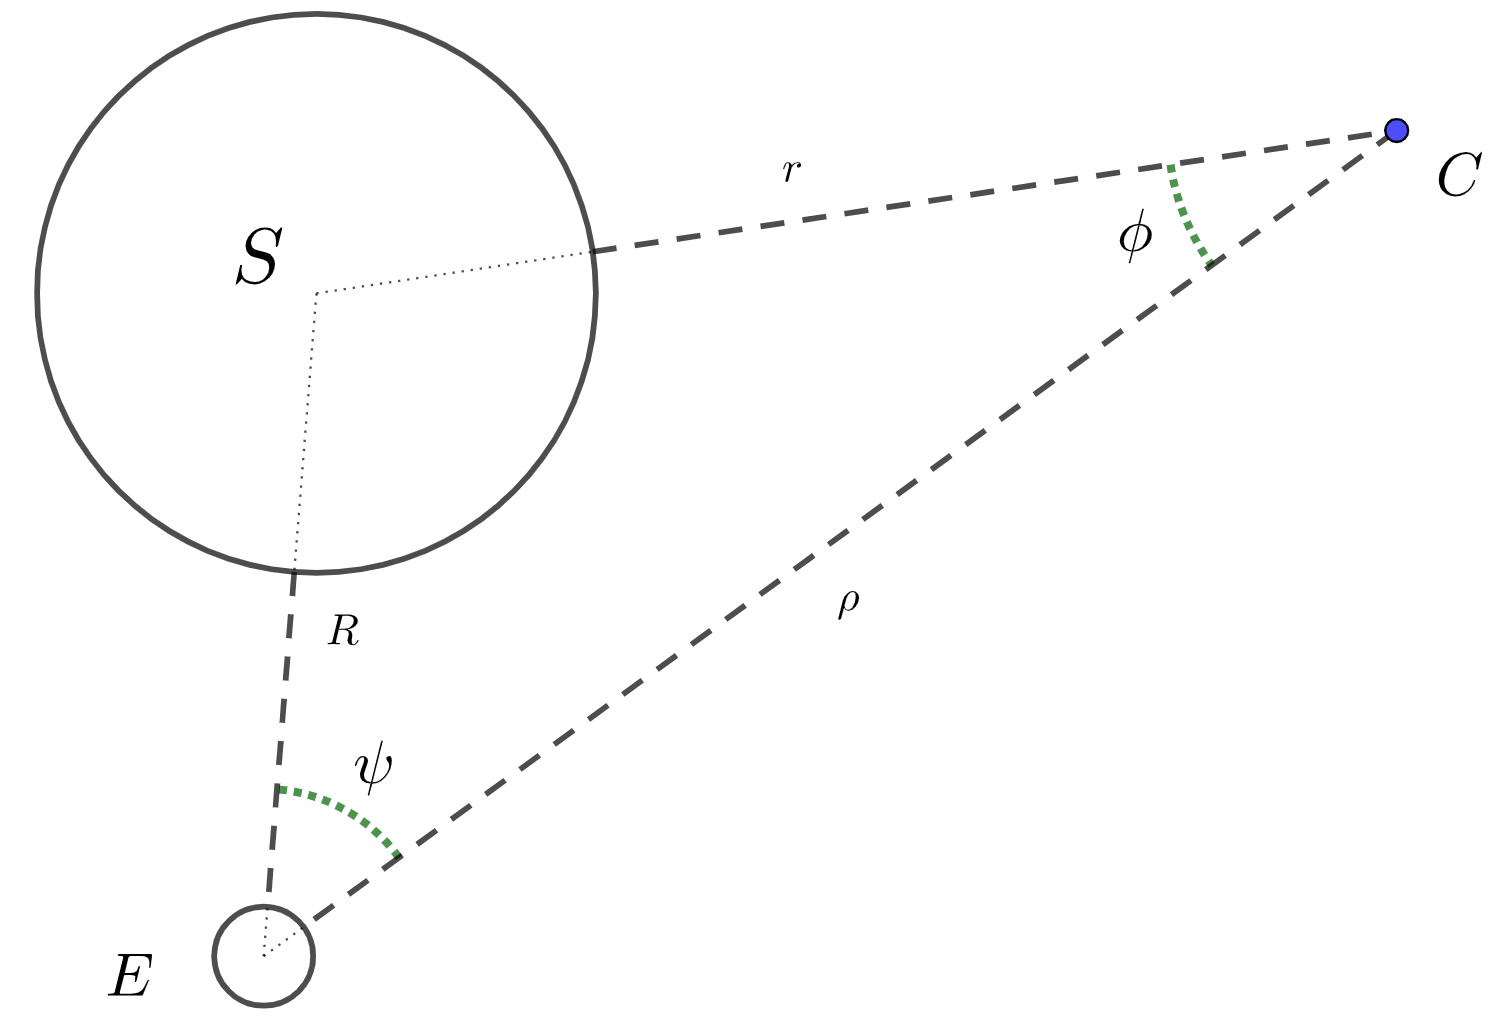
\includegraphics[scale=0.15]{images/notation_angles.png}
\caption{Triángulo formado por $S$, $E$ y $C$ junto a las distancias y ángulos generados.}
\label{fig:notation_angles}
\end{figure}

Nos encontramos ahora ante un problema de resolución de triángulos \cite{ASA}. A partir de la figura superior y del teorema de los senos ($\ddfrac{a}{\sin{\alpha}}=\ddfrac{b}{\sin{\beta}}=\ddfrac{c}{\sin{\gamma}}$), podemos escribir las siguientes ecuaciones:
\begin{align}
\left\{
\begin{array}{l}
	\rho=R\ddfrac{\sin{(\psi+\phi)}}{\sin{\phi}}\\
	r=R\ddfrac{\sin{\psi}}{\sin{\phi}}
\end{array}
\right.
\label{eq:triangle_relations_2}
\end{align}

Además, recordemos que podemos obtener el ángulo $\psi$ mediante:
\[
R\cos{\psi}=X\lambda+Y\mu+Z\nu\\
\]

\noindent obteniendo así que el valor de $\psi$ estará en el primer o cuarto cuadrante, pues $R>0$ y el producto escalar de $(X,Y,Z)$ por $(\lambda,\mu,\nu)$ es positivo. Pero, como nos encontramos en un triángulo, se ha de cumplir que $\psi<\pi$, y suponemos que el ángulo $\psi$ es agudo.\\

Si sustituimos las ecuaciones  \eqref{eq:triangle_relations_2} en la ecuación de $\rho$ en \eqref{eq:rho_values}, esta pasará a ser:
\[
R\sin{\psi}\cos{\phi}+\left(R\cos{\psi}-\ddfrac{D_1}{DR^3}\right)\sin{\phi}=\ddfrac{-D_1}{DR^3\sin^3{\psi}}\sin^4{\phi}
\]

\noindent de manera que, ya que podemos obtener el valor de $\psi$ utilizando la primera ecuación de \eqref{eq:triangle_relations_2}, nos queda una ecuación con una única incógnita, $\phi$.\\

Ahora, consideramos el vector en el plano $(R\cos{\psi}-\ddfrac{D_1}{DR^3},R\sin{\psi})$ y suponemos que es distinto del origen. Realmente esto ocurre siempre, ya que, como el ángulo $\psi$ es agudo y distinto de $0$, $R\sin{\psi}$ será distinto de $0$. Como consecuencia, al no ser el origen, podremos expresar dicho punto en coordenadas polares de la forma $N(\cos{m},\sin{m})$, con $N\neq0$ y pudiendo escoger el valor de $m$ en $(0,2\pi)$.\\

Con el fin de simplificar esta ecuación, definimos las siguientes expresiones:
\begin{align}
\left\{
\begin{array}{l}
	N\sin{m}=R\sin{\psi}\\
	N\cos{m}=R\cos{\psi}-\ddfrac{D_1}{DR^3}\\
	M=\ddfrac{-NDR^3\sin^3{\psi}}{D_1}
\end{array}
\right.
\label{eq:to_simplify}
\end{align}

Las dos primeras ecuaciones vienen dadas de la forma polar comentada anteriormente. Respecto a la tercera ecuación, la utilizaremos para darle un signo al valor $N$, de manera que podamos reducir el intervalo donde escoger el valor de $m$ a $(0,\pi)$. El signo de $N$ será elegido de tal manera que $M$ sea positivo, y como $\sin{\psi}>0$, $R>0$, el valor $N$ será positivo cuando $\ddfrac{D_1}{D}$ sea negativo y viceversa.\\

Hay ciertos casos excepcionales en las ecuaciones superiores. Si el término de la izquierda de la primera ecuación se anulase, llegaríamos a que $R\sin{\psi}=0$; como $R>0$ por definición, $\sin{\psi}=0$ y $\psi=k\pi$, $k\in\mathbb{Z}$, pero esta situación no es válida, pues entonces el sistema formado por el Sol, la Tierra y el objeto observado no formaría un triángulo tal y como queremos.\\

Fijado el signo de $M$, las dos primeras ecuaciones de \eqref{eq:to_simplify} determinarán unívocamente los valores $N$ y $m$, y la expresión que queríamos simplificar pasa a ser simplemente:
\begin{align}
\def\arraystretch{2}
\begin{array}{c}
	N\sin{m}\cos{\phi}+N\cos{m}\sin{\phi}=N\sin{(\phi+m)}=\ddfrac{N}{M}\sin^4{\phi} \Longrightarrow\\
	\Longrightarrow\sin^4{\phi}=M\sin{(\phi+m)}
\end{array}
\label{eq:phi_solution}
\end{align}

Aunque la ecuación \eqref{eq:phi_solution} podría estar definida para $\phi\in\mathbb{R}$, solo nos interesará en el intervalo $(0,\pi)$; es más, dicho intervalo se puede seguir reduciendo. Ya que $\phi$ es uno de los tres ángulos, y teniendo en cuenta cómo hemos definido $m$, podremos asegurar que $\phi=\pi-\psi$ es una solución válida (se puede comprobar sustituyendo en \eqref{eq:phi_solution}), aunque no es de valor práctico ya que que ésta corresponde a la posición del observador en la Tierra. Por tanto, dado que la solución ha de pertenecer al problema físico y que nos encontramos en un triángulo, podemos asegurar que:
\[
\phi<\pi-\psi
\]
\noindent y por tanto buscaremos una solución para la ecuación \eqref{eq:phi_solution}, no en todos los puntos que está definida, sino con $\phi$ estrictamente entre 0 y $\pi-\psi$.\\

Así, las soluciones de \eqref{eq:phi_solution} han de ser las intersecciones entre las curvas que definen las ecuaciones de la izquierda y de la derecha, es decir, la intersección entre:
\[
\left\{
\begin{array}{l}
	y_1=\sin^4{\phi}\\
	y_2=M\sin{(\phi+m)}
\end{array}
\right.
\]

Si el valor de $m$ es negativo cercano a cero y $M$ es ligeramente menor que 1, podemos ver la relación entre ambas curvas $y_1$, $y_2$ en la figura inferior:

\begin{figure}[H]
\centering
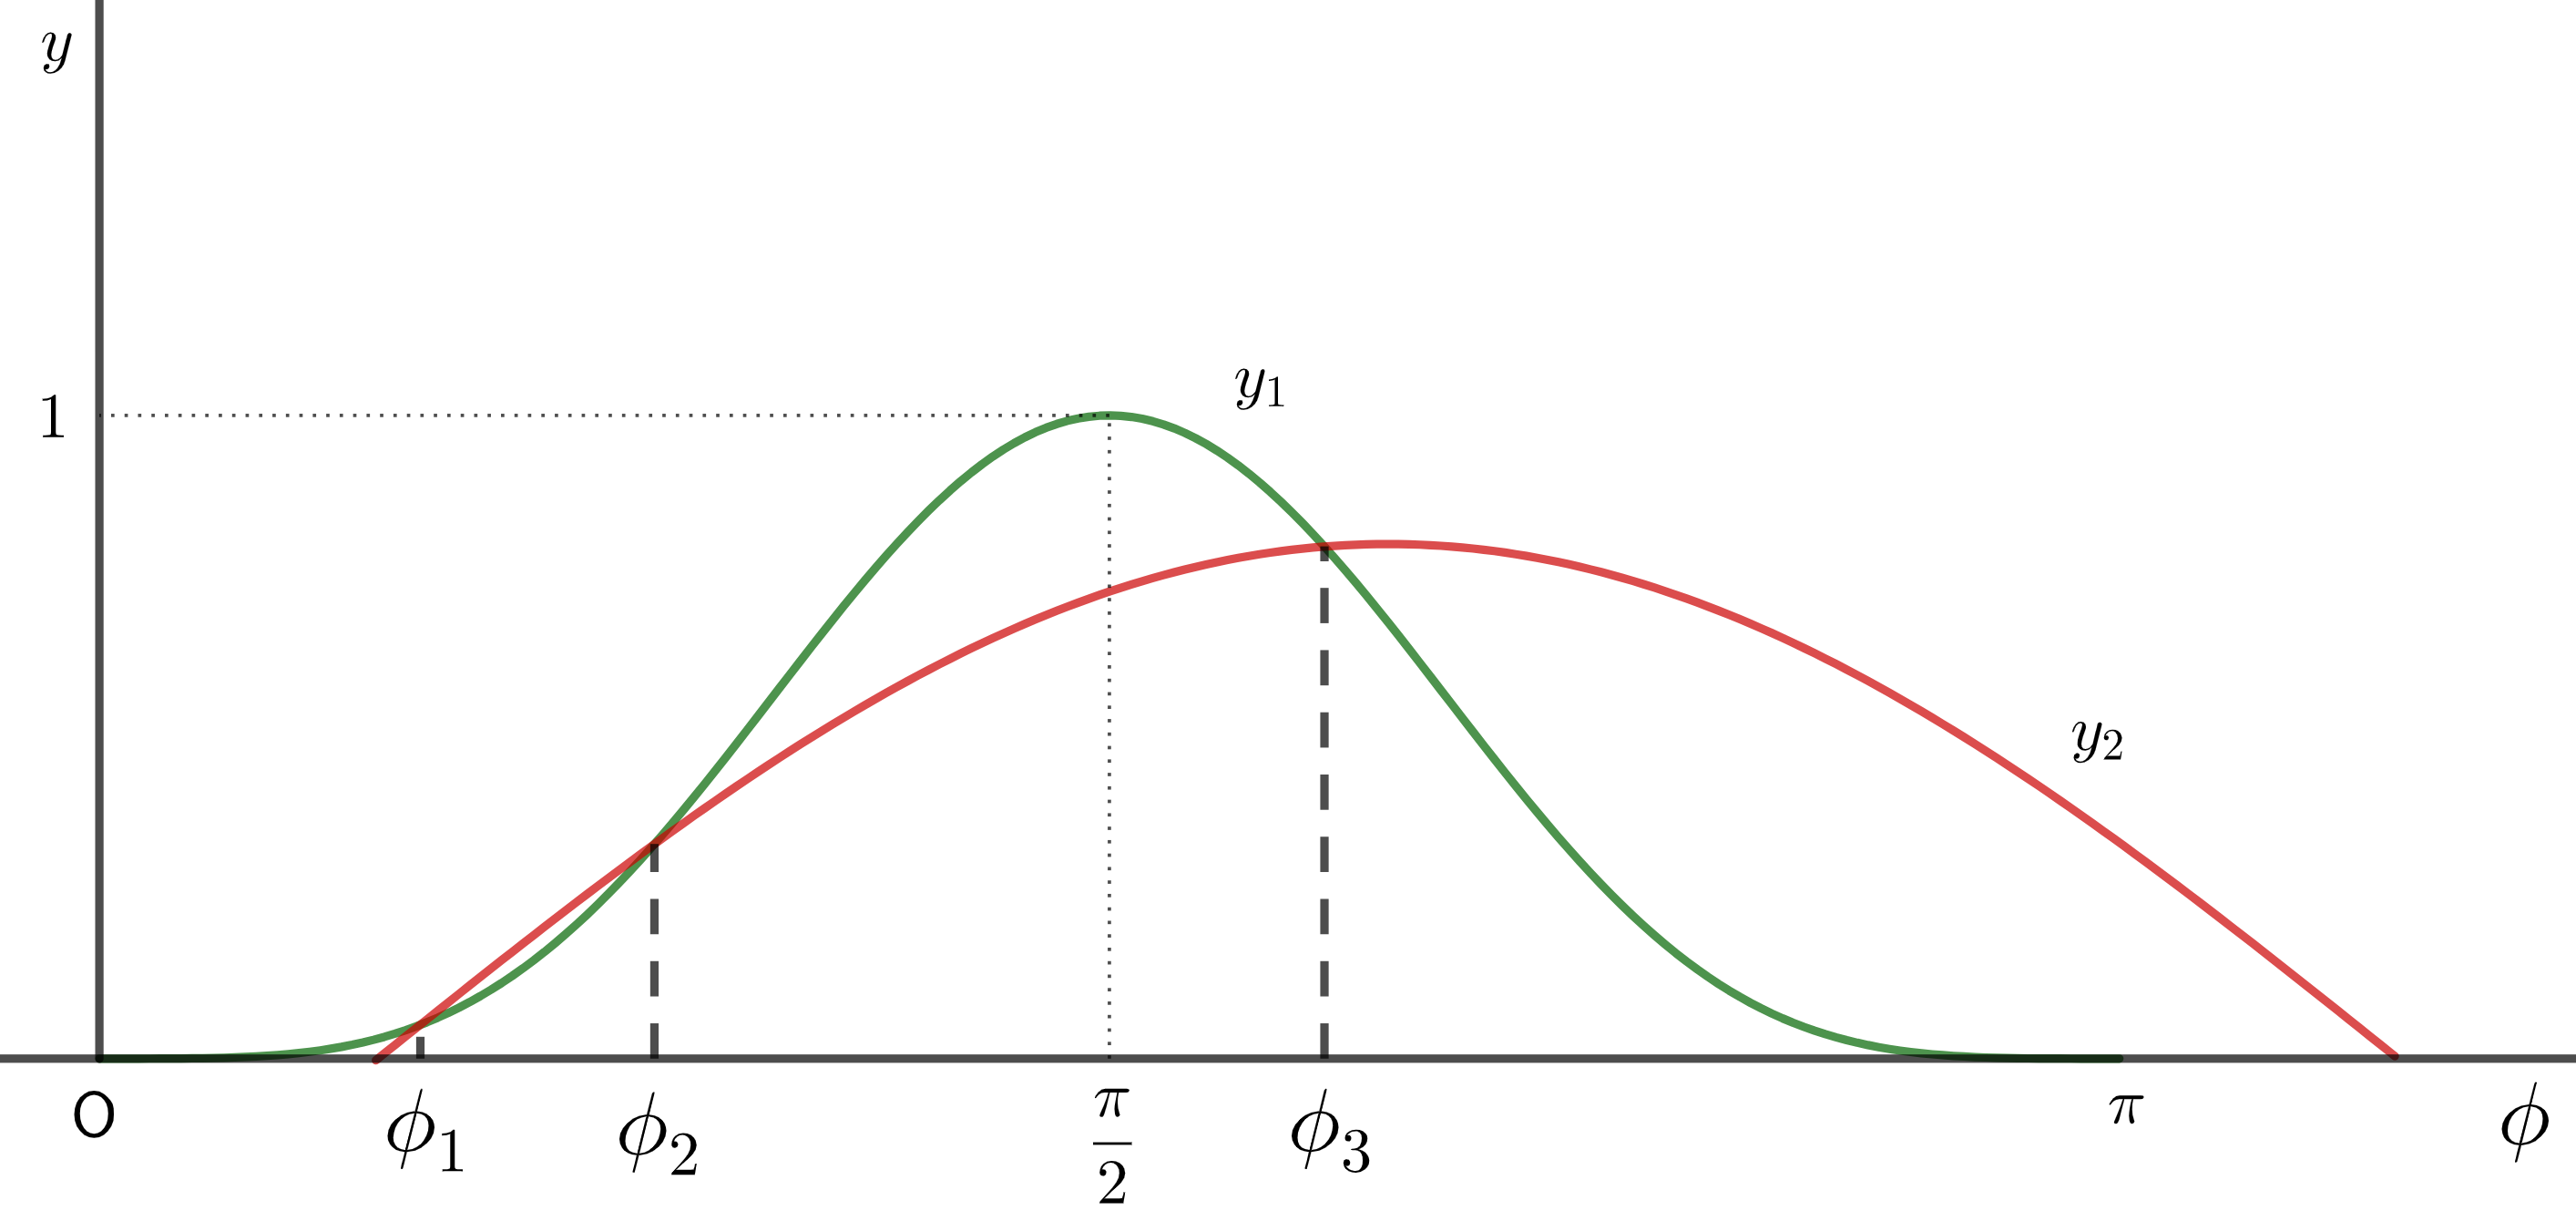
\includegraphics[scale=0.125]{images/phi_solution_m_negative_M_near_1.png}
\caption{Representación gráfica de $y_1$ e $y_2$ ($\frac{D_1}{D}>0$).}
\label{fig:phi_solution_m_negative_M_near_1}
\end{figure}

A partir de dicha imagen podemos observar que obtenemos tres intersecciones de las curvas, correspondientes cada una a una solución de \eqref{eq:phi_solution} y con $\phi_1<\phi_2<\phi_3$, sabiendo que una de ellas ha de ser $\pi-\psi$.\\

Discutamos ahora según el signo de $\frac{D_1}{D}$ los valores de $r$, $R$ y $m$. Comencemos considerando que $\frac{D_1}{D}$ es positivo. Es claro que $\rho$ y $r$ han de ser positivos, por lo que deducimos de la primera ecuación de \eqref{eq:rho_values} que $r$ ha de ser mayor que $R$. Por tanto, como $\psi$ ha de ser menor que 180º (pues estamos en un triángulo), utilizando las ecuaciones \eqref{eq:to_simplify} tenemos:
\[
\def\arraystretch{2}
\begin{array}{l}
M=\ddfrac{-NDR^3\sin^3{\psi}}{D_1}>0 \Longrightarrow N<0 \\
R\sin{\psi}>0 \Longrightarrow N\sin{m}>0 \Longrightarrow \sin{m}<0 \Longrightarrow m\in(\pi,2\pi)
\end{array}
\]

Por tanto, $N$ es negativo y $m$ estará en el tercer o cuarto cuadrante.\\

Si $m$ está en el cuarto cuadrante, la rama ascendente de la curva $y_2$ atraviesa el eje de abscisas $\phi$ en el primer cuadrante y, si $M<1$, las relaciones entre las dos curvas serán las que podemos ver en la figura \ref{fig:phi_solution_m_negative_M_near_1}. Si el valor de $m$ es cercano a 180º tendremos tres soluciones disponibles $\phi_1$, $\phi_2$, $\phi_3$, una de las cuales corresponderá al observador ($\phi_i=\pi-\psi$). Discutamos según cuál de las tres soluciones toma este valor:
\begin{itemize}
\item Si $\phi_1=\pi-\psi$, entonces el problema no tendría solución dado que cualquiera de las otras dos soluciones sería mayor que $\pi-\psi$.
\item Si $\phi_2=\pi-\psi$, se sigue del hecho de que $\phi<\pi-\psi$ que la solución ha de ser $\phi_1$ y es única.
\item Si $\phi_3=\pi-\psi$, las otras dos soluciones cumplirán todas las condiciones del problema, no pudiendo determinar cuál de las dos pertenece a la órbita real del cuerpo observado (siempre que no tengamos información adicional). Si tuviéramos una cuarta medición, repetiríamos el proceso anterior eliminando una de las mediciones tomadas y añadiendo ésta nueva; la solución que se repita (aproximadamente) será la perteneciente al problema real.

Pero, si solo dispusiésemos de tres mediciones, podría darse el caso de que los valores de $r$ y $\rho$ proporcionados por la solución $\phi_1$ fueran demasiado grandes como para que el objeto fuera visible para el observador, llegando así a la conclusión de que $\phi_2$, el cuál proporcionaría un $r$ más pequeño, pertenecería al problema físico.
\end{itemize} 

A medida que la rama ascendente de la curva $y_2$ se mueve hacia la derecha, es decir, fijando $M$ hacemos decrecer $m$, las soluciones $\phi_1$ y $\phi_2$ tienden a coincidir, y en estas condiciones el problema no tendría solución. Por tanto:
\begin{quote}
\textit{Si $\frac{D_1}{D}>0$, la distancia $r$ es mayor que $R$, el ángulo $m$ estará en el cuarto cuadrante y disponemos de una o dos soluciones del problema físico en función de que $\phi_2$ o $\phi_3$ sea igual a $\pi-\psi$.}\\
\end{quote}

Veamos ahora el caso contrario. 

\begin{figure}[H]
\centering
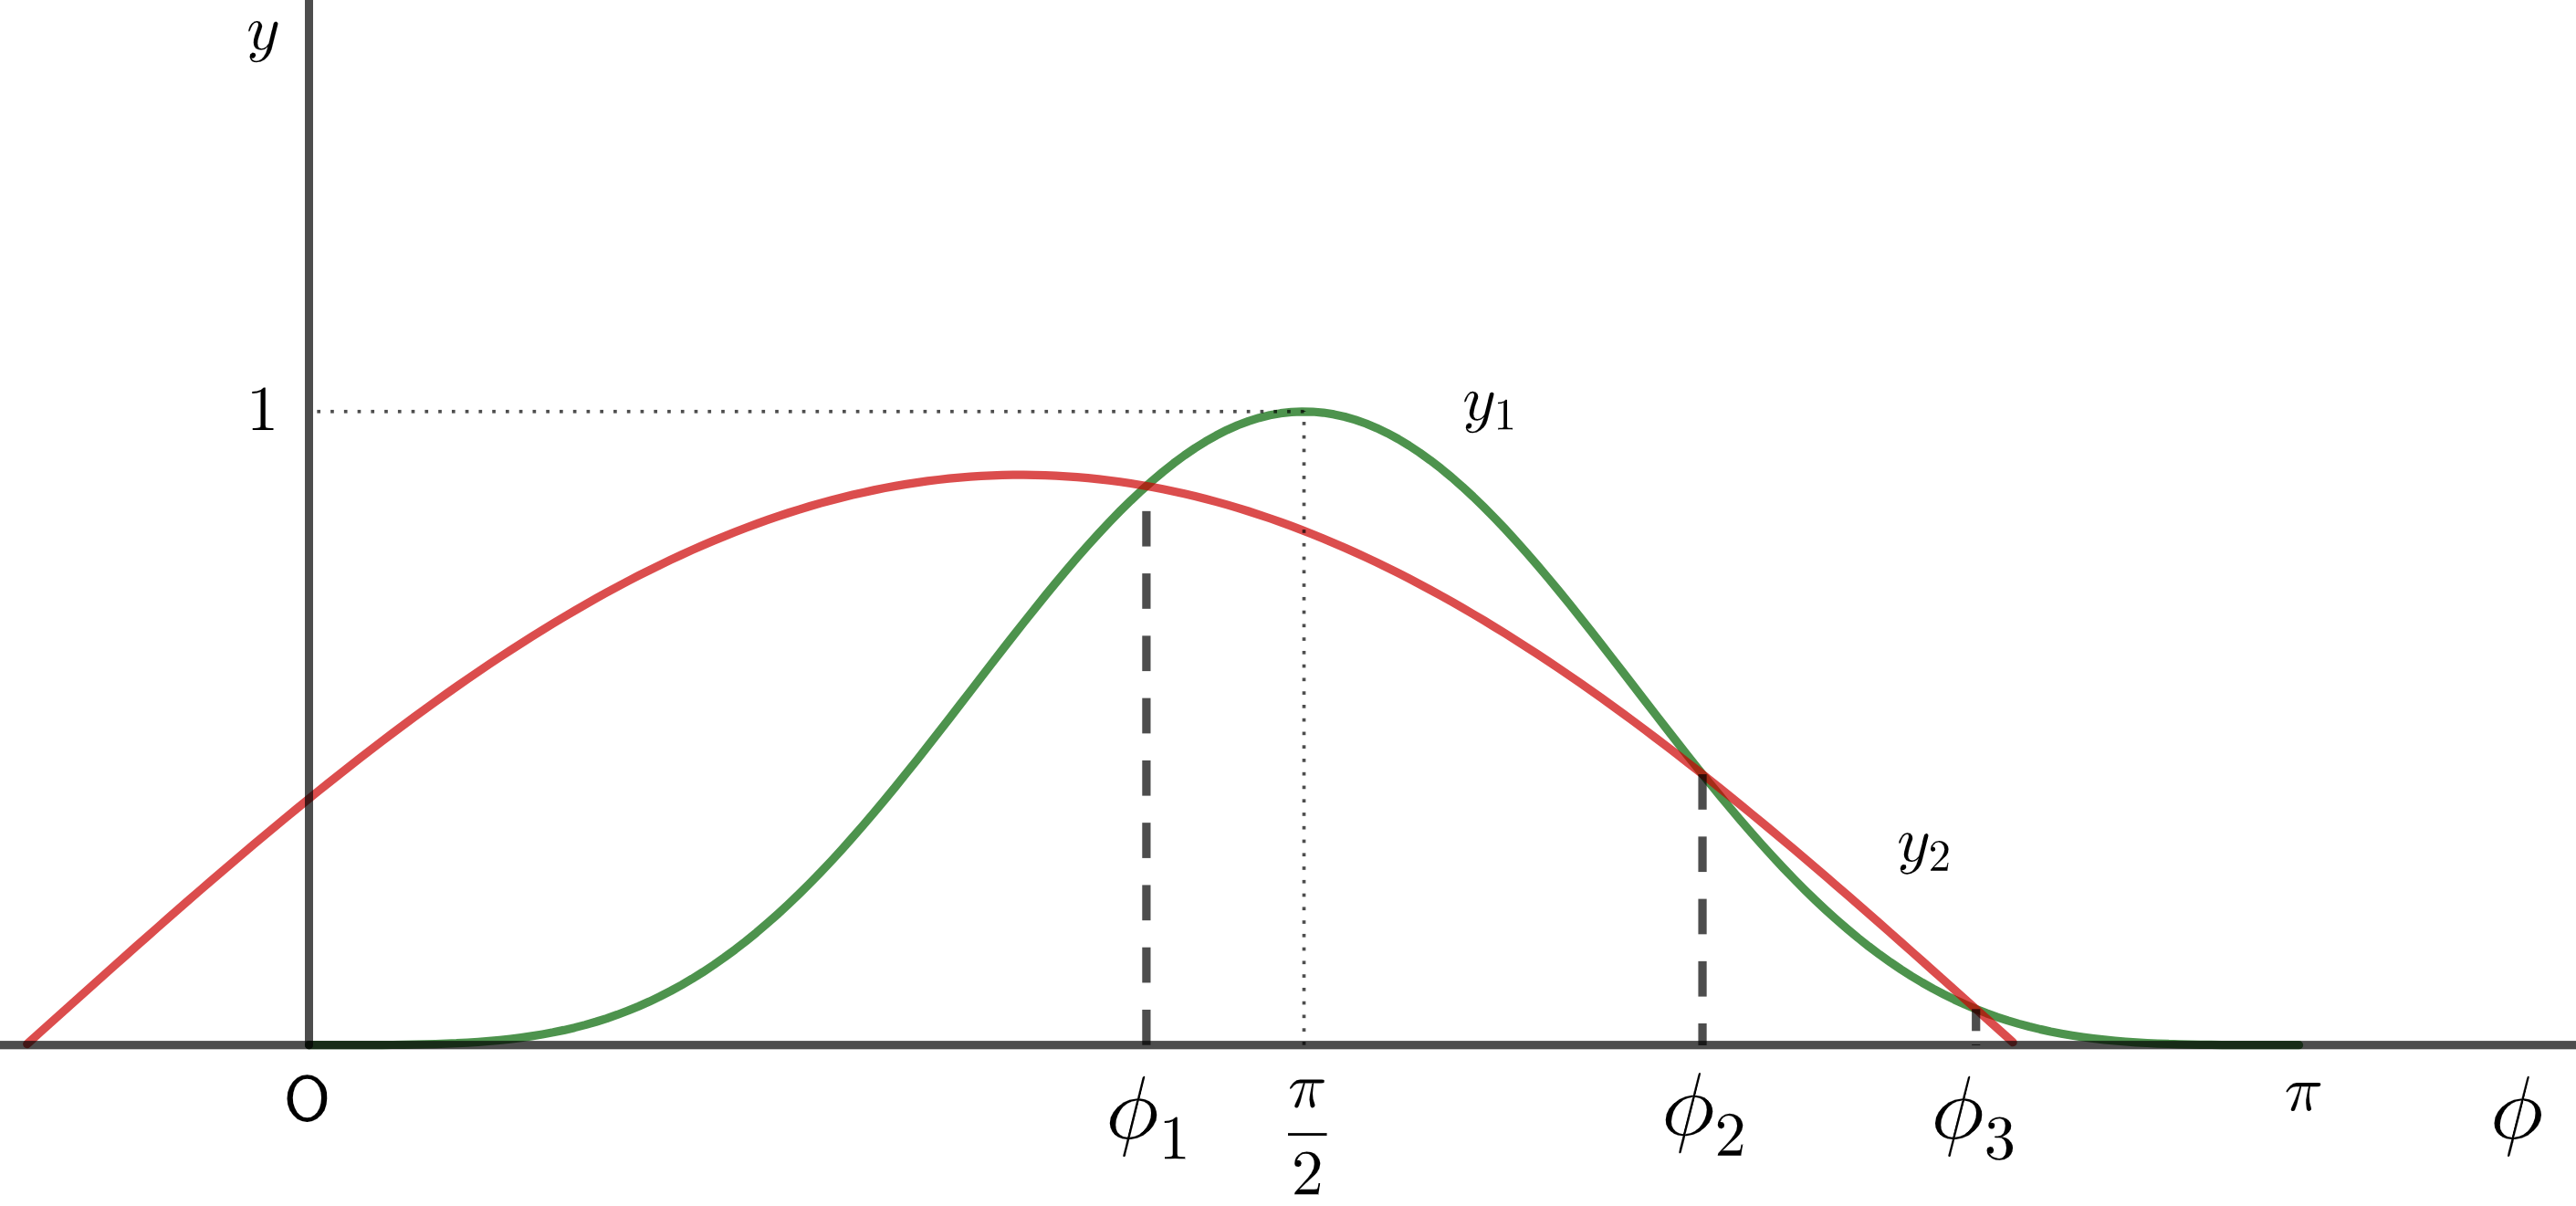
\includegraphics[scale=0.125]{images/phi_solution_m_positive_M_near_1.png}
\caption{Representación gráfica de $y_1$ e $y_2$ ($\frac{D_1}{D}<0$).}
\label{fig:phi_solution_m_positive_M_near_1}
\end{figure}

Supongamos que $\frac{D_1}{D}$ es negativo, de tal manera que, procediendo como en el caso positivo, llegamos a que $r<R$ y que $m$ está en el primer o segundo cuadrante. Si $m$ está en el primer cuadrante, la rama descendente de la curva $y_2$ atraviesa el eje de abscisas $\phi$ en el segundo cuadrante, y para un $m$ pequeño y $M<1$, las relaciones entre las dos curvas serán las que podemos ver en la gráfica \ref{fig:phi_solution_m_positive_M_near_1}. En este caso, la solución será única o doble en función de que $\phi_2$ o $\phi_3$ valgan $\pi-\psi$. Por último, si $m$ estuviera en el segundo cuadrante, la rama descendente de $y_2$ cortaría el eje de abscisas en el primer cuadrante, por lo que $\phi_2$ y $\phi_3$ no serían reales y el problema no tendría solución. Así, tenemos que:
\begin{quote}
\textit{Si $\frac{D_1}{D}<0$, la distancia $r$ es menor que $R$, el ángulo $m$ estará en el primer cuadrante y disponemos de una o dos soluciones del problema físico en función de que $\phi_2$ o $\phi_3$ sea igual a $\pi-\psi$.}\\
\end{quote}

Como consecuencia de toda esta discusión concluimos que, en determinadas situaciones, según las medidas que se nos den y el número de estas, nos encontraremos ante una única respuesta o dos respuestas, y en este segundo caso tendremos que discernir sobre cuál de las dos soluciones pertenecerá al problema físico. \cite{moulton}\\

%%%%%%%%%%%%%%%%%%%%%%%%%%%%%%%%

%%%%%%%%%%%%%%%%%%%%%%%%%%%%%%%%
\section{Aproximación numérica mediante el método de Newton.}
\label{sec:newton_rhapson}
Tras haber realizado un estudio teórico de la ecuación \eqref{eq:phi_solution}, pasemos a buscar un método de resolución para ésta. Dado que no podemos encontrar valores exactos de $\phi$ que satisfagan la ecuación, pues no hay una fórmula explícita para la solución, utilizaremos el método de Newton para obtener un valor aproximado.\\

Considerando una función $f$ derivable y $x_0$ un valor inicial, definimos el método de Newton para cada $n$ como:
\[
x_{n+1}=x_n-\ddfrac{f(x_n)}{f'(x_n)}, n\geq0
\]

Para no aplicar la operación superior de forma infinita, impondremos una tolerancia $\delta$ a la hora de aplicar el método de manera que cuando $|x_{k+1}-x_k|<\delta$, la solución será $x_{k+1}$. Es necesario que $f'(x)\neq0$ para poder llevar este método a la práctica.\\

En nuestro caso, tomando $f(x)=\sin^4{x}-M\sin{(x+m)}$, tenemos que su derivada será $f'(x)=4\sin^3{x}\cos{x}-M\cos{(x+m)}$ de manera que la sucesión para la aproximación mediante el método de Newton será:
\begin{align}
x_{n+1}=x_n-\ddfrac{\sin^4{x_n}-M\sin{(x_n+m)}}{4\sin^3{x_n}\cos{x_n}-M\cos{(x_n+m)}}, \; \; \; \; \; n\geq0
\label{eq:phi_newton}
\end{align}

El método de Newton no siempre es convergente, por lo que es conveniente mencionar los teoremas de convergencia de este método. 
\begin{theorem}
\label{theo:convergence_newton}
Sea $f:I\rightarrow\mathbb{R}$ una función de clase 2 en un intervalo abierto $I$. Supongamos que existe $x^*$ tal que $f(x^*)=0$ y $f'(x^*)\neq0$; entonces, existe $\varepsilon>0$ tal que si $x_0\in[x^*-\varepsilon,x^*+\varepsilon]$, el método de Newton permite definir la sucesión $\{x_n\}_{n\in\mathbb{N}}$ que converge a $x^*$. Además, cuando $f''(x^*)\neq0$, dicha sucesión tiene orden de convergencia 2. \cite{MNII}\\
\end{theorem}

Dado que la función que queremos aproximar con el método de Newton es infinito-derivable por ser una función trigonométrica, podremos aplicar el teorema superior encontrado así el valor de $\phi$ para el que se cumple la ecuación \eqref{eq:phi_solution}.\\

Notemos que este teorema solo nos garantiza la convergencia supuesto que el punto $x_0$ sea cercano a la raíz, por lo que será buena idea separar las raíces por Bolzano y elegir el valor intermedio de los intervalos obtenidos como valor inicial para aplicar el método de Newton. La separación de raíces consiste en escoger un número adecuado de puntos $\alpha_1,...,\alpha_k\in[a,b]$ y aplicar el teorema de Bolzano para cada par $(\alpha_j,\alpha_{j+1})$, acotando así los intervalos donde buscar las raíces de una función. Ya que en nuestro caso buscamos la solución en el intervalo $[0,\pi]$ podremos escoger los puntos de la manera $\frac{j\cdot \pi}{n}$, con $j=0,...,n$, y una vez acotemos la raíz quedarnos como valor inicial:
\[
x_0=\ddfrac{\ddfrac{j\cdot\pi}{n}+\ddfrac{(j+1)\cdot\pi}{n}}{2}=\ddfrac{(2j+1)\cdot\pi}{2n}
\]

Veamos ahora un caso práctico de la aplicación de este método para determinar las soluciones de \eqref{eq:phi_solution}. Tomemos $M=0.6$ y $m=6$, por lo que $m$ estará en el cuarto cuadrante y nos encontraremos en el caso de \ref{fig:phi_solution_m_negative_M_near_1}. Escojamos $n=8$ y separemos las raíces en intervalos para escoger el valor de $x_0$.
\begin{table}[H]
\centering
\resizebox{9.5cm}{!}{%
\begin{tabular}{c|c|c|c|c|c|c|c|c|c}
$\alpha_j$    & $0$ & $\frac{\pi}{8}$ & $\frac{\pi}{4}$ & $\frac{3\pi}{8}$ & $\frac{\pi}{2}$ & $\frac{5\pi}{8}$ & $\frac{3\pi}{4}$ & $\frac{7\pi}{8}$ & $\pi$ \\ \hline
$f(\alpha_j)$ & + & -             & -             & +              & +             & +              & -              & -              & -  
\end{tabular}%
}
\end{table}

Tomamos, por ejemplo, el intervalo $[0,\frac{\pi}{8}]$ en el que nuestra función cambia de signo entre sus extremos. Calculamos el valor medio del intervalo, lo elegimos como valor inicial, $x_0=\frac{\pi}{16}$, y aplicamos el método de Newton con una tolerancia de $10^{-5}$. Veamos en una tabla cómo va convergiendo la solución.
\begin{table}[H]
\centering
\def\arraystretch{1.5}
\setlength{\tabcolsep}{20pt}
\begin{tabular}{cc|c}
      &                       & $x_i-x_{i-1}$                   \\ \hline
$x_0$ & $\pi/16$              &                                 \\ \hline
$x_1$ & $0.2904116552751586$  & $0.0940621144257965$            \\ \hline
$x_2$ & $0.295092645742656$   & $0.00468099046749737$           \\ \hline
$x_3$ & $0.29511191583666796$ & $1.92700940119805\cdot10^{-5}$  \\ \hline
$x_4$ & $0.29511191616986304$ & $3.33195082635740\cdot10^{-10}$ \\ \hline
\end{tabular}
\end{table}

Por tanto, en cuatro iteraciones del método la diferencia entre las soluciones obtenidas es menor a la tolerancia que hemos fijado, obteniendo así que $\phi_1=0.29511191616986304$ es una solución de \eqref{eq:phi_solution}. De la misma manera calcularemos las raíces $\phi_2$ en $[\frac{\pi}{4},\frac{3\pi}{8}]$ y $\phi_3$ en $[\frac{5\pi}{8},\frac{3\pi}{4}]$.\\

Tras aplicar el método de Newton y haber obtenido todas las soluciones de \eqref{eq:phi_solution} en el intervalo $[0,\pi]$, nos faltará comprobar cuál de las soluciones obtenidas es igual a $\pi-\psi$, pudiendo determinar así si hay o no unicidad para el problema físico. Aún así, es posible determinar la unicidad de la solución sin necesidad de resolver la ecuación \eqref{eq:phi_solution}, como veremos a continuación.\\

\section{Unicidad de la solución.}
\label{sec:unicidad}
Tal y como hemos visto en la sección anterior, la solución del problema físico será única si $\phi_2=\pi-\psi$, independientemente del signo de $\frac{D_1}{D}$; en otro caso, la solución será doble o no existirá.\\

Fijémonos en la figura \ref{fig:phi_solution_m_negative_M_near_1}, donde aparecen tres intersecciones entre las curvas $y_1$ e $y_2$. La observación fundamental en esta gráfica reside en el hecho de que $\phi_2$ es un cero positivo, entendiendo por esto que la derivada en dicho punto es positiva, es decir, la función es creciente, y $\phi_1$ y $\phi_3$ son ceros negativos, la función decrece. Podemos ver esto más fácilmente en la siguiente imagen:

\begin{figure}[H]
\centering
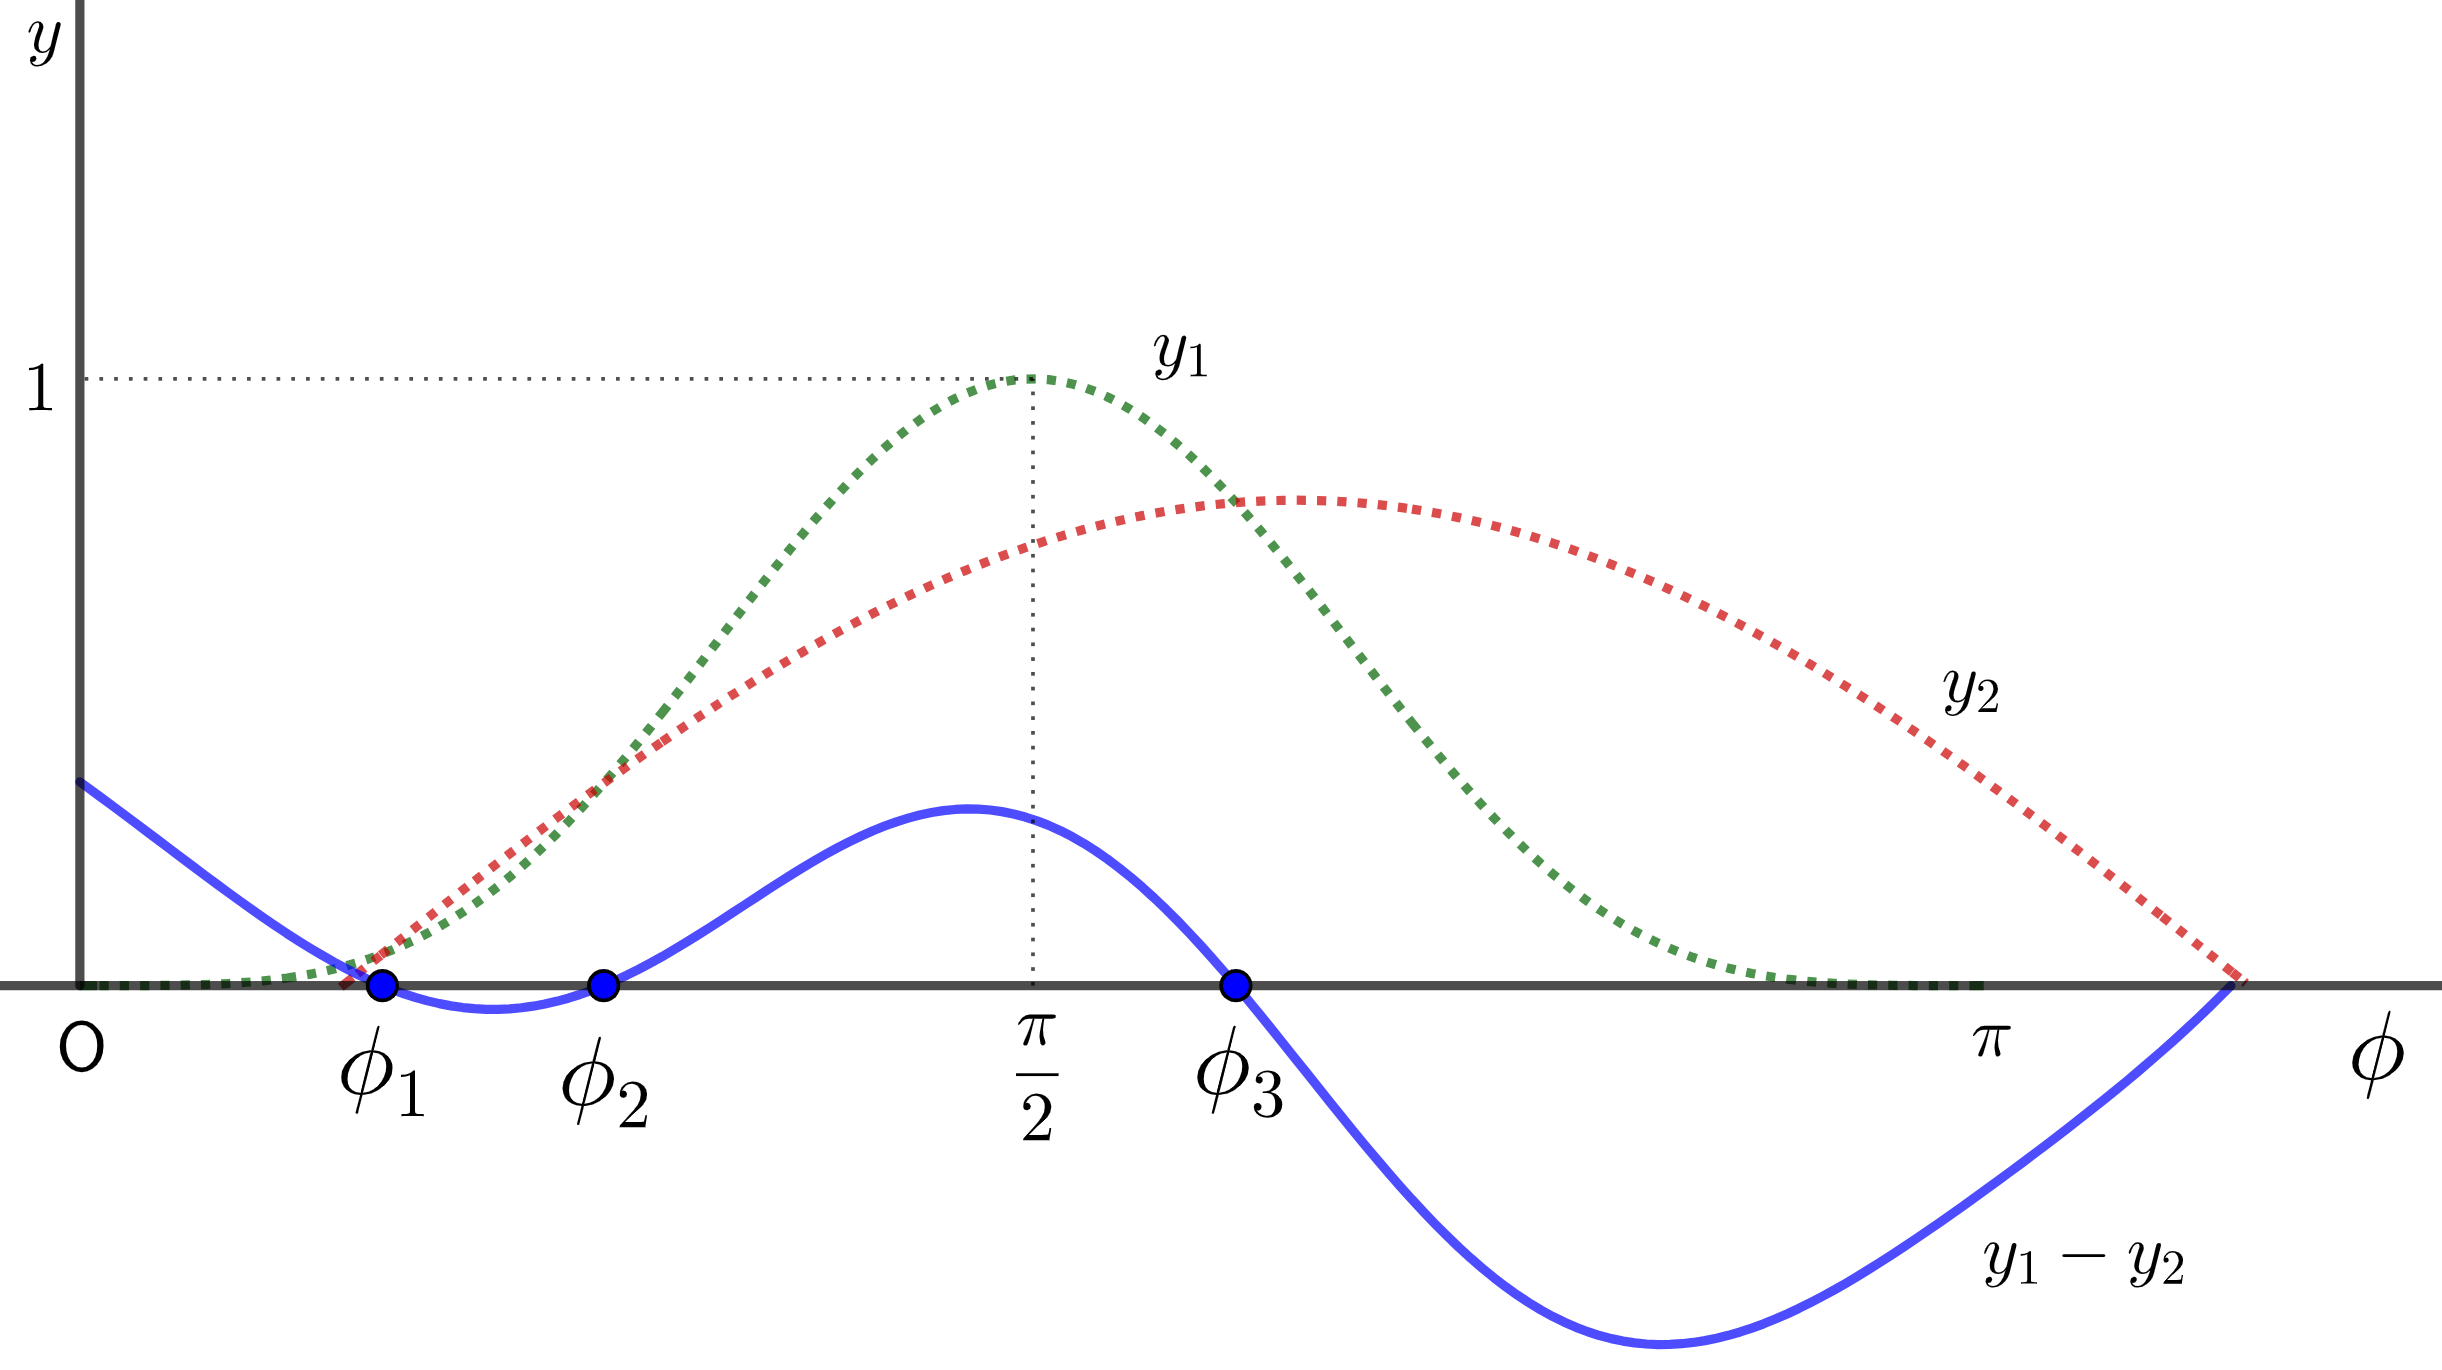
\includegraphics[scale=0.125]{images/y_1_menos_y_2.png}
\caption{Representación gráfica de $y_1-y_2$ cuando $\ddfrac{D_1}{D}>0$.}
\label{fig:y_1_menos_y_2}
\end{figure}

Por otra parte, calculemos la derivada de $y_1-y_2$:
\[
(y_1-y_2)'(x)=4\sin^3{\phi}\cos{\phi}-M\cos{(\phi+m)}
\]

Pues bien, para que nuestra solución sea única tendrá que cumplirse que $\phi_2=\pi-\psi$, y esto quiere decir que la derivada de $y_1-y_2$ en el punto $\pi-\psi$ ha de ser positiva. Desarrollemos la derivada en este punto para comprobar más fácilmente en qué casos se cumple la unicidad.
\[
\def\arraystretch{2}
\begin{array}{ll}
  & 4\sin^3{(\pi-\psi)}\cos{(\pi-\psi)}-M\cos{(\pi-\psi+m)}=\\
= &-4\sin^3{(\pi-\psi)}\cos{\psi}+M\cos{(-\psi+m)}=\\
= & \left[\ddfrac{4MD_1}{NDR^3}\cos{\psi}+M(\cos{\psi}\cos{m}+\sin{\psi}\sin{m})\right]=\\
= & \ddfrac{4MD_1}{NDR^3}\cos{\psi}+M\left(\ddfrac{R\cos^2{\psi}}{N}-\ddfrac{D_1\cos{\psi}}{NDR^3}+\ddfrac{R\sin^2{\psi}}{N}\right)=\\
= & \ddfrac{4MD_1}{NDR^3}\cos{\psi}-\ddfrac{MD_1}{NDR^3}\cos{\psi}+\ddfrac{MR}{N}(\cos^2{\psi}+\sin^2{\psi})=\\
= & \ddfrac{MR}{N}\left(1+\ddfrac{3D_1}{DR^4}\cos{\psi}\right)
\end{array}
\]

Dado que $M$ y $R$ son valores positivos podremos obviarlos a la hora de escribir la desigualdad. Así, tenemos una condición de unicidad para el caso de la figura \ref{fig:phi_solution_m_negative_M_near_1}, es decir, cuando $\ddfrac{D_1}{D}$ sea positivo, facilitando así un estudio previo en la determinación del ángulo $\phi$.\\

El razonamiento para $\ddfrac{D_1}{D}<0$ es análogo; en este caso, $\phi_2$ será un cero negativo y las otras dos soluciones serán ceros positivos, por lo que tendremos que comprobar que la derivada en $\pi-\psi$ sea negativa.\\

Así, con las dos desigualdades que hemos obtenido, llegamos a la conclusión de que la condición para que el problema físico tenga solución única es:
\begin{align}
\left\{
\def\arraystretch{2}
\begin{array}{l}
	\ddfrac{1}{N}\left[1+\ddfrac{3D_1}{DR^4}\cos{\psi}\right]>0 \; \; \; \; \text{si} \; \; \; \; \ddfrac{D_1}{D}>0\\
	\ddfrac{1}{N}\left[1+\ddfrac{3D_1}{DR^4}\cos{\psi}\right]<0 \; \; \; \; \text{si} \; \; \; \; \ddfrac{D_1}{D}<0
\end{array}
\right.
\label{eq:condicion_unicidad}
\end{align}

Dado que todos los valores de estas ecuaciones están dados por simples observaciones, no será necesario resolver la ecuación \eqref{eq:phi_solution} para determinar la unicidad de la solución.\\

Sabemos que $N\neq0$, y por tanto el límite de las dos desigualdades será:
\[
\left[1+\ddfrac{3D_1}{DR^4}\cos{\psi}\right]=0
\]

Ahora, utilicemos \eqref{eq:rho_values} y la relación \eqref{eq:triangle_relations_1} para eliminar $\cos{\psi}$ y $\frac{D_1}{D}$ de la expresión superior.
\[
\left\{
\def\arraystretch{2}
\begin{array}{l}
	\cos{\psi}=\ddfrac{r^2-\rho^2-R^2}{-2\rho R}\\
	\ddfrac{D_1}{D}=\ddfrac{\rho}{\left(\ddfrac{1}{R^3}-\ddfrac{1}{r^3}\right)}
\end{array}
\right.
\]
\[
\def\arraystretch{2}
\begin{array}{ll}
& 1+\ddfrac{3}{R^4}\ddfrac{\rho}{\left(\ddfrac{1}{R^3}-\ddfrac{1}{r^3}\right)}\ddfrac{r^2-\rho^2-R^2}{-2\rho R}=0\\
\Longrightarrow & \ddfrac{3\rho}{\left(\ddfrac{1}{R^3}-\ddfrac{1}{r^3}\right)}(r^2-\rho^2-R^2)=2\rho R^5\\
\Longrightarrow & r^2-\rho^2-R^2=\ddfrac{2}{3}R^5\left(\ddfrac{1}{R^3}-\ddfrac{1}{r^3}\right)
\end{array}
\]

Obtenemos así la igualdad:
\begin{align}
\rho^2=r^2+\ddfrac{2}{3}\ddfrac{R^5}{r^3}-\ddfrac{5}{3}R^2
\label{eq:rho_cuadrado}
\end{align}

Tomemos el miembro de la derecha de esta igualdad como una ecuación en $r$ y calculemos sus extremos mediante el método clásico:
\[
\ddfrac{\partial}{\partial r} (r^2+\ddfrac{2}{3}\ddfrac{R^5}{r^3}-\ddfrac{5}{3}R^2)=2r-\ddfrac{2R^5}{r}=0 \Longrightarrow R=r
\]

Por tanto, tenemos un extremo en $r=R$, que comprobaremos si es máximo o mínimo derivando una vez más:
\[
\ddfrac{\partial^2}{\partial r^2}(r^2+\ddfrac{2}{3}\ddfrac{R^5}{r^3}-\ddfrac{5}{3}R^2)=\ddfrac{8R^5}{r^5}+2
 \; \; \; \xRightarrow[]{r=R} \; \; \; \ddfrac{8R^5}{R^5}+2>0, \; \; \; \forall R>0
\]

Así, tenemos un mínimo para nuestra función en $r=R$, y dado que el mínimo valor que puede tomar $R$ es cero, el miembro de la derecha de \eqref{eq:rho_cuadrado} alcanzará el mínimo en $r=0$, por lo que para cada valor de $r$ habrá un único valor positivo de $\rho$. Además, dado que estamos trabajando con el límite de las desigualdades \eqref{eq:condicion_unicidad}, todos los pares de valores $(\rho,r)$ que satisfagan la igualdad \eqref{eq:rho_cuadrado} se encontrarán en el límite de las regiones donde la solución es única, las cuales son superficies de revolución alrededor de la línea imaginaria que une la Tierra y el Sol. Intentemos entender esto mejor mediante una imagen.
\begin{figure}[H]
\centering
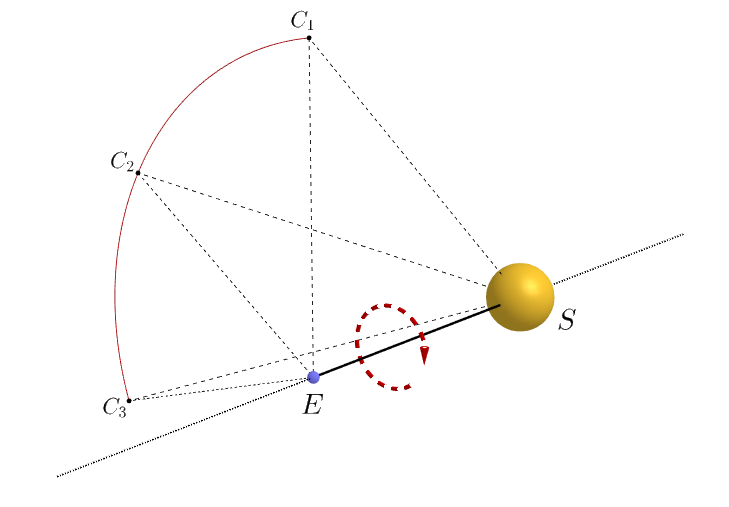
\includegraphics[scale=0.4]{images/eje_rotacion.png}
\caption{Distintas posiciones del cuerpo $C$, todas con las mismas distancias, $r$ y $\rho$, desde éstas al Sol y la Tierra.}
\label{fig:eje_rotacion}
\end{figure}

Dado que $r$ y $\rho$ son distancias del Sol y la Tierra al cuerpo observado, habrá infinitos puntos en el espacio tridimensional donde estos valores se mantengan. En la imagen superior podemos ver como, girando en torno a un círculo cuyo eje es el vector $\overrightarrow{SE}$, la distancia de cada $C_i$ es la misma independientemente de en qué punto del círculo se encuentre. Por tanto, volviendo a lo comentado anteriormente, podremos formar una superficie de revolución para el límite de las regiones donde la solución pasa a ser única tomando los pares $(\rho,r)$ en dicho límite y girando alrededor de vector $\overrightarrow{SE}$.

\begin{figure}[H]
\centering
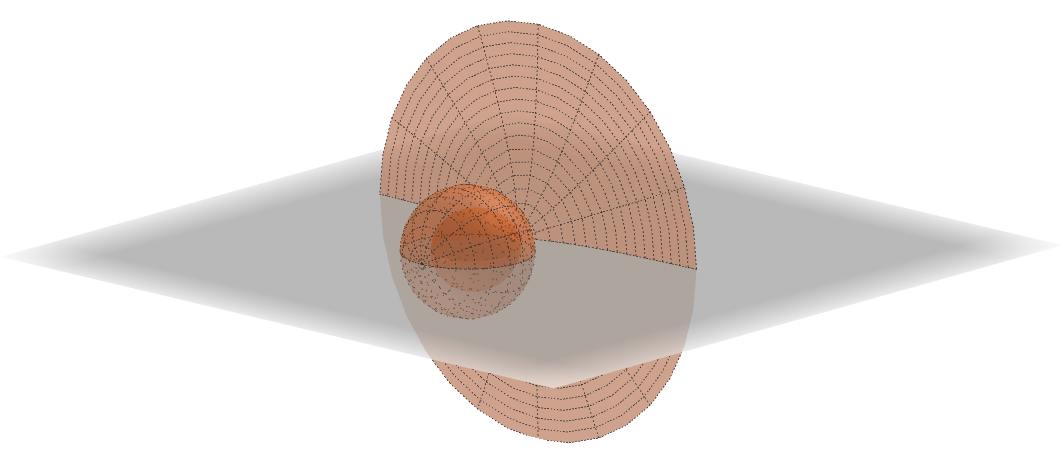
\includegraphics[scale=0.35]{images/sup_revol.png}
\caption{Superficie formada por los límites donde cambia la unicidad de la solución.}
\label{fig:sup_revol}
\end{figure}

En la imagen superior el círculo grande se extenderá hasta el infinito.\\

A continuación, para obtener una imagen más visual en la que estudiar el cambio en la unicidad de la solución al atravesar las regiones límite, representamos una sección de la superficie con un plano que pase por la recta $SE$.
\begin{figure}[H]
\centering
\subfloat{
	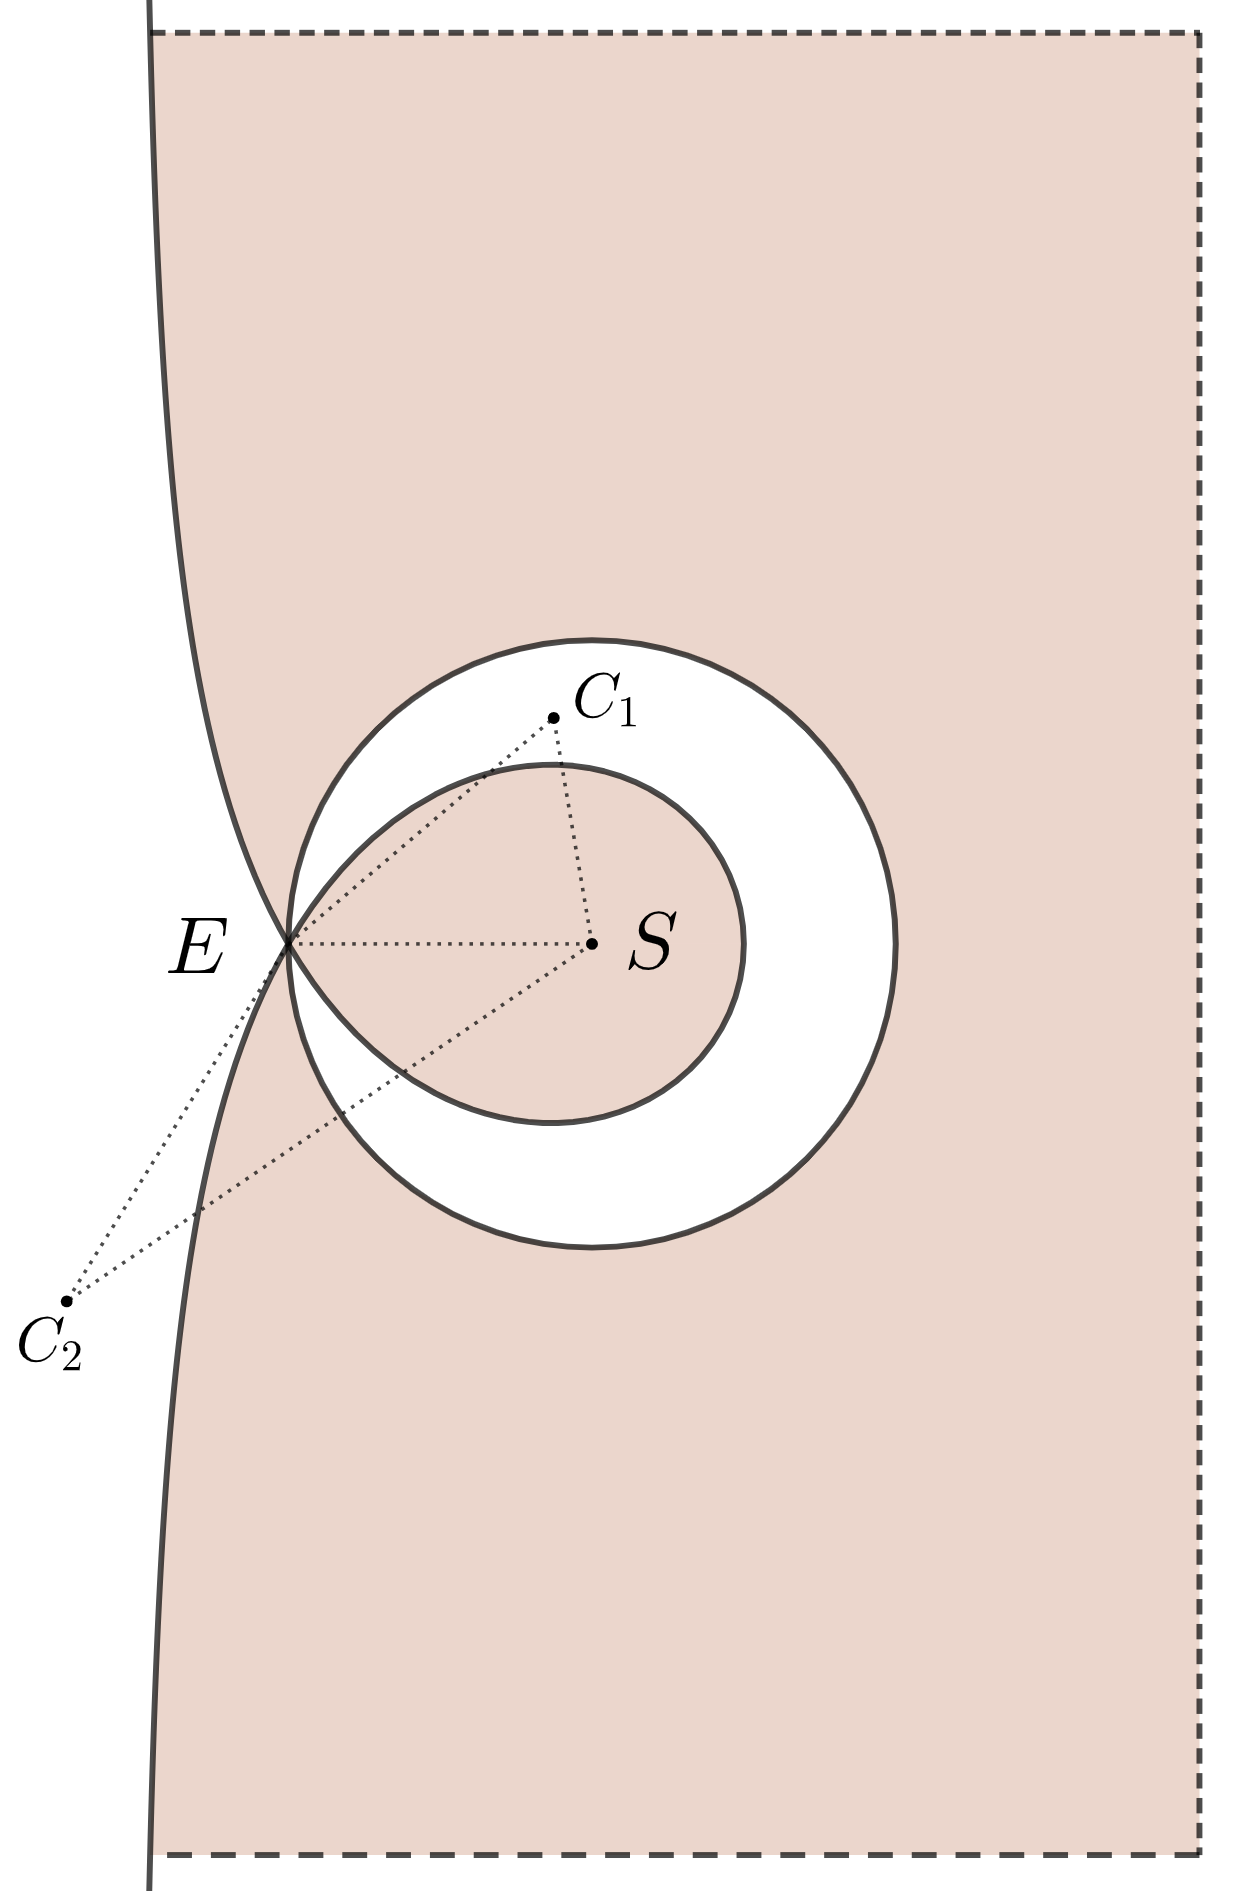
\includegraphics[scale=0.1]{images/seccion_superficie_unicidad.png}
	\hspace{1cm}
	\rulesep
	\hspace{1cm}
	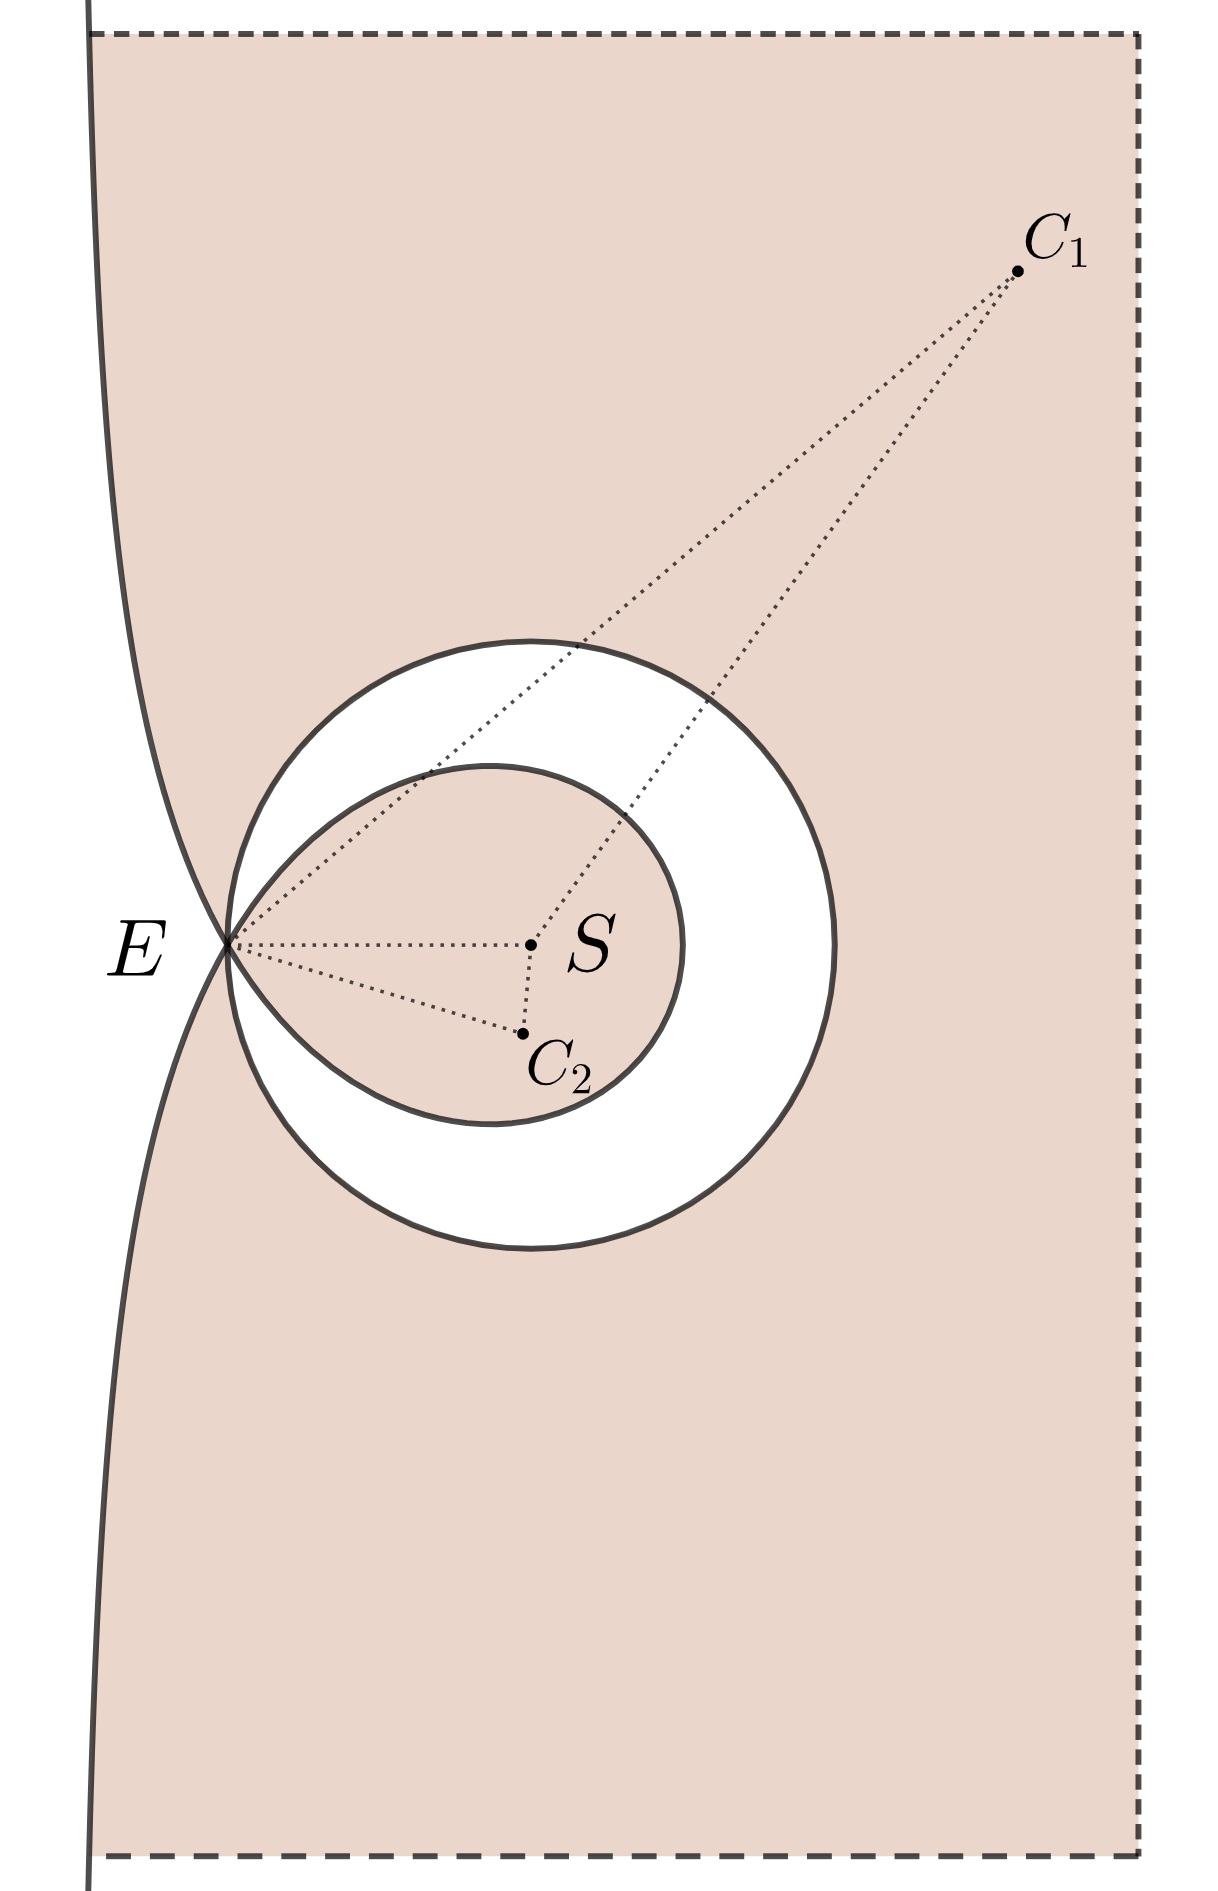
\includegraphics[scale=0.1]{images/seccion_superficie_no_unicidad.png}
}
\caption{Sección de la superficie de revolución junto a los casos en los que se da la unicidad y los que no. La región rosa se sigue extendiendo hasta el infinito.}
\label{fig:seccion_superficie}
\end{figure}

En la figura superior podemos ver que los límites para la condición de unicidad dividen el espacio en cuatro partes diferentes, dos sombreadas y las otras dos en blanco, de manera que las desigualdades de \eqref{eq:condicion_unicidad} mantienen el signo dentro de cada una de estas regiones y cambian de signo al cruzar la frontera de alguna de ellas.\\

Estudiemos ahora en cuál de estas regiones obtenemos una solución única y en cual doble. Para ello, tomemos un punto a la izquierda de $E$ en la recta $SE$, en el cuál se cumplirá que $r=\rho+R$ y $\psi=\pi$. Con esto, comprobemos la unicidad con \eqref{eq:condicion_unicidad}:
\[
\def\arraystretch{2}
\begin{array}{ll}
  & 1+\ddfrac{3D_1}{DR^4}\cos{\psi} = 1-\ddfrac{3D_1}{DR^4} = 1-\ddfrac{3}{R^4}\ddfrac{\rho}{\left(\ddfrac{1}{R^3}-\ddfrac{1}{r^3}\right)} = \\
= & 1-\ddfrac{3\rho}{R-\ddfrac{R^4}{r^3}} = 1-\ddfrac{3\rho}{R-\ddfrac{R^4}{(\rho+R)^3}} = 1-\ddfrac{3\rho}{\ddfrac{R(\rho+R)^3-R^4}{(\rho+R)^3}} = \\
= & 1-\ddfrac{3\rho(\rho+R)^3}{\rho^3R+3\rho^2R^2+3\rho R^3+R^4-R^4} = 1-\ddfrac{3(\rho+R)^3}{R(\rho^2+3\rho R+3R^2)}
\end{array}
\]

Podemos ver fácilmente que esta última igualdad es negativa para un valor grande de $\rho$, y ya que hemos supuesto previamente que $r>R$, se sigue que $\ddfrac{D_1}{D}>0$ y $N<0$, por lo que estamos en la primera desigualdad de \eqref{eq:condicion_unicidad}. Ya que esta desigualdad está satisfecha, podemos concluir que la solución del problema será única si el objeto observado se encuentra en el área no sombreada a la izquierda de $E$.\\

Cuando el objeto cruce de la región no sombreada a la izquierda de \ref{fig:seccion_superficie} a una región sombreada, manteniendo que $r>R$, la función cambiará de signo mientras que el signo de $N$ no cambie, en cuyo caso la primera desigualdad de \eqref{eq:condicion_unicidad} no se cumplirá y estaremos en el caso de una solución doble. En esta región, la primera función de \eqref{eq:condicion_unicidad} es positiva y $N$ es negativo, por lo que si cruzamos al área pequeña sin sombra la función pasa a ser negativa y $N$ positivo, satisfaciendo así la segunda desigualdad y deduciendo así que la solución es única. De manera similar, podremos comprobar que la solución es doble en la región sombreada pequeña.\\

Por tanto, el problema físico tiene solución única en los casos que vemos en la primera imagen de \ref{fig:seccion_superficie}, es decir, en las regiones blancas, y solución doble en los casos de la segunda imagen, las regiones sombreadas. \cite{moulton}\\



\section{Límites en $m$ y $M$.}
\label{sec:limites_m_M}
A la hora de determinar una órbita en un problema real, hemos de tener en cuenta que los valores $m$ y $M$ han de cumplir que las soluciones reales de la ecuación \eqref{eq:phi_solution} estén entre $0$ y $\pi$, pues sino el Sol, la Tierra y el objeto observado no formarían un triángulo. Por tanto, hemos de determinar los límites para que esta condición se satisfaga, y dichos límites pueden ser determinados mediante las condiciones para que obtengamos raíces dobles.\\

Para empezar, supongamos que $M$ es un valor fijo mientras $m$ varía. En el primer caso, que podemos ver en \ref{fig:phi_solution_m_negative_M_near_1}, se observan tres intersecciones de las curvas. Mientras $m$ vaya disminuyendo, la curva $y_2$ irá desplazándose hacia la derecha hasta que $\phi_1$ y $\phi_2$ pasen a ser iguales, teniendo así una raíz doble. De la misma manera, en \ref{fig:phi_solution_m_positive_M_near_1} observamos tres soluciones y, conforme $m$ aumente y desplace $y_2$ a la izquierda, $\phi_2$ y $\phi_3$ se igualarán.\\

\begin{figure}[H]
\centering
%\subfloat{
%	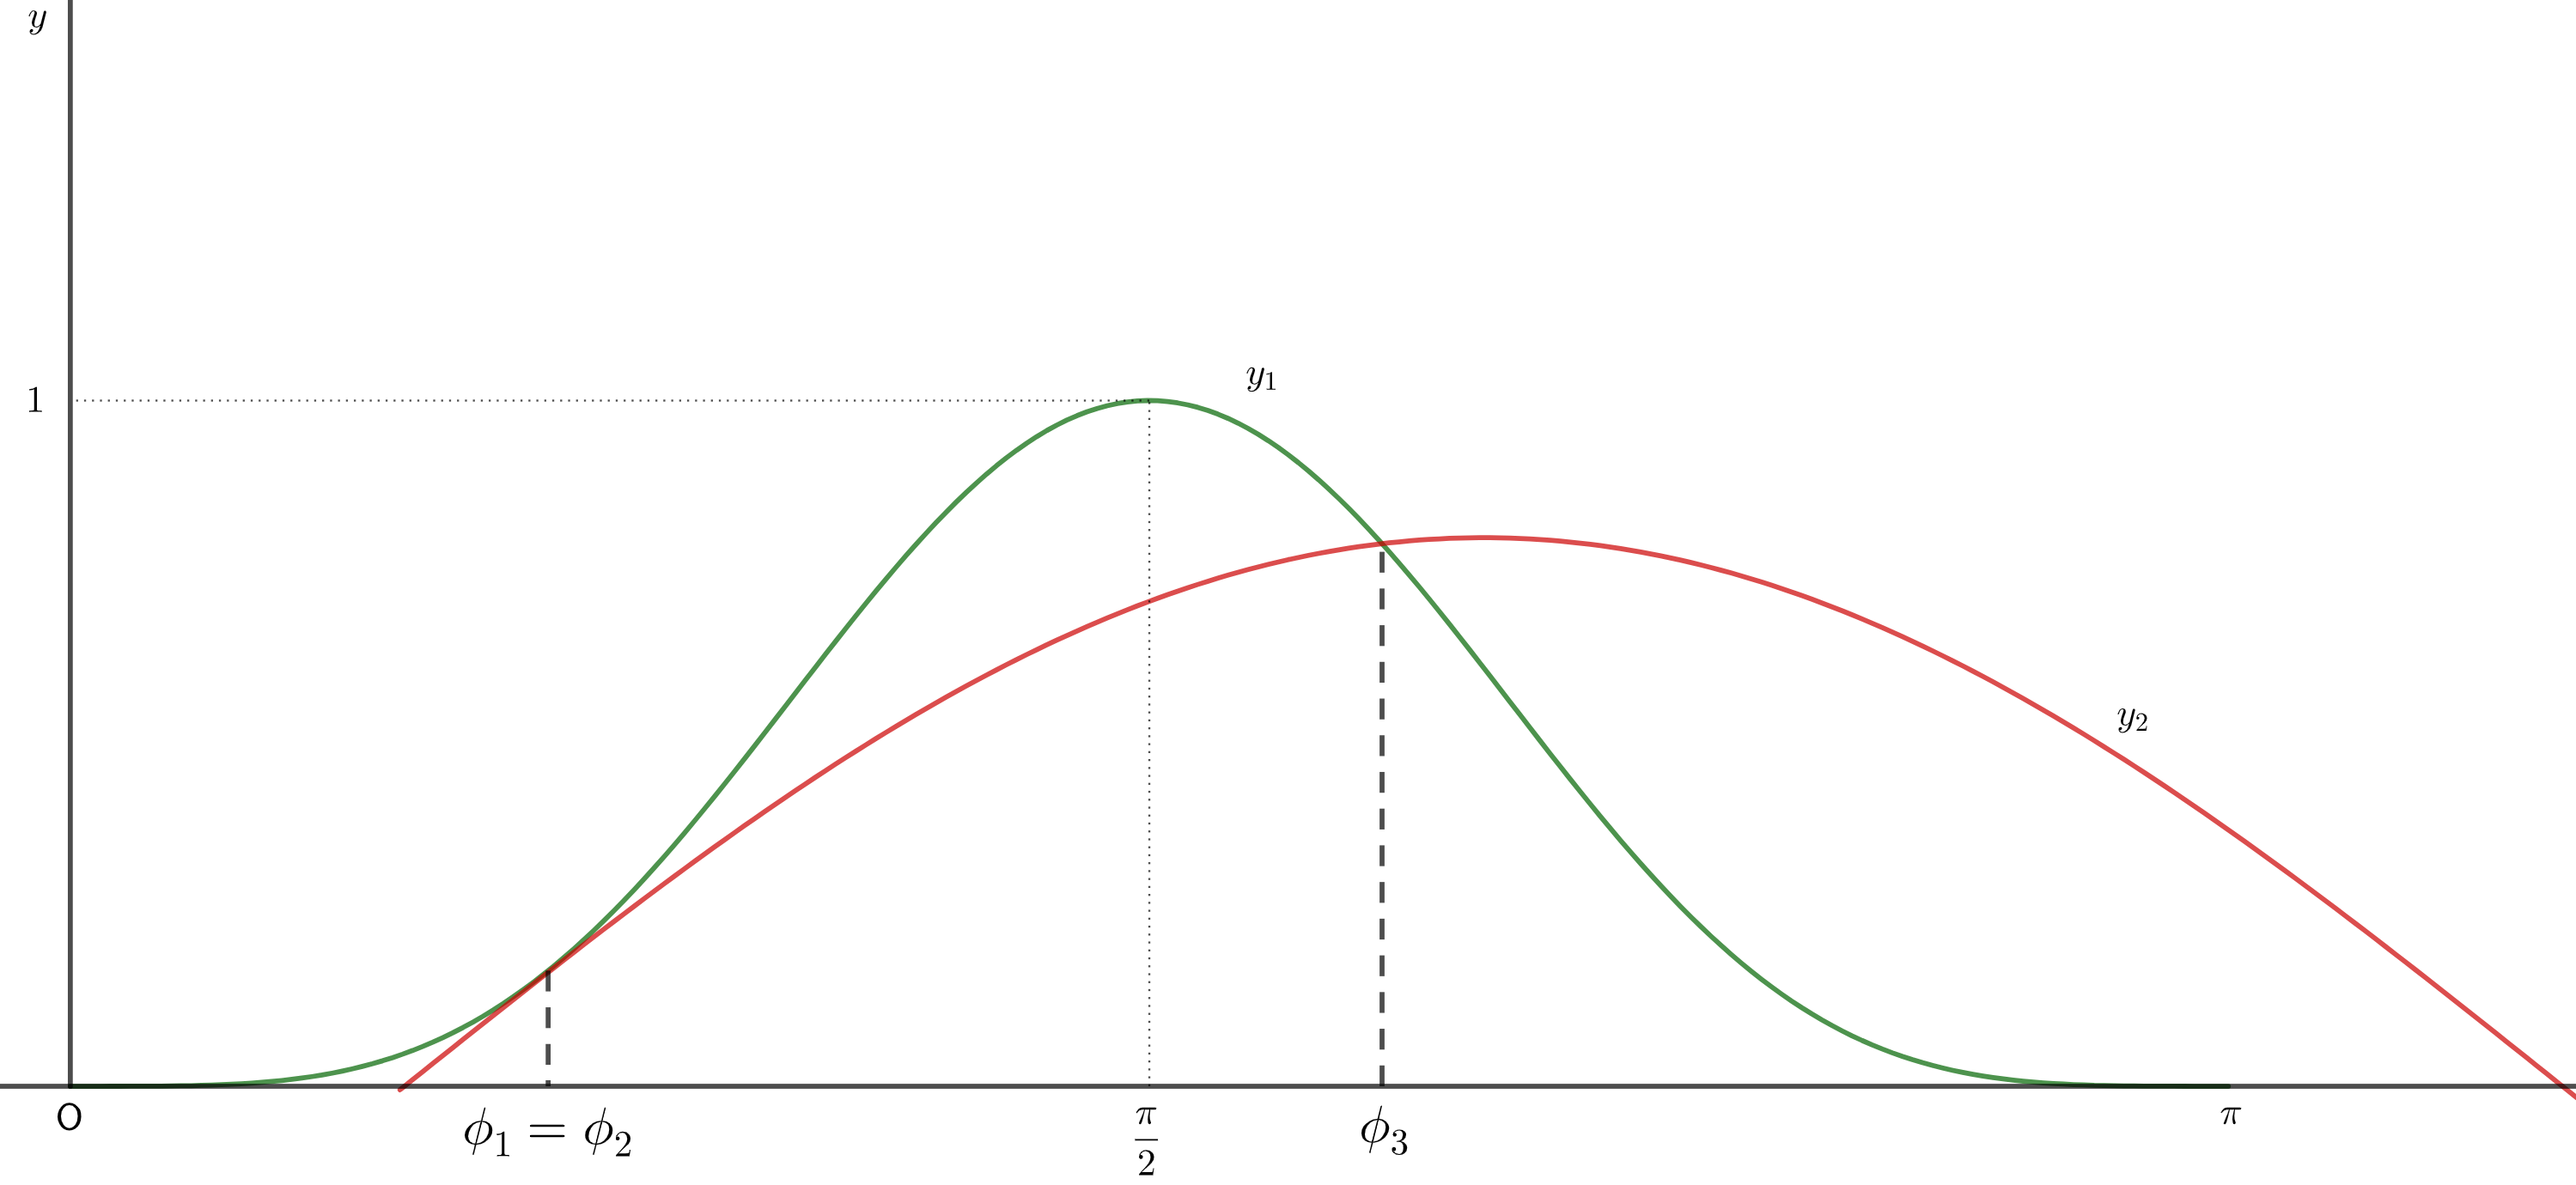
\includegraphics[scale=0.1]{images/minuscula_varia_primer_caso.png}
%	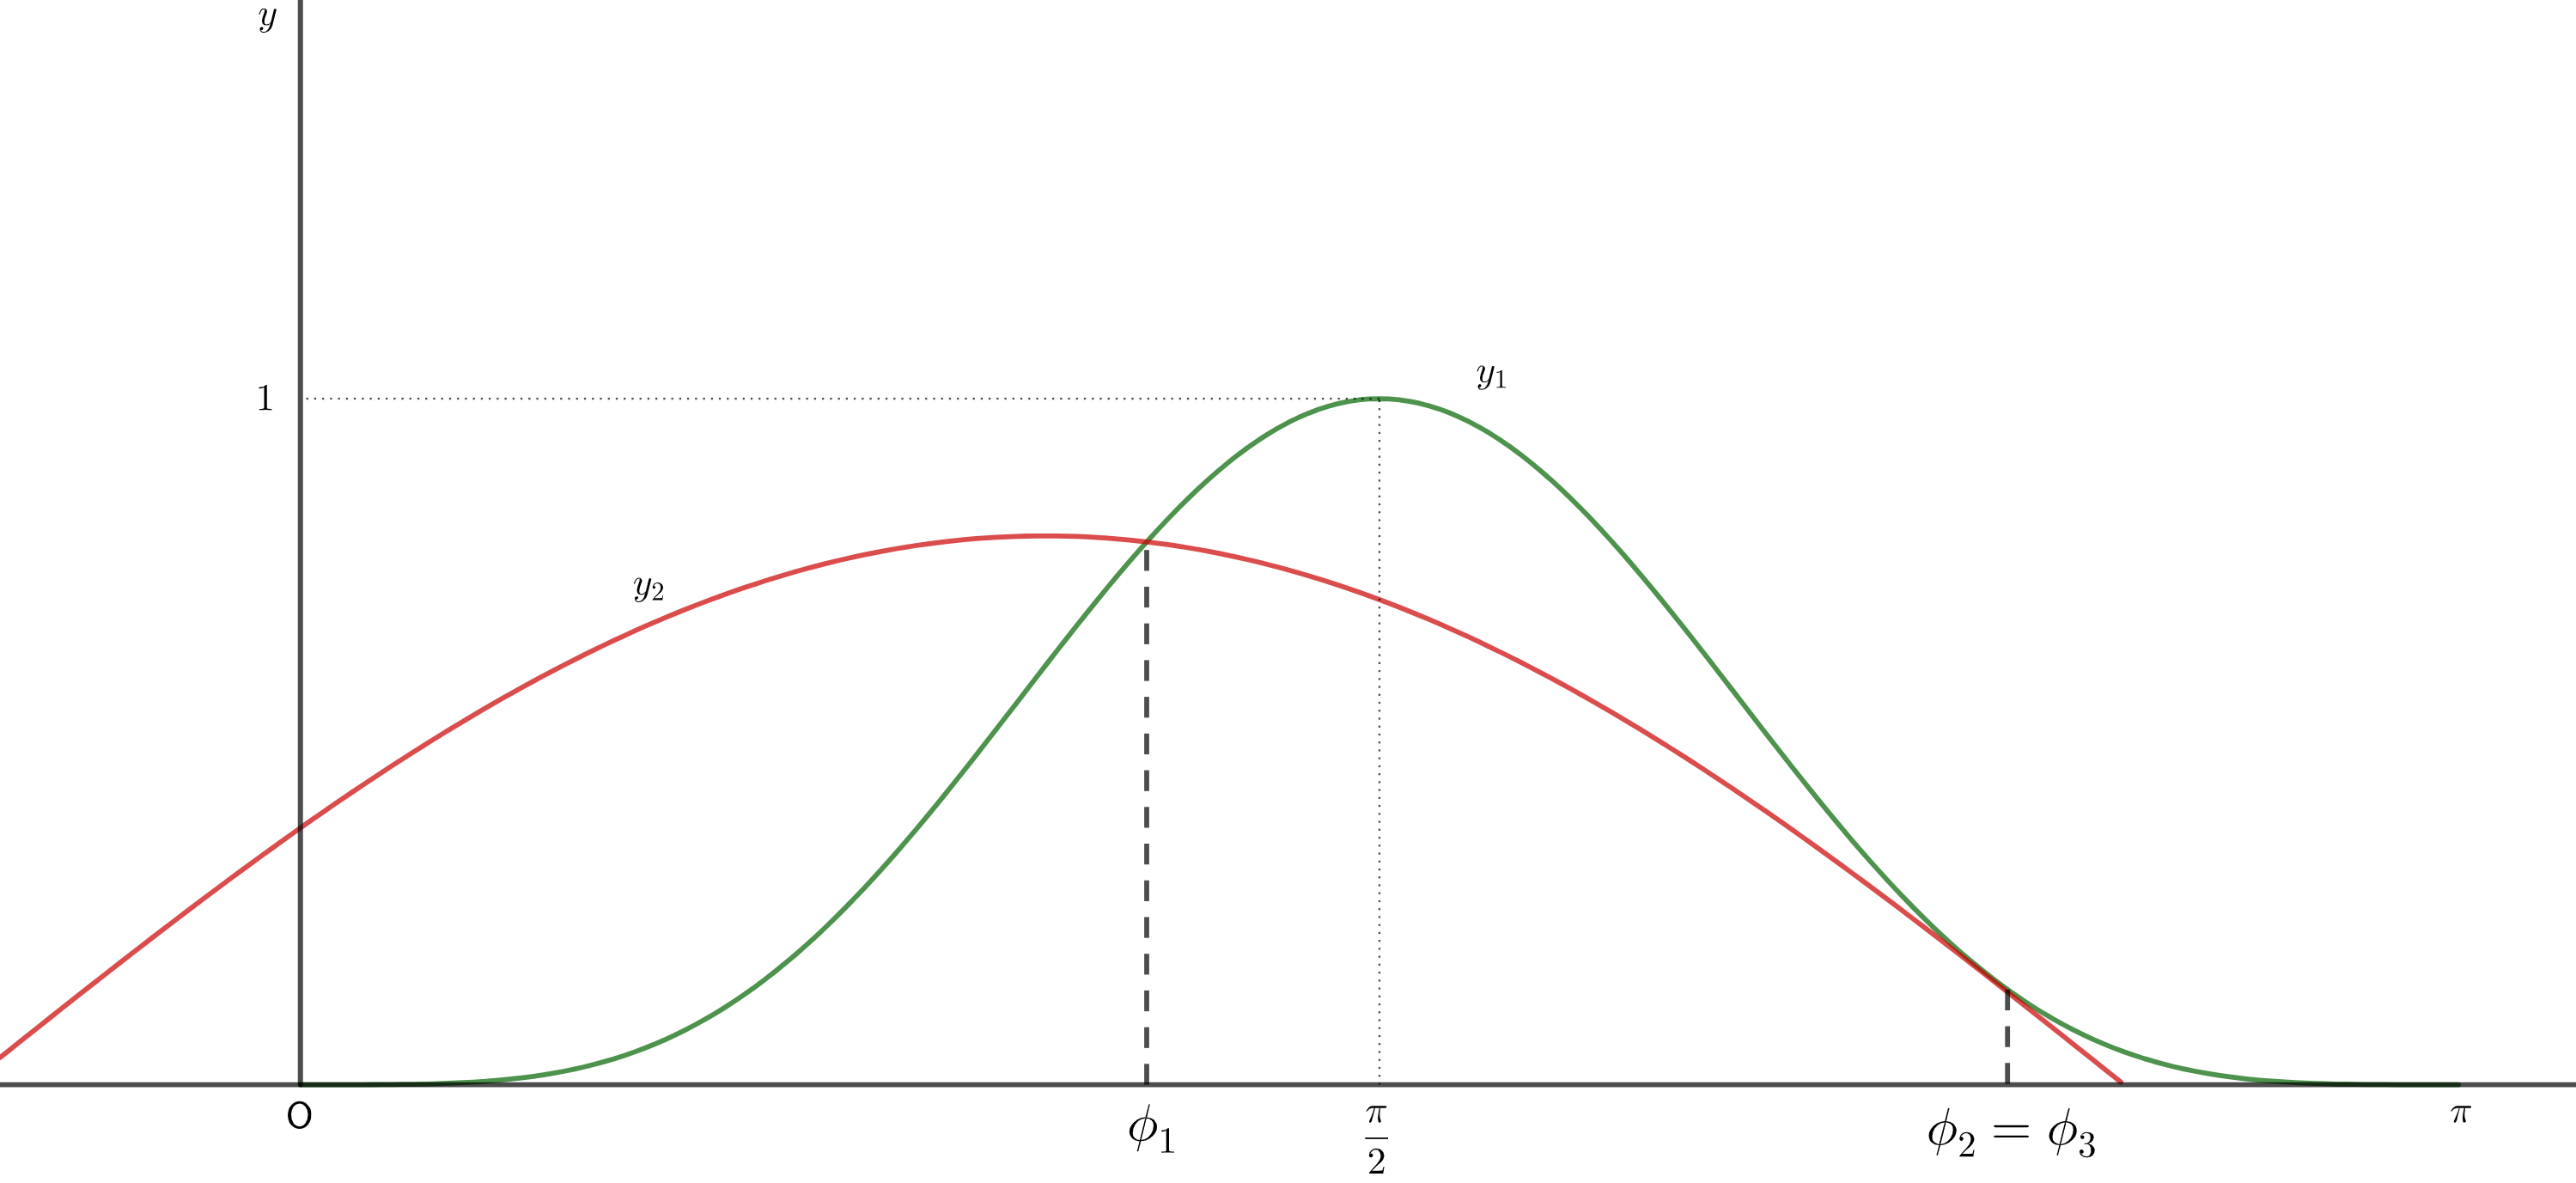
\includegraphics[scale=0.1]{images/minuscula_varia_segundo_caso.png}
%}
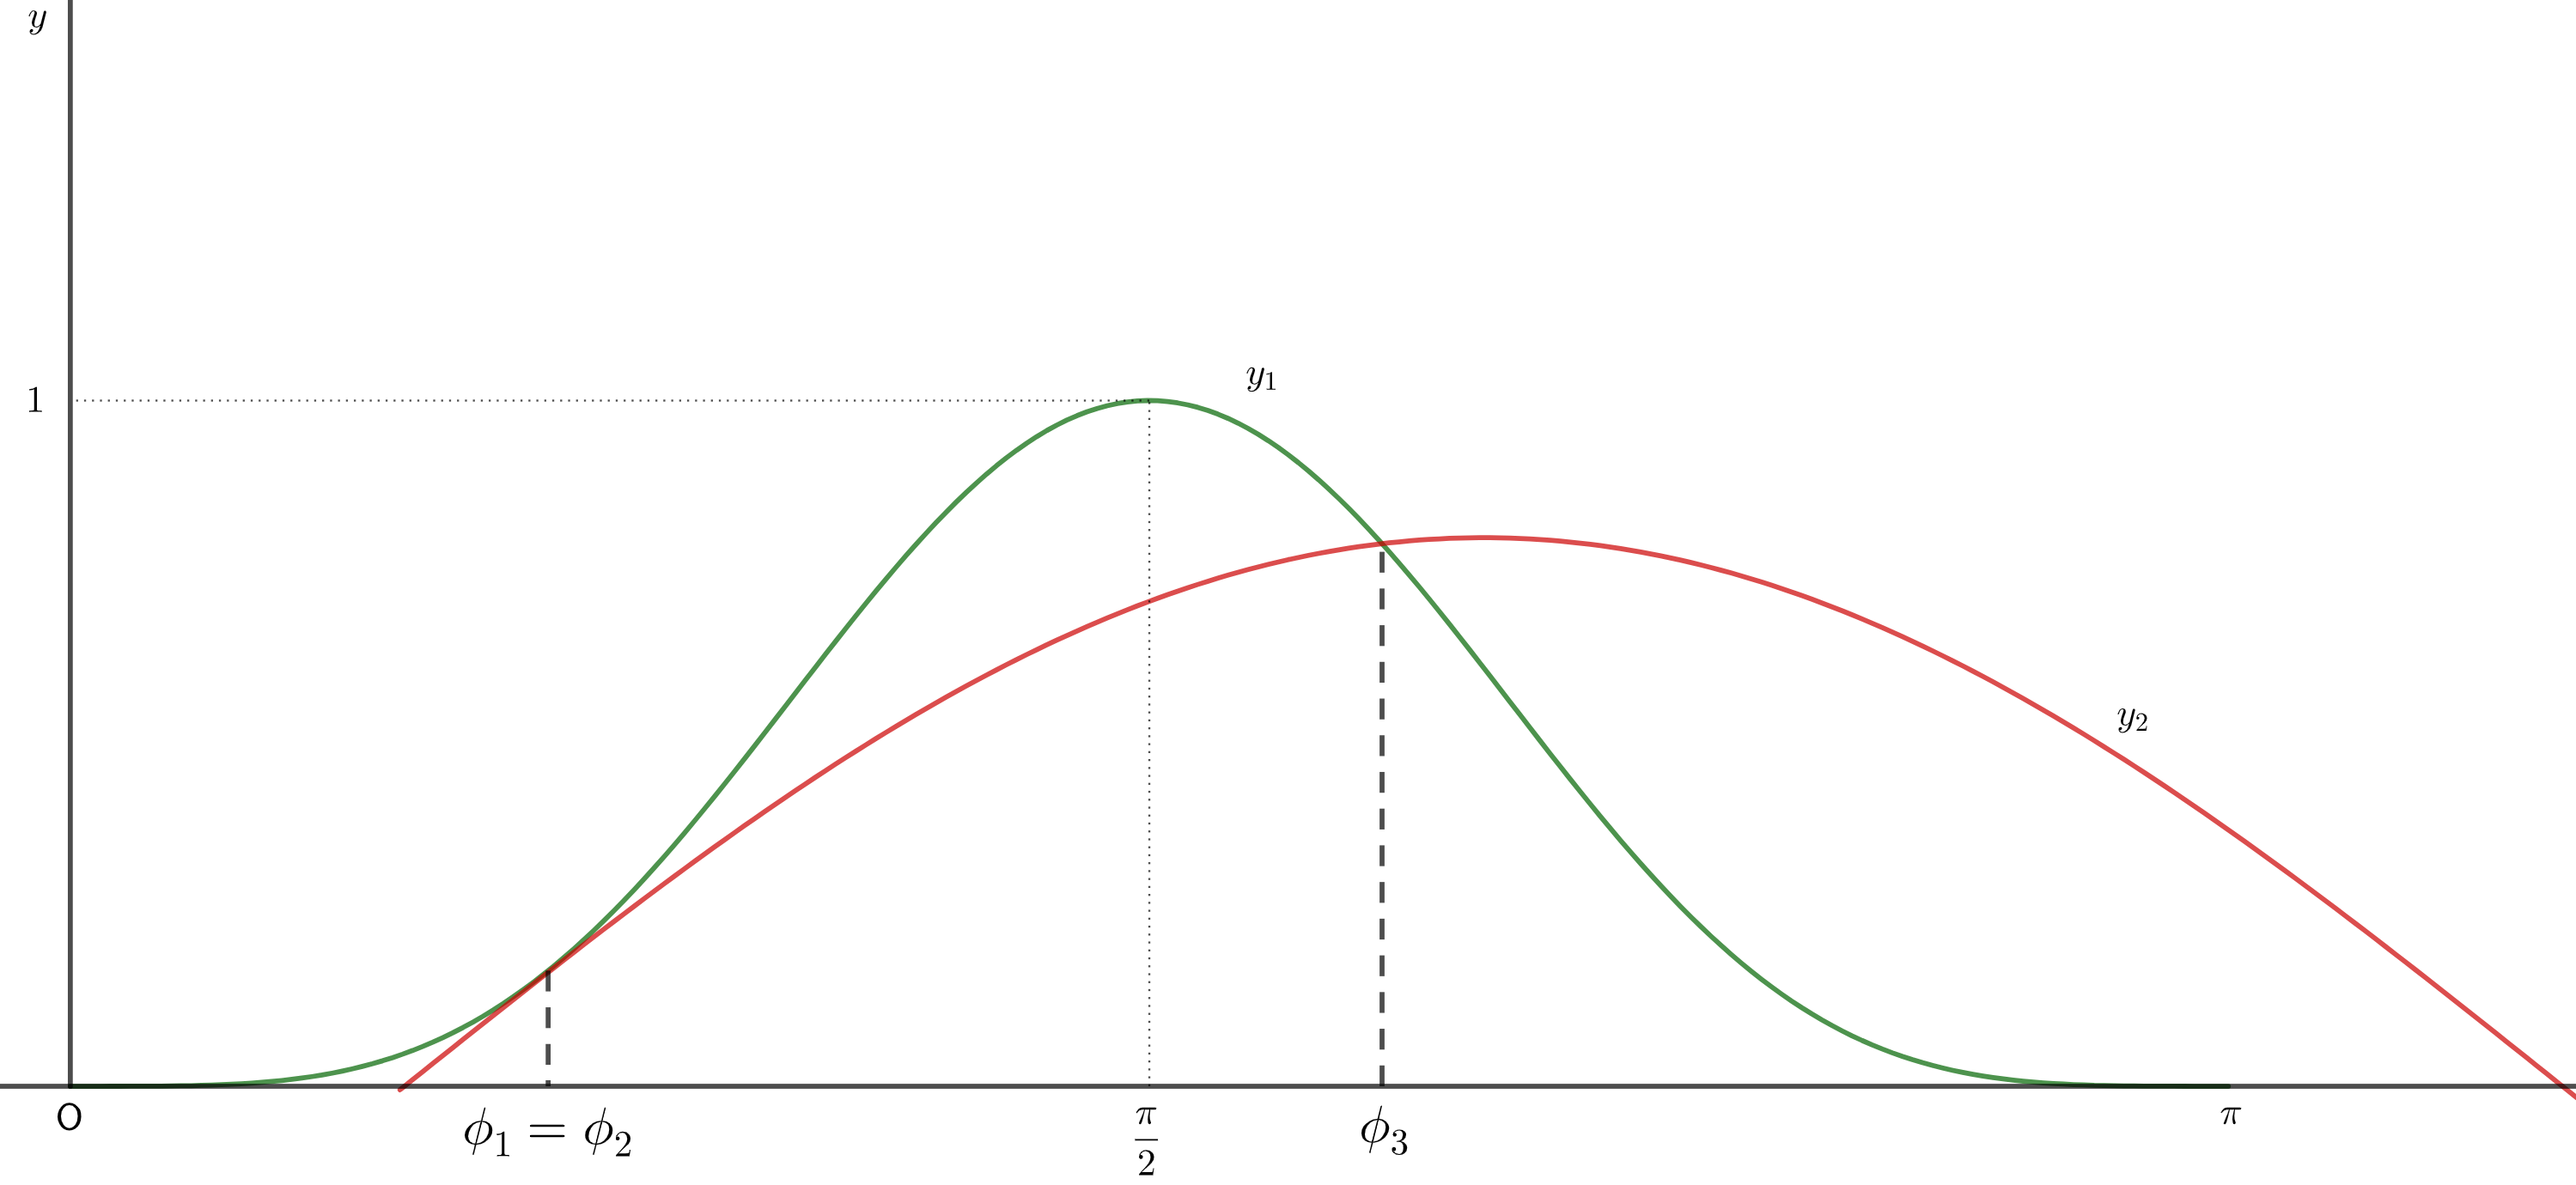
\includegraphics[scale=0.115]{images/minuscula_varia_primer_caso.png}
\caption{Variación de $m$ en la figura \ref{fig:phi_solution_m_negative_M_near_1} hasta obtener una solución doble.}
\label{fig:minuscula_varia_primer_caso}
\end{figure}

\begin{figure}[H]
\centering
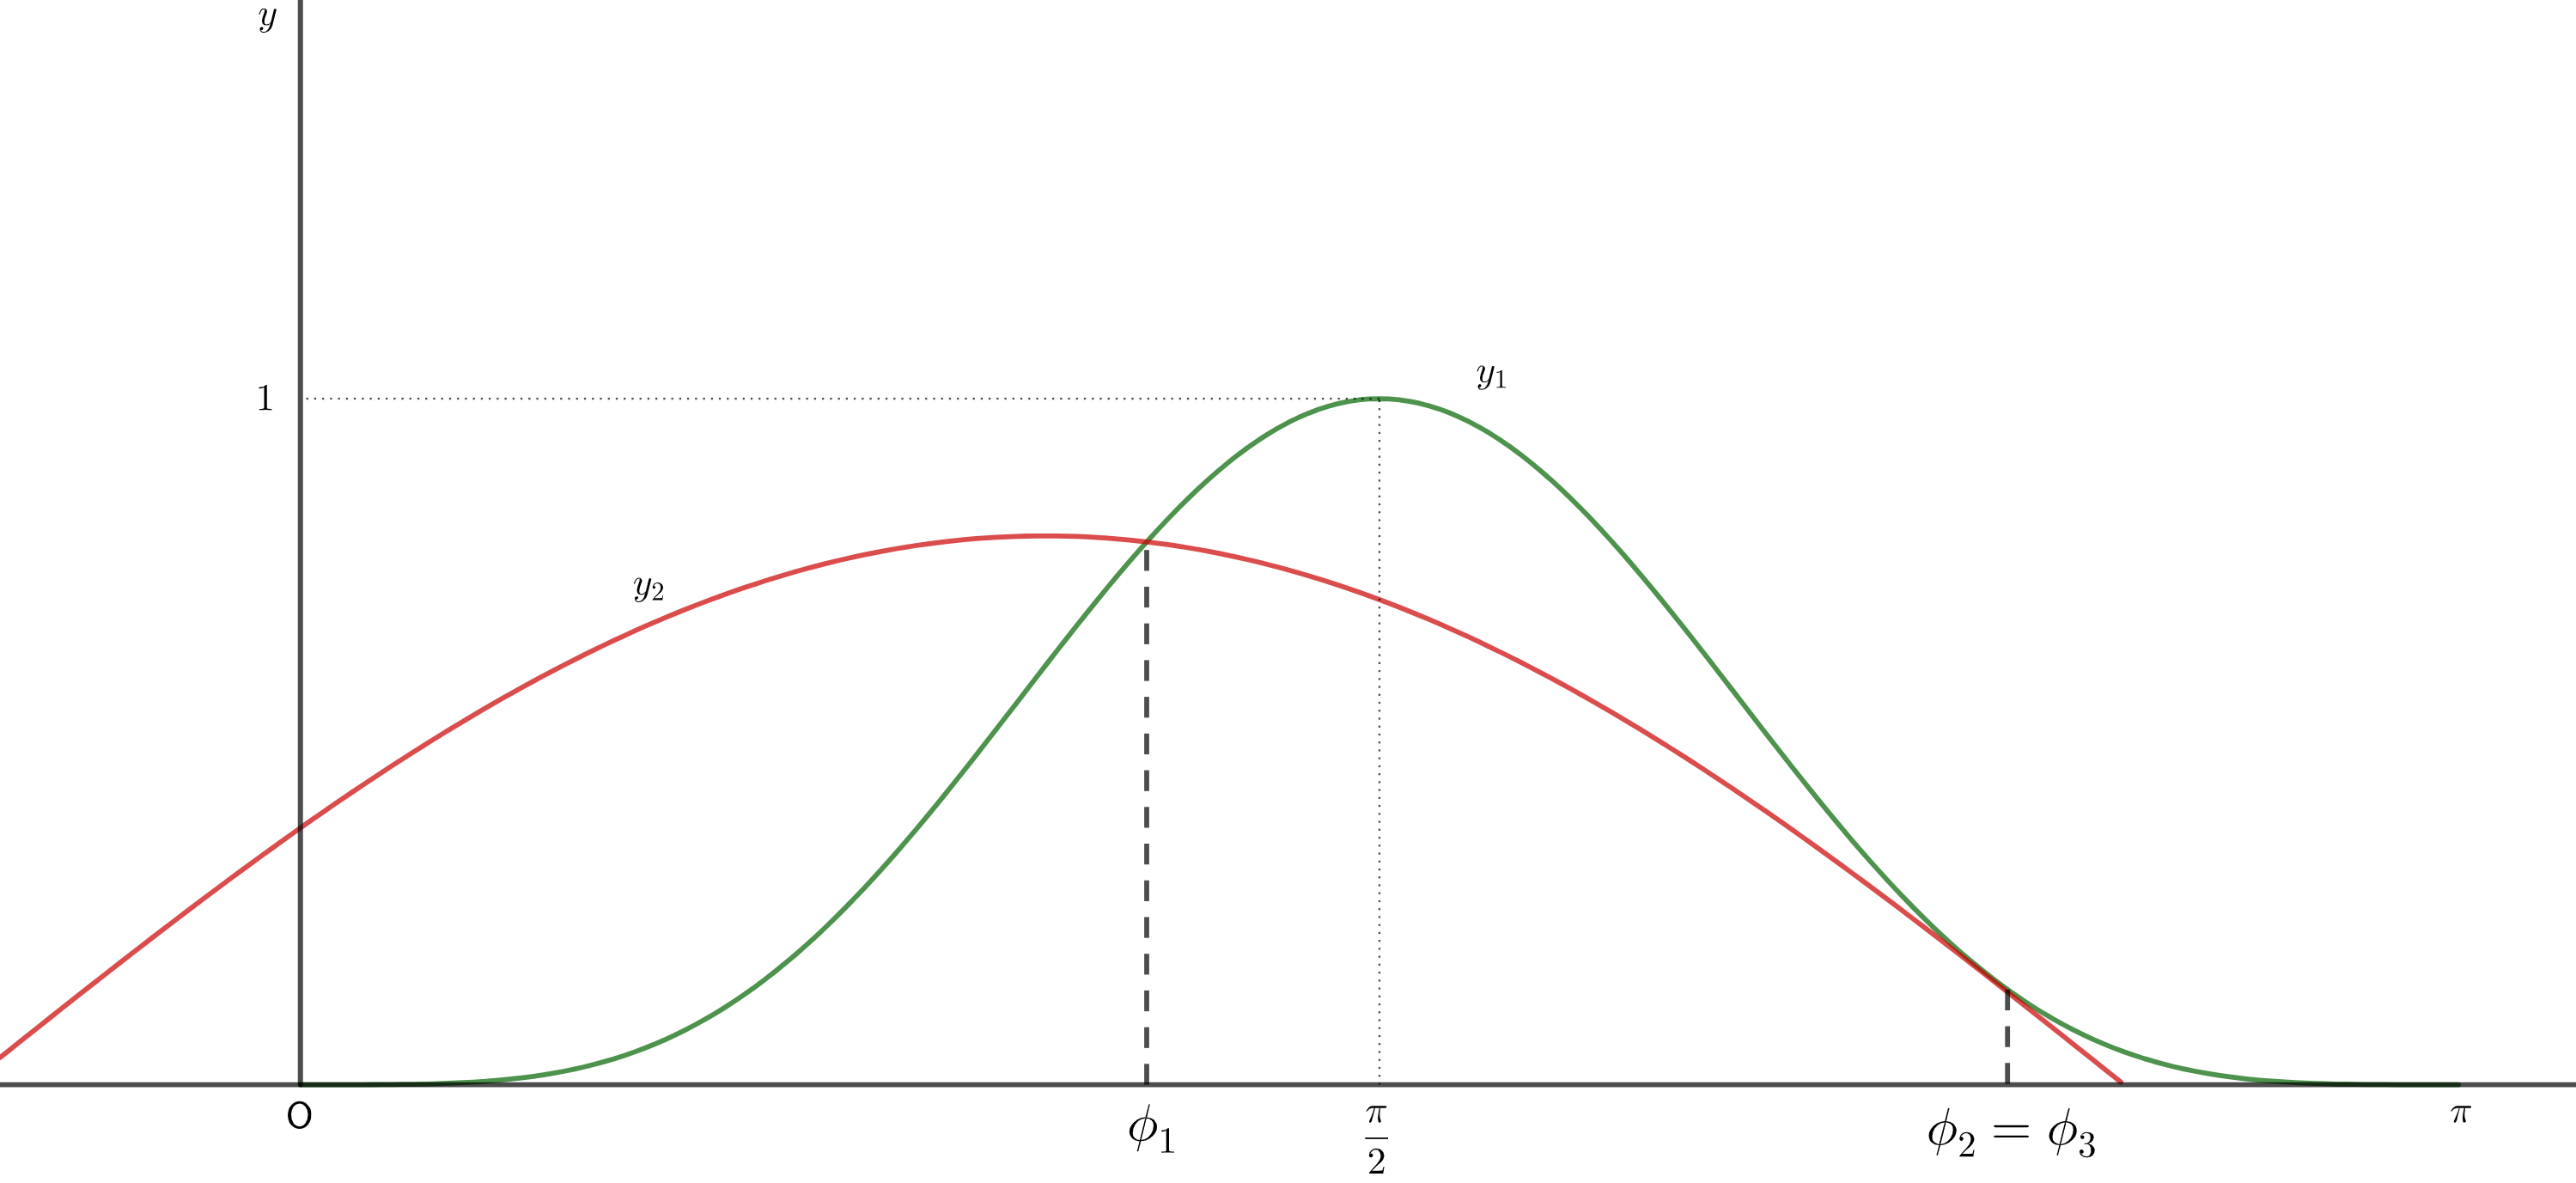
\includegraphics[scale=0.115]{images/minuscula_varia_segundo_caso.png}
\caption{Variación de $m$ en la figura \ref{fig:phi_solution_m_positive_M_near_1} hasta obtener una solución doble.}
\label{fig:minuscula_varia_segundo_caso}
\end{figure}

Veamos ahora el otro caso; fijamos $m$ y vamos aumentando $M$ empezando desde un valor pequeño. Conforme $M$ aumente, la amplitud de $y_2$ aumentará, dejando fijo, en el primer caso (figura \ref{fig:phi_solution_m_negative_M_near_1}), $\phi_1$ y llegando a un punto donde $\phi_2$ y $\phi_3$ serán iguales. Funcionará análogamente con el segundo caso.

\begin{figure}[H]
\centering
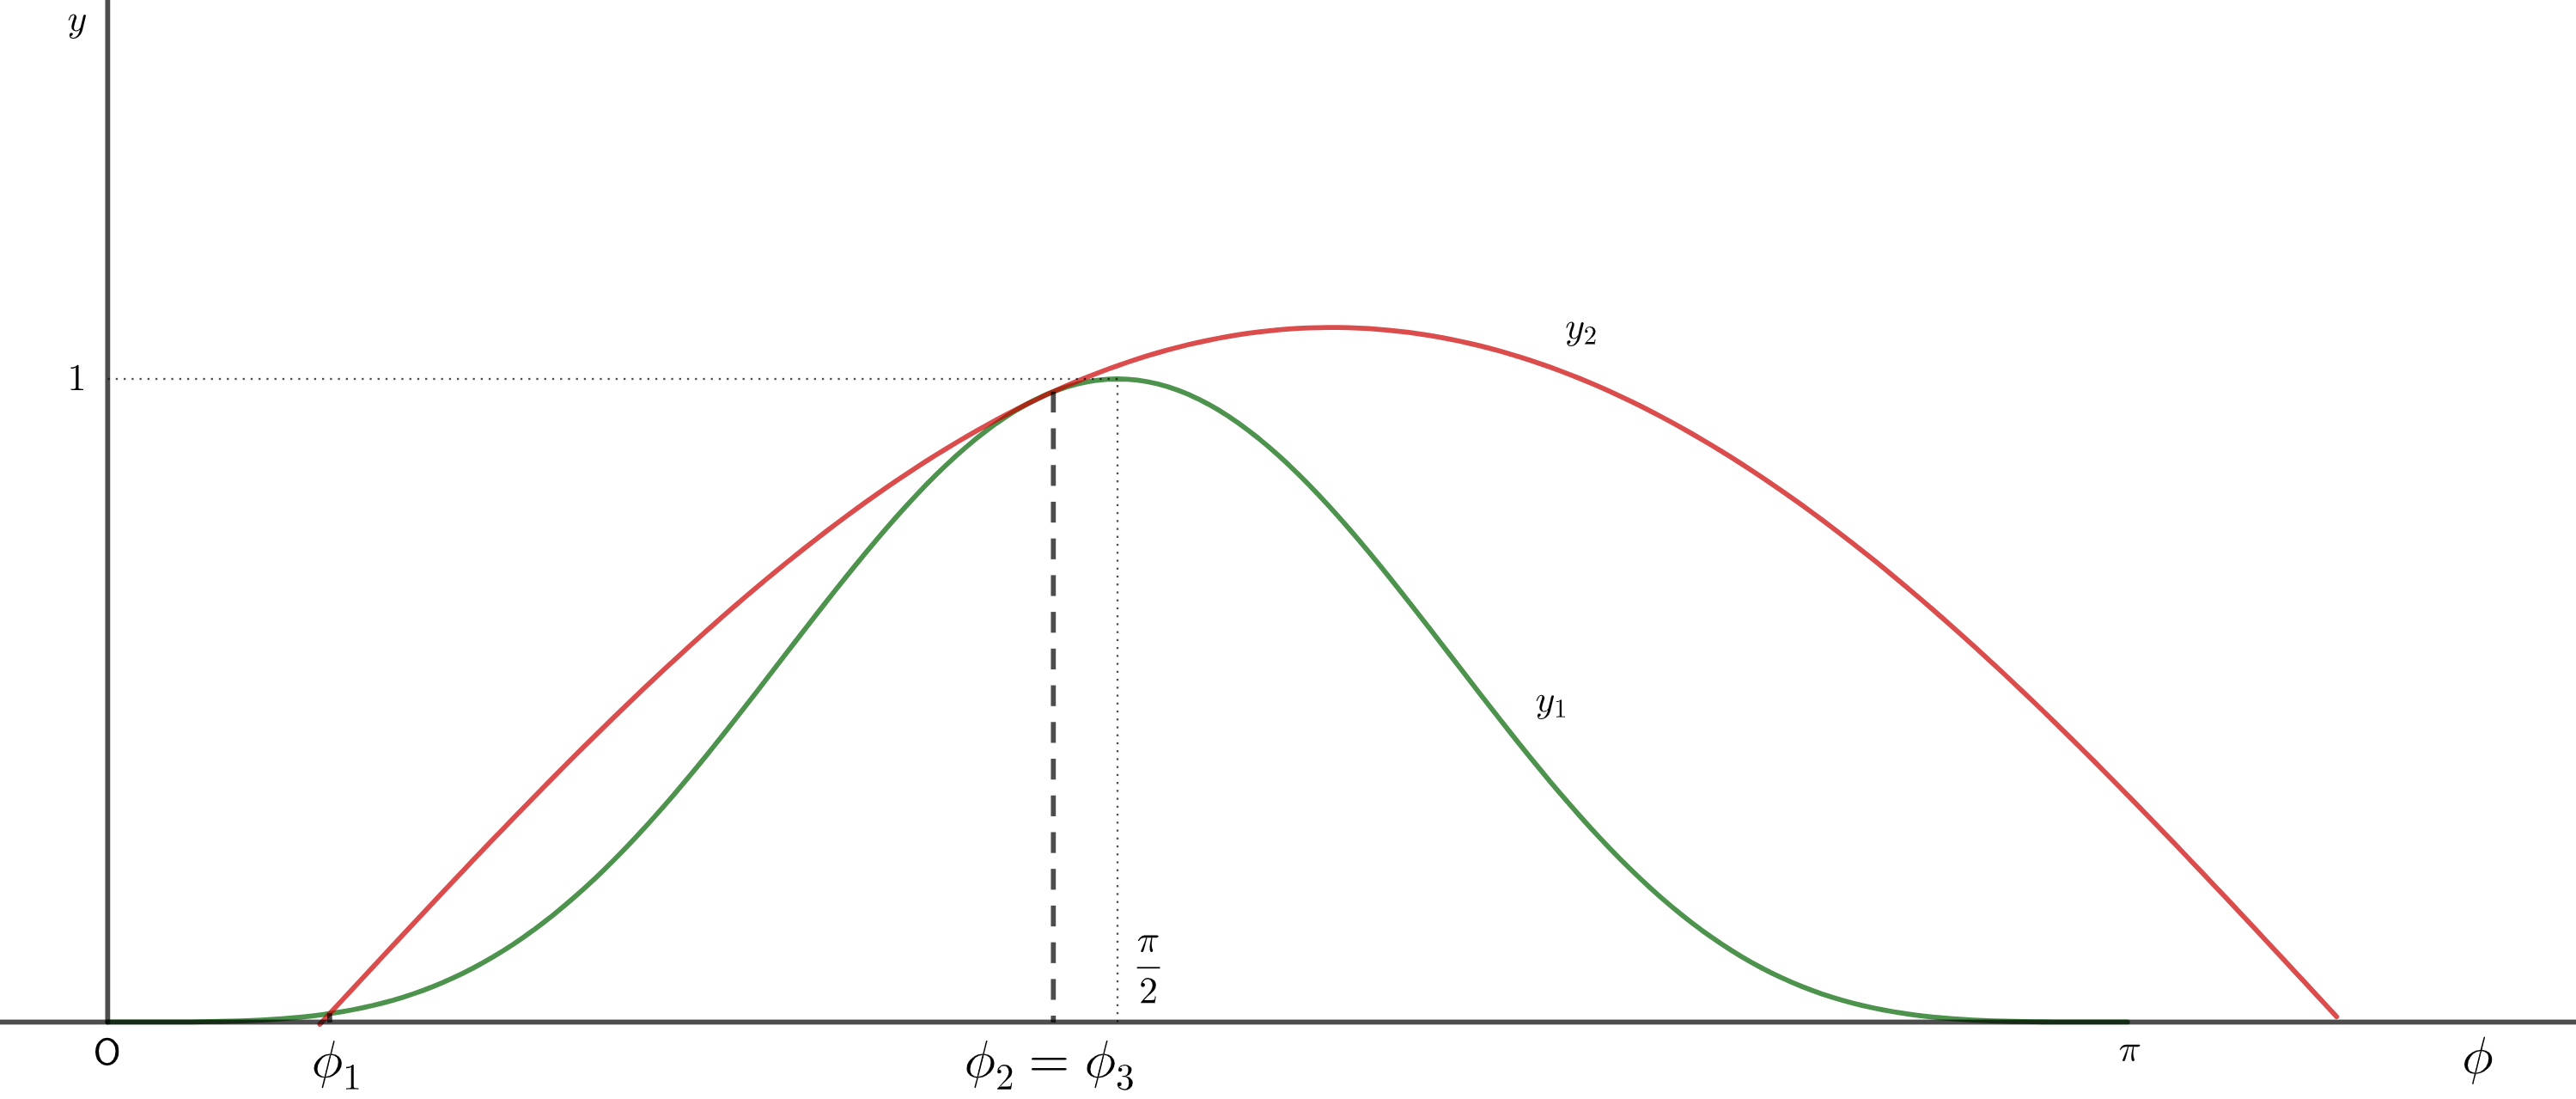
\includegraphics[scale=0.115]{images/mayuscula_varia_primer_caso.png}
\caption{Variación de $M$ en la figura \ref{fig:phi_solution_m_negative_M_near_1} hasta obtener una solución doble.}
\label{fig:mayuscula_varia_primer_caso}
\end{figure}

\begin{figure}[H]
\centering
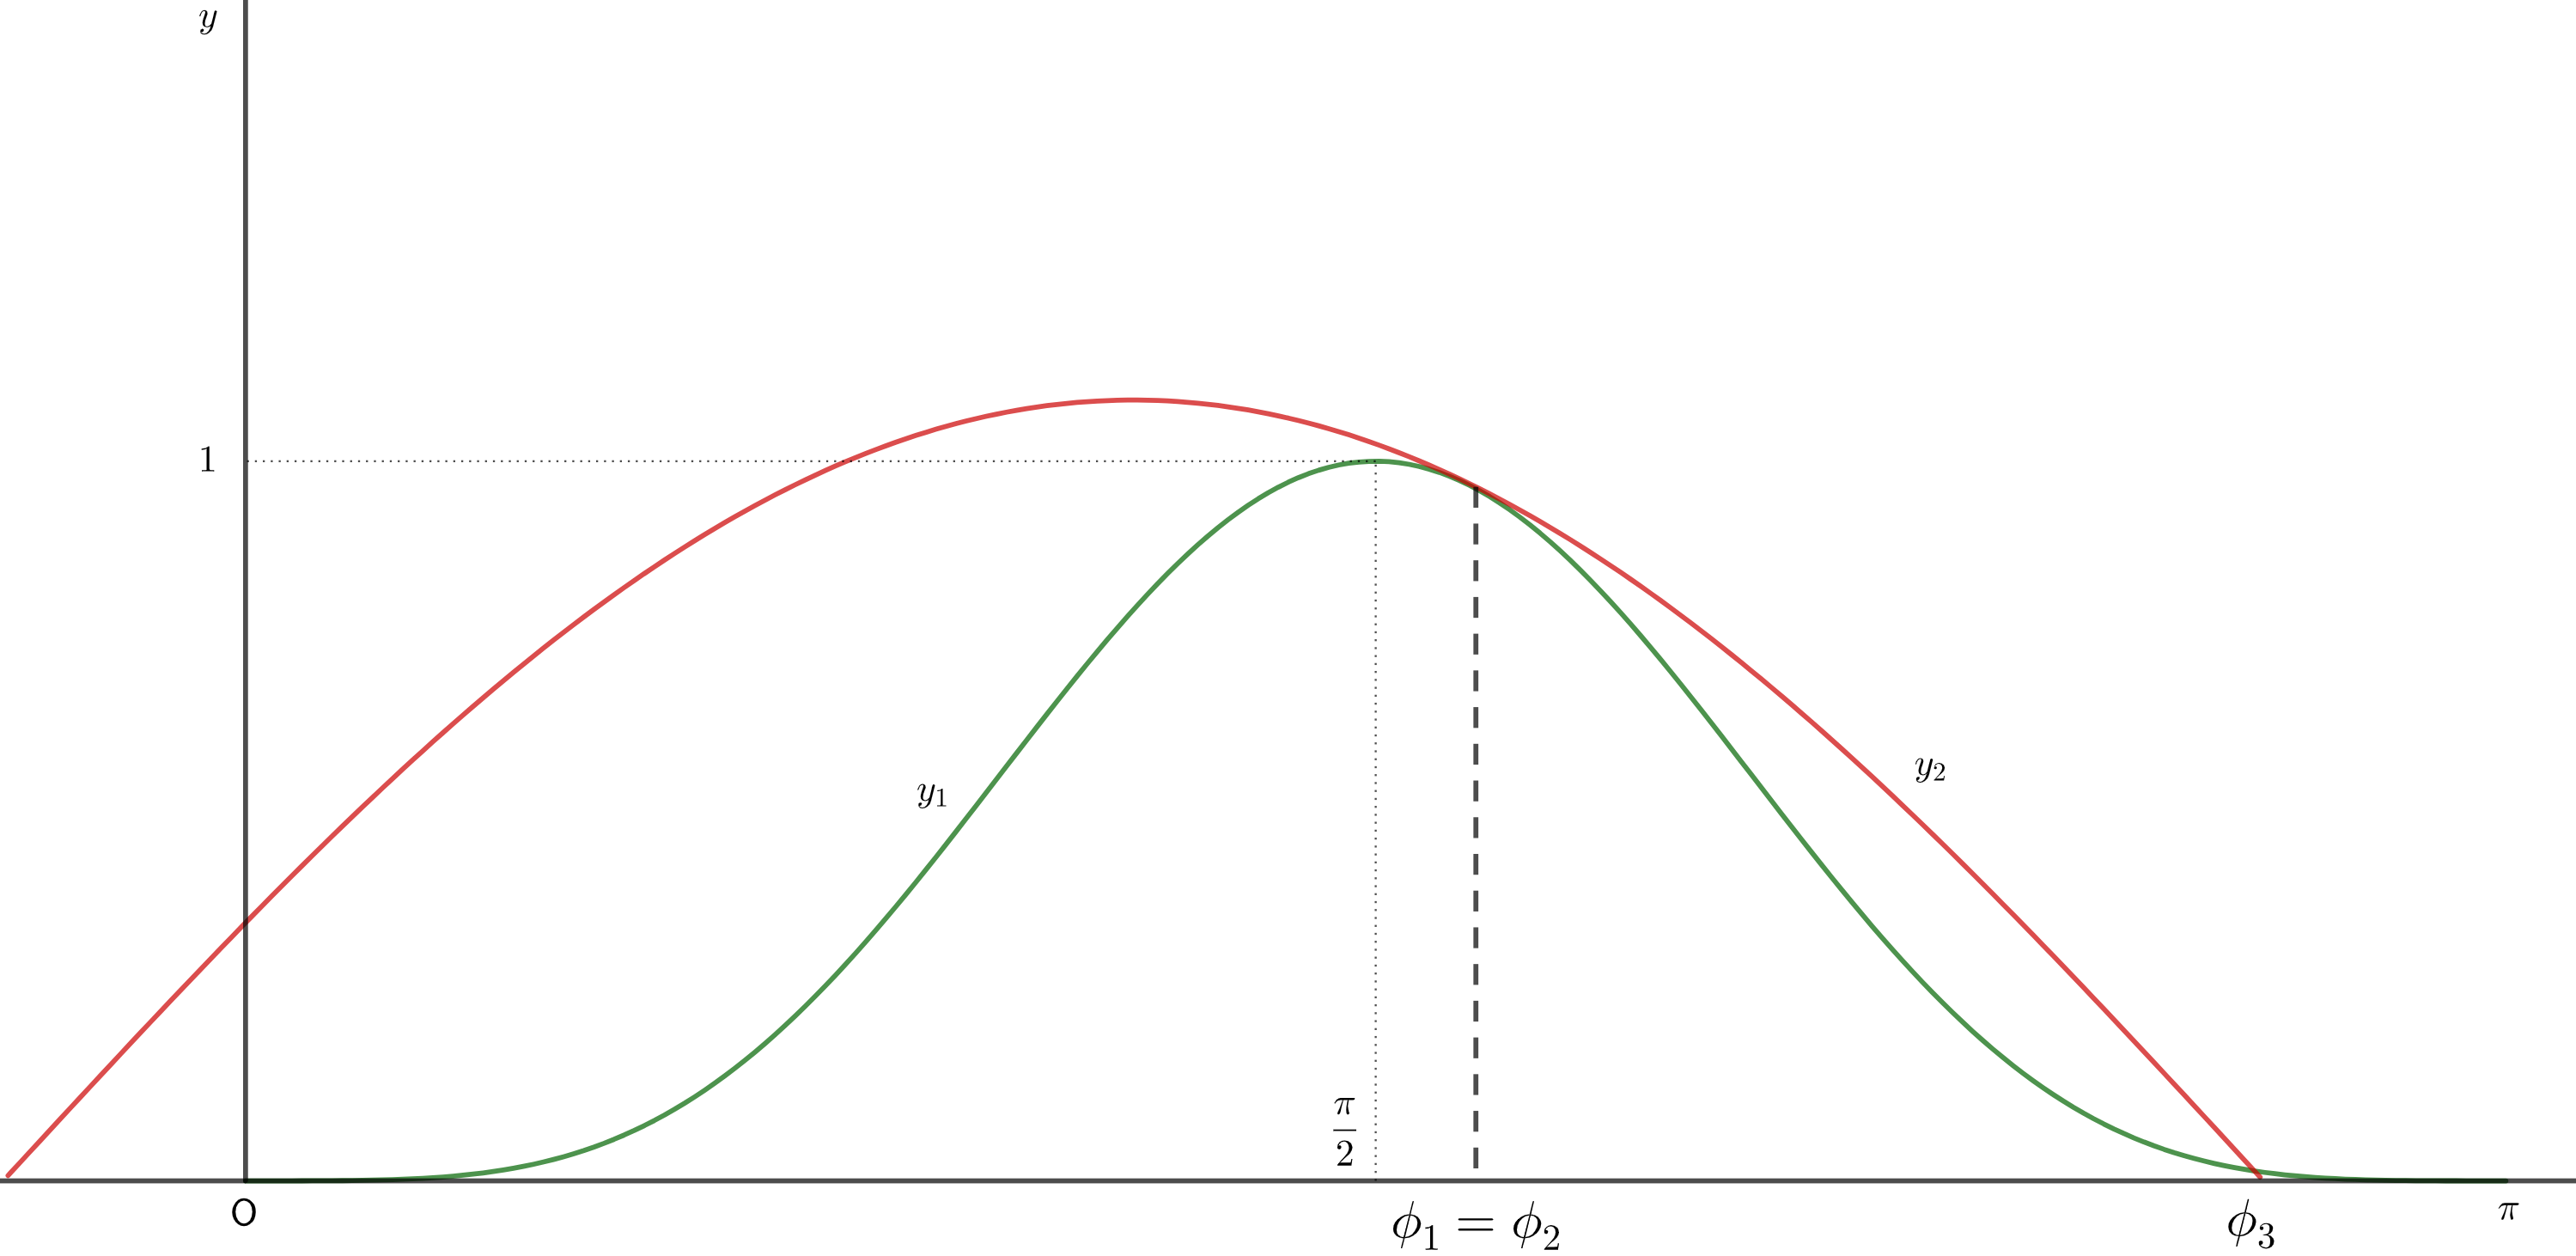
\includegraphics[scale=0.115]{images/mayuscula_varia_segundo_caso.png}
\caption{Variación de $M$ en la figura \ref{fig:phi_solution_m_positive_M_near_1} hasta obtener una solución doble.}
\label{fig:mayuscula_varia_segundo_caso}
\end{figure}

Las condiciones en las que la ecuación \eqref{eq:phi_solution} tendrá una solución doble son:
\begin{align}
\left\{
\begin{array}{l}
	\sin^4{\phi}=M\sin{(\phi+m)}\\
	4\sin^3{\phi}\cos{\phi}=M\cos{(\phi+m)}
\end{array}
\right.
\label{eq:condicion_raiz_doble}
\end{align}

Con el fin de encontrar las condiciones a las que esté sujeto $m$ para que la raíz sea doble, dividamos las dos ecuaciones superiores y resolvamos para la $\tan{\phi}$.
\begin{align}
\def\arraystretch{2}
\begin{array}{ll}
  & \ddfrac{\sin^4{\phi}}{4\sin^3{\phi}\cos{\phi}}=\ddfrac{M\sin{(\phi+m)}}{M\cos{(\phi+m)}}\Longrightarrow \ddfrac{1}{4}\tan{\phi}=\tan{(\phi+m)}\\
\Longrightarrow & \ddfrac{1}{4}\tan{\phi}=\ddfrac{\tan{m}+\tan{\phi}}{1-\tan{m}\tan{\phi}} \Longrightarrow \tan{\phi}-(\tan{\phi})^2\tan{m}=4\tan{m}+4\tan{\phi}\\
\Longrightarrow & \tan^2{\phi}\tan{m}+3\tan{\phi}+4\tan{m}=0 \Longrightarrow \tan{\phi}=\ddfrac{-3\pm\sqrt{9-16\tan^2{m}}}{2\tan{m}}
\end{array}
\label{eq:tan_phi}
\end{align}

Así, para que $\tan{\phi}$ tenga soluciones reales $m$ ha de estar sujeto a la condición:
\[
9-\tan^2{m}\geq0,
\]
\noindent y resolviendo esta inecuación para $m$ obtendremos:
\begin{align}
\left\{
\begin{array}{l}
	0 \leq m \leq 36º52'\\
	323º8' \leq m \leq 360º
\end{array}
\right.
\label{eq:m_condition}
\end{align}

El primer rango de valores pertenecerá al segundo caso comentado, representado en la figura \ref{fig:phi_solution_m_positive_M_near_1}, y viceversa.\\

Utilizando este rango de valores, para cada $m$ habrá dos soluciones de \eqref{eq:tan_phi} en el intervalo $(0,\pi)$. Si tomamos $m$ entre $323º8'$ y $360º$, la tangente de $m$ será negativa y $\tan{\phi}$ será positiva independientemente de qué signo tomemos antes de la raíz; además, $\tan{\phi}$ será menor cuando cojamos el signo negativo. De tal manera, si tomamos el radical positivo estaremos en el caso $\phi_1=\phi_2$ (figura \ref{fig:minuscula_varia_primer_caso}) y si lo tomamos negativo estaremos en el caso $\phi_2=\phi_3$ (figura \ref{fig:mayuscula_varia_primer_caso}). Por último, si tomamos $m$ como un valor límite del intervalo estaremos ante el caso $9-\tan^2{m}=0$, por lo que $\phi_1=\phi_2=\phi_3$. Si tomamos el caso $0 \leq m \leq 36º52'$ tendremos que $\tan{m}>0$ y la discusión será análoga a la anterior.\\

Los valores límite de $\phi$ definidos por \eqref{eq:tan_phi} según el rango de valores para $m$ serán:
\begin{align}
\phi=\arctan{(\ddfrac{-3}{2\tan{m}})} \Longrightarrow
\left\{
\begin{array}{l}
	\phi=116º34'\\
	\phi=63º26'
\end{array}
\right.
\end{align}

Utilizando estos valores de $\phi$ podemos obtener un valor para $M$ mediante las ecuaciones \eqref{eq:condicion_raiz_doble}, $M=1.431$, y dicho valor se corresponderá con el máximo $M$ para el cuál \eqref{eq:phi_solution} tiene tres soluciones en el intervalo $(0,\pi)$.\\

Supongamos que $m$ toma el valor límite $323º8'$ y va aumentando hasta su límite superior, $360º$. Como hemos visto anteriormente, comenzaremos teniendo una raíz doble y los dos valores de $\phi$ se corresponderán con $63º26'$, y conforme $m$ aumente, una de las soluciones irá hacia $0º$ mientras la otra irá hacia $90º$. Respecto a como cambian las soluciones en función de $M$, comenzaremos en el límite, $M=1.431$, e iremos reduciendo su valor hasta cero. Si $m=36º52'$, conforme vaya decreciendo $M$ la solución irá hasta $0$, y si $m=323º8'$ nuestra solución crecerá hasta $\pi$. Notar que para cada $m$ que tomemos en los intervalos definidos en \eqref{eq:m_condition} existirán dos límites de $M$ de manera que \eqref{eq:phi_solution} tenga tres soluciones reales; por tanto, estos límites han de ser tenidos en cuenta con el fin de reducir el trabajo lo máximo posible. \cite{moulton}\\





\markedchapter{Implementación}{Implementación de un software para la aproximación de órbitas}
\label{chap:implementation}
Una vez hemos estudiado el método de Laplace para la determinación de órbitas mediante tres observaciones, nos centraremos en desarrollar un programa que sea capaz de realizar estos cálculos y mostrar los resultados de manera visual para hacer más fácil la aproximación. Además, éste nos servirá de ayuda para comprobar la precisión con la que se determina una órbita mediante el método laplaciano.\\

Antes de hablar sobre el programa y todas sus funcionalidades, centrémonos en las herramientas que se han utilizado para todo el desarrollo.\\

\section{Herramientas utilizadas.}
\label{sec:herramientas}
Tal y como comentamos en la introducción, todo el código implementado para el funcionamiento de nuestro software está en lenguaje Python. Uno de los motivos por los que se ha tomado la decisión de elegir este lenguaje de programación es el hecho de que durante la carrera nos hemos familiarizado con él dado que en muchas asignaturas hemos requerido su uso. En primer momento se pensó en utilizar C++ por su velocidad y optimización, además de que también se ha utilizado durante la carrera, pero dado que solo necesitábamos hacer unos cálculos sin ninguna carga computacional alta, se decidió tomar Python.\\

Aún así hay un motivo más importante por el que se ha elegido Python, concretamente dos, llamados \textit{Numpy} \cite{numpy} y \textit{Matplotlib} \cite{matplotlib}. Mediante estas dos bibliotecas matemáticas el desarrollo del método de determinación y la posterior visualización de resultados se hace mucho más fácil, y su instalación (como la de la mayoría de bibliotecas de Python) es fácil y rápida, por lo que el código podrá ser utilizado fácilmente en diferentes ordenadores.\\

Junto a estas dos librerías, básicas en Python, hemos utilizado también \textit{seaborn} \cite{seaborn} (basada en \textit{Matplotlib}) para mejorar la visualización de datos, \textit{Astropy} \cite{astropy} para ayudarnos con las conversiones de ángulos y fechas, \textit{requests} \cite{requests} para hacer web scraping (método del que hablaremos más adelante) y \textit{scipy} \cite{numpy} y \textit{sympy} \cite{sympy} para ayudarnos con las aproximaciones numéricas.\\

Por otra parte, hemos utilizado el paquete \textit{Tkinter} \cite{tkinter}, el cuál suele venir por defecto en la instalación de Python, para realizar una interfaz y facilitar el uso del software de determinación de órbitas implementado.\\

Dado que no se conocía por completo el funcionamiento de cada una de estas librerías, se ha utilizado la documentación oficial de cada una de ellas (citada junto al nombre del paquete) para el desarrollo del programa informático por completo.\\

Durante el desarrollo de esta memoria, hemos utilizado GIT y la plataforma GitHub para mantener las versiones del proyecto y facilitar el acceso al código a quien lo necesite. Respecto a este documento, está desarrollado por completo en \LaTeX, elegido porque nos proporciona un formato consistente y elegante. Finalmente, el código ha sido desarrollado utilizando el entorno de desarrollo (IDE) Spyder.\\

Una vez comentadas las distintas herramientas con las que hemos implementado nuestro software, pasemos a ver el funcionamiento del núcleo de éste.\\

\section{Núcleo de la aplicación.}
\label{sec:kernel}
A la hora de desarrollar el código que se encargue de la determinación de órbitas, se ha ido separando el código en función de cuál es su cometido en diferentes archivos y carpetas. Así, la aplicación estará dividida en los directorios \texttt{scripts}, que se encargará de la base para la determinación, \texttt{utils} que contendrá código útil para utilizar en diferentes momentos, y \texttt{test} que contendrá archivos con los que comprobar el correcto funcionamiento del programa. Dado que finalmente acabaremos utilizando una interfaz gráfica, no será necesario comentar el contenido del directorio \texttt{test}. Comentemos a continuación las principales funcionalidades de cada uno de estos archivos.\\

\subsection{Elementos orbitales a partir de la posición y velocidad.}
\label{subsec:orbital_elements_code}
Si disponemos de los valores de la posición y velocidad de un cuerpo en un momento determinado, podremos obtener los elementos orbitales de éste tal y como comentamos en \ref{sec:elements_determination}. Por tanto, será lo primero en lo que nos centremos a la hora de implementar el código, y más tarde nos centraremos en el método de Laplace.\\

Para empezar, se ha creado una clase \texttt{OrbitalObject} que contendrá los elementos orbitales $(a,e,i,\Omega,\omega)$ que definen la órbita de un objeto junto a su nombre y su período $p$. En dicha clase se implementarán diferentes funciones para disponer de los ángulos en grados o radianes, así como la sobrecarga del método \texttt{\_\_str\_\_} para mostrar adecuadamente los valores de un objeto de esta clase por pantalla. Una vez creada la clase, definimos distintos objetos que guardaremos en \texttt{utils/my\_constants.py} para un uso futuro, y así de paso comprobamos su correcto funcionamiento.
\begin{lstlisting}[style=PythonCode]
Earth = OrbitalObject(name='Earth',
                      a=9.997843564797363E-01,
                      e=1.707168344231522E-02,
                      i=1.982259124359018E-03,
                      Omega=2.194445465875467E+02,
                      omega=2.426369002793497E+02,
                      p=365.256363, degree=True)
\end{lstlisting}

El parámetro \texttt{degree} sirve para ``avisar'' de que los ángulos están en grados y es necesario almacenarlos en radianes. Todos los valores de las coordenadas astronómicas almacenados en \texttt{utils/my\_constants.py} están tomados de la web de JPL \cite{jpl} para el día 2020-Jul-28 20:00:00.0000.\\

Ahora que ya disponemos de objetos astronómicos, nos encargaremos de desarrollar un método para poder dibujar su órbita por pantalla e interactuar con ella. El código para esta funcionalidad se encuentra en el archivo \texttt{scripts/orbital\_plot.py} y está basado al completo en \ref{subsec:set_ellipse_position}. La función \texttt{plotOrbit} recibirá como parámetros una lista con las coordenadas astronómicas de distintos objetos y un \texttt{bool} que simplemente servirá para centrar o no la gráfica en el Sol, que dibujaremos con un punto amarillo\footnote{Si no se centra la gráfica en el Sol, se centrará en los límites de la elipse más grande que se dibuje.}. Se irán tomando los elementos de dicha lista uno a uno, se determinará y rotará la elipse que forman y mediante \textit{Matplotlib} dibujaremos las órbitas en 3D. A continuación podemos ver un pseudocódigo de esta funcionalidad, junto a una imagen de ejemplo:
\begin{lstlisting}[style=PythonCode]
def plotOrbit(orbitas,sol_centrado=True):
   # Creamos la figura
   ax = crear_figura('3D')
   
   # Dibujamos el Sol
   ax.anyadir_punto((0,0,0),color='yellow')
   
   Para cada orb en orbitas:
      # Semieje menor y distancia de los focos
      b = a * raiz_cuadrada(1 - e*e)
      centro = a * e
      
      # Dibujamos la elipse y la rotamos
      ellipse = (a * cos(x) + centro, b * sin(x), 0)
      ellipse = rotar(i, Omega, omega)
      ax.dibuja(ellipse)
   
   # Establecemos los limites para los ejes
   Si sol_centrado:
      centrar_sol()
   Sino:
      centrar_orbita()
      
   mostrar_figura()
\end{lstlisting}

\begin{figure}[H]
\centering
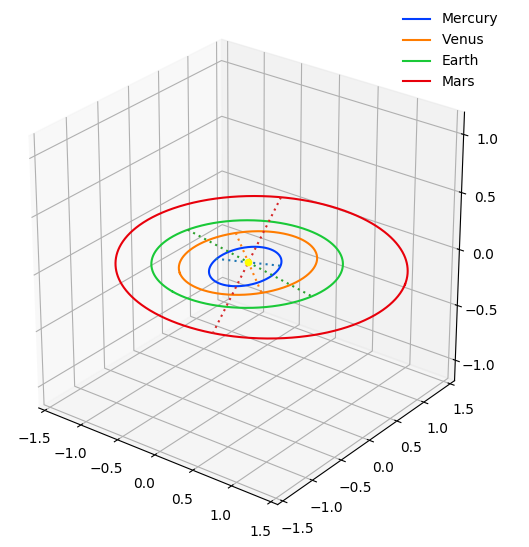
\includegraphics[scale=0.4]{images/plot_example.png}
\caption{Órbitas de Mercurio, Venus, la Tierra y Marte dibujadas con el método \texttt{plotOrbit}.}
\label{fig:plot_example}
\end{figure}


Dado que ya tenemos una estructura para almacenar las coordenadas astronómicas de un objeto y un método que es capaz de representar la elipse definida por dichos elementos, es momento de ponernos a trabajar en la función que nos calcule los elementos orbitales a partir de la posición y velocidad. El código encargado de esta funcionalidad se encontrará en \texttt{scripts/orbital\_elements.py}, y simplemente seguirá los pasos descritos en \ref{sec:elements_determination} para realizar todos los cálculos a partir de la posición y velocidad pasadas como parámetros. Tras hacer los cálculos pertinentes, devolverá un objeto de la clase \texttt{OrbitalObject} con todos los valores obtenidos y como nombre el que se le haya pasado a la función.\\

Así, ya podemos hacer distintas comprobaciones del funcionamiento del código. Nos basta con ir a la efemérides de JPL \cite{jpl}, seleccionar el cuerpo que queramos y anotar su posición y velocidad en un instante $t$. A continuación, utilizamos la función \texttt{getOrbitalElements} pasándole los valores escogidos anteriormente, y podremos dibujar la órbita del objeto que nos devuelva con el método \texttt{plotOrbit}. Un ejemplo de este proceso lo podemos ver en el archivo \texttt{test/test\_1.py}.\\

Una vez explicado el funcionamiento para la representación de datos, pasemos a la parte importante del trabajo, el método de Laplace.\\

\subsection{Implementación del método de Laplace.}
\label{subsec:laplace_method_code}
El desarrollo informático del método de Laplace está basado en una función a la que, pasada una serie de parámetros que contendrán las observaciones de un cuerpo, llamará a una serie de sub-funciones, cada una correspondiente a uno de los pasos vistos en \ref{chap:laplace_method}, y devolverá la posición y velocidad de ese cuerpo en el momento correspondiendo a la segunda observación. Podemos entenderlo mejor con el siguiente pseudocódigo.
\begin{lstlisting}[style=PythonCode]
def Laplace(coordinates, times):
   # Pasamos de ascension recta y declinacion a cartesianas
   position = toCartesian(toRadian(coordinates))
   # Transformamos a dias Julianos
   times = toJulian(times)
   # Calculamos las derivadas (aproximadas)
   EC,EC`,EC`` = approximateDeriv(coordinates,times)
   # Tomamos de la web de JPL el vector Tierra-Sol
   SE,SE`,SE``,R = vectorSE(times[1])
   # Calculamos las distancias $\rho$ y $r$
   rho, r = get_rho_r(EC,EC`,EC``,SE,R)
   # Obtenemos los vectores de posicion y velocidad
   pos, vel = getPosVel(EC,EC`,EC``,SE,SE`,R,r,rho)
   
   Devuelve pos, vel
\end{lstlisting}

Para empezar, tomaremos los valores que se han pasado por parámetro, los cuáles están en ascensión recta y declinación y en formato fecha y hora (año-mes-día hora:minuto), y los pasamos a ecuaciones cartesianas mediante \eqref{eq:equatorial_to_cartesian} y a días julianos \cite{julian}, respectivamente.\\

Continuamos con la función \texttt{approximateDeriv}, que hará exactamente lo que dice su nombre. Utilizando interpolación de Lagrange, se aproximará la primera y segunda derivada del vector $\overrightarrow{EC}$, como hicimos en \ref{sec:series_potencias}.\\

Antes de continuar con el funcionamiento de estas funciones, recordemos las ecuaciones \eqref{eq:relacion_C_S_E}:
\[
\left\{
\begin{array}{l}
	x=\rho\lambda-X\\
	y=\rho\mu-Y\\
	z=\rho\nu-Z
\end{array}
\right.
\]

Tal y como vimos, estas ecuaciones representaban las relaciones entre los tres cuerpos que nos interesan, $C$, $E$ y $S$. Pero para poder resolverlas necesitamos conocer el valor del vector $(X,Y,Z)$. Dado que sería muy cansado tener que tomar la posición (y la velocidad) del Sol de la efemérides cada vez que quisiéramos hacer una aproximación, nos encargaremos de que nuestro programa pueda tomar ese valor automáticamente. Y aquí surge otro problema: no podemos almacenar junto al programa la posición del Sol respecto a la Tierra en todo momento, pues aumentaría el tamaño de este considerablemente. De ahí surge la necesidad de realizar web scraping.\\

\subsubsection{Web Scraping}
La técnica de web scraping es un proceso mediante el cuál podemos obtener información de Internet de manera automatizada. Es una herramienta potente con la que incluso podemos rellenar formularios de manera automática y obtener en formato HTML la página resultante \cite{webscraping}. Para nuestro caso no tendremos que profundizar tanto en las funcionalidades del web scraping, ya que la web de JPL \cite{jpl} nos facilita la obtención de la información del cuerpo que queramos a partir de la URL.\\

De esta manera, definimos en \texttt{util/utilities.py} una función llamada \texttt{getVectorsFromEphemeris} que reutilizaremos a lo largo de la implementación. A dicho método le pasaremos como parámetros los nombres de los cuerpos que $A$ y $B$ que formarán el vector $\overrightarrow{AB}$, el momento en el que queremos tomar el valor del vector y el plano de referencia utilizado (ICRF o eclíptica). Con estos valores formará una \texttt{string} que se corresponderá con la URL que nos devolverá la información requerida. Tras ello, con los paquetes \textit{requests} y \textit{csv} extraeremos la información de la web con dicha URL, a la vez que gestionamos los distintos errores que pueden ocurrir. Finalmente, si todo ha salido bien, se devolverán los vectores de posición y velocidad requeridos y una variable \texttt{True}, y si ha habido algún error, se devolverán vectores de ceros y una variable \texttt{False}.\\

Utilizaremos esta función al llamar al método \texttt{vectorSE}, obteniendo la posición y velocidad del Sol visto desde la Tierra utilizando el plano de referencia ICRF. También se obtendrá el valor de la segunda derivada mediante \eqref{eq:ley_gravitacion_S_E} y la distancia Tierra-Sol, devolviendo finalmente estos cuatro elementos.\\

\subsubsection{Determinación de $\rho$ y $r$ : método de Newton.}
El código desarrollado para determinar $r$ y $\rho$ es el más complejo. Para el cálculo de estos dos valores utilizaremos las secciones \ref{sec:distancias_r_rho} y \ref{sec:newton_rhapson}.\\

La función consistirá en ir calculando los valores de $D$, $D_1$, $N$ y $\psi$ para así llegar a las cantidades $m$ y $M$ de la ecuación \eqref{eq:phi_solution}:
\[
\sin^4{\phi}=M\sin{(\phi+m)}
\]

Una vez tengamos estos valores, iremos utilizando el método de separación de raíces en $[0,\pi]$ para encontrar los subintervalos con una raíz en ellos, y aplicando en su valor intermedio el método de Newton, tal y como vimos en \ref{sec:newton_rhapson}, podremos obtener todas las raíces.
\begin{lstlisting}[style=PythonCode]
def approximate_phi(M,m,tol=1E-09,max_tries=64,plot=False):	
   f = sin(x)^4 - M * sin(x+m)
   
   # Aplicamos el metodo de separacion de raices de Bolzano
   Desde i = 0 hasta max_tries:
      alpha_i = (i*pi) / max_tries
      alpha_{i+1} = ((i+1) * pi) / max_tries
      
      # Si encontramos una raiz en el intervalo ...
      Si signo(f(alpha_i)) != signo(f(alpha_{i+1})):
         # ... tomamos el valor intermedio ...
         x_0 = (alpha_i + alpha_{i+1}) / 2
         
         # ... aplicamos el metodo de Newton ...
         phi, n_iters = newton(f, x_0, tol)
         
         # ... y anyadimos la raiz al resto
         phi_values.anyade(phi)
   
   Si plot:
      dibuja(sin(x)^4)
      dibuja(M * sin(x+m))
      dibuja(phi_values)
   
   Devuelve phi_values
\end{lstlisting}

Además, podremos mostrar si queremos una gráfica por pantalla de la intersección de las funciones junto a las raíces aproximadas, como vemos en el siguiente ejemplo:

\begin{figure}[H]
\centering
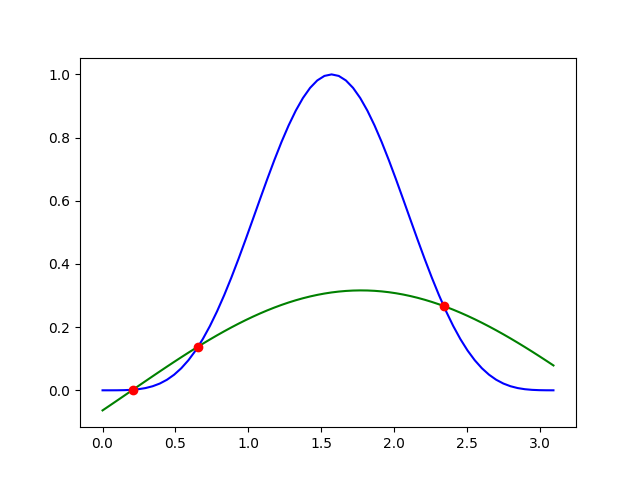
\includegraphics[scale=0.6]{images/example_newton.png}
\caption{Ejemplo de la gráfica que muestra la función \texttt{approximate\_phi} junto a los valores de $\phi$ aproximados.}
\end{figure}

Tras obtener todos los posibles valores de $\phi$ en el intervalo $[0,\pi]$, comprobaremos cuál de ellos es igual a $\pi-\psi$ para discernir entre cuál de los dos restantes es la solución del problema físico, como hicimos en la parte final de \ref{sec:distancias_r_rho}. En el caso de que la solución sea única, se devolverá el valor dicho valor, y si la solución es doble se avisará de ello por pantalla, dando la opción al usuario de elegir entre uno de los dos valores como solución del problema. Se deja para una futura implementación la posibilidad de añadir una cuarta observación para determinar en el caso de una solución doble cuál de las dos es la correcta.\\

Finalmente, con este valor de $\phi$ calcularemos las distancias $r$ y $\rho$ usando \eqref{eq:triangle_relations_2}, y devolveremos estos valores.\\

\subsubsection{Posición y velocidad del cuerpo.}
Una vez hemos obtenido los vectores $\overrightarrow{EC}$ y $\overrightarrow{SE}$ y sus derivadas junto a las distancias $R$, $r$ y $\rho$, solo tendremos que utilizar \eqref{eq:relacion_C_S_E} y \eqref{eq:relacion_C_S_E_derivada} para obtener la posición y velocidad del cuerpo observado.\\

Nótese que los valores obtenidos están respecto al plano ICRF, por lo que una vez que hayamos aplicado por completo el método de Laplace, usaremos la función \texttt{ICRS\_to\_ecliptic} para pasarlos al plano de la eclíptica, tal y como se ha visto en \ref{sec:reference_plane}.\\

\subsection{Estudio del error.}
Para obtener una estimación de cómo de buena ha sido la aproximación del objeto mediante el método de Laplace, se implementarán una serie de funciones para estudiar la diferencia de estas aproximaciones con el valor real.\\

El método \texttt{getApproximationError} tomará como parámetros la posición y velocidad aproximada mediante el método laplaciano de un cuerpo en un instante $t$, así como el nombre del cuerpo que se ha decidido aproximar. Mediante dicho nombre, llamaremos a la función \texttt{getVectorsFromEphemeris} comentada anteriormente para obtener el valor real de la posición y velocidad del cuerpo en el instante $t$ pasado como parámetro. Obtenidos los valores reales, bastará con comprobar la diferencia con los valores aproximados y sus normas, que la función almacenará en una variable \texttt{string}\footnote{Se ha escogido una variable del tipo \texttt{string} para facilitar la impresión por pantalla para la interfaz gráfica.} y devolverá al terminar.\\

\section{Desarrollo de una interfaz gráfica de usuario.}
Todo el código descrito anteriormente es completamente funcional, pero su uso a través de los ficheros en \texttt{tests/} es complicado y poco elegante. Es por ello que nos disponemos a realizar una interfaz gráfica para que la aplicación sea accesible a un mayor número de personas.\\

Como se ha comentado anteriormente, para desarrollar la GUI requerida utilizaremos únicamente el paquete \textit{Tkinter} que viene por defecto en la instalación de Python. La interfaz gráfica implementada se compone básicamente de un formulario en el que introducir los valores de las observaciones y el nombre del cuerpo observado, una serie de botones para realizar distintas funciones con dichos valores y una caja de texto donde mostrar los resultados.

\begin{figure}[H]
\centering
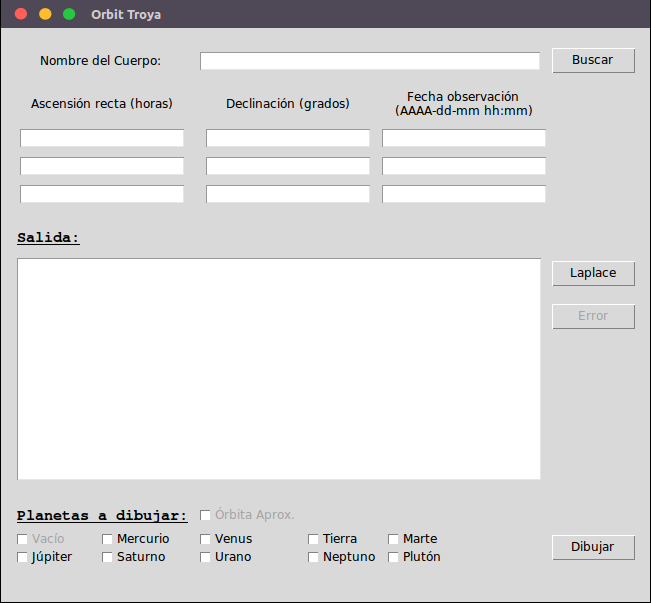
\includegraphics[scale=0.5]{images/gui.png}
\caption{Interfaz gráfica de usuario desarrollada para el método de Laplace.}
\label{fig:gui}
\end{figure}

Para empezar, creamos el directorio \texttt{gui/} que contendrá en su interior un fichero con la definición clase \texttt{OrbitTroya}. En el constructor de esta clase inicializaremos todos los elementos del paquete \textit{Tkinter} que vamos a mostrar en la interfaz y los posicionaremos en el \texttt{grid}.
\begin{itemize}
\item \texttt{Label} para poner los títulos (``Nombre del Cuerpo'', ``Salida:'', etc).
\item \texttt{Entry} para introducir los valores (casillas bajo ascensión recta, declinación y fecha).
\item \texttt{Text} para mostrar los resultados (bajo ``Salida'').
\item \texttt{Checkbutton} para elegir entre los distintos planetas a dibujar (Mercurio, Venus, Tierra, etc).
\item \texttt{Button} para realizar distintas funcionalidades (Buscar, Laplace, Error, Dibujar).
\end{itemize}

Los elementos realmente interesantes para explicar su implementación son los \texttt{Button}, los cuáles contendrán un atributo \texttt{command} y al pulsar sobre ellos llamarán a la función de dicho atributo. Veamos su funcionamiento uno a uno.\\

El botón ``Buscar'' se encargará de tomar el nombre introducido a su izquierda\footnote{Para que funcione correctamente, el nombre debe de ser el oficial proporcionado por el JPL.} y buscar en la efemérides su posición y velocidad respecto al Sol con la función \texttt{getVectorsFromEphemeris} comentada anteriormente. Además, con estos valores calculará las coordenadas astronómicas del objeto buscado. En caso de que se encuentre en la efemérides, se mostrará un mensaje de éxito en el cuadro de texto y se dará la opción de dibujar la órbita de dicho objeto, poniendo el nombre del cuerpo en el \texttt{Checkbutton} ``Vacío'' de la imagen \ref{fig:gui} y haciendo éste botón seleccionable. En caso contrario, se mostrará un mensaje de error en el cuadro de texto y el \texttt{Checkbutton} seguirá igual. Esta funcionalidad está realmente pensada para comparar la órbita real y la aproximada del objeto una vez hayamos aplicado el método de Laplace.\\

Si pulsamos en el botón ``Laplace'', el programa tomará los valores introducidos en el formulario y llamará al método \texttt{Laplace} que vimos en \ref{subsec:laplace_method_code}. Tras ello, pasará las coordenadas de ICRF a la eclíptica, calculará las coordenadas astronómicas, mostrará toda esta información en el cuadro de texto y dará la opción de pinchar en el bóton ``Error''. Finalmente, comprobará si la órbita se puede dibujar (es decir, que $a>0$) y si es así hará seleccionable el \texttt{Checkbutton} ``Órbita Aprox.''.\\

Respecto al botón ``Error'', simplemente tomará los valores de la posición y velocidad aproximados mediante Laplace y mostrará por pantalla el resultado del método \texttt{getApproximationError}.\\

Finalmente, el botón ``Dibujar'' se ocupará de comprobar cuáles de los \texttt{Checkbutton} de su izquierda están seleccionados, añadiéndolos a una lista y llamando al método \texttt{plotOrbit}. Los valores para dibujar los planetas del Sistema Solar estarán almacenados en \texttt{utils/my\_constants.py}.\\

Aunque este programa esté hecho para aplicar el método de Laplace, es curioso que sin darnos cuenta hemos desarrollado un programa capaz de dibujar la órbita de cualquier objeto del Sistema Solar junto a los principales planetas (y Plutón). Bastará con introducir el nombre del cuerpo que queramos dibujar su órbita y darle al botón ``Buscar'', obteniendo de tal manera la posibilidad de dibujar la elipse que forma su movimiento alrededor del Sol.\\

\newpage
\thispagestyle{empty}


\chapter{Experimentación y resultados}
\label{chap:experimentation}
Una vez que hemos desarrollado un software específico para aproximar la órbita de un objeto mediante el método de Laplace, comprobemos su correcto funcionamiento, así como cómo de buenas son los las aproximaciones obtenidas con el método Laplaciano.\\

Dado que no disponemos de instrumental óptimo para realizar las observaciones por nuestra cuenta, utilizaremos (una vez más) la efemérides online del JPL \cite{jpl}, con la que podemos obtener la ascensión recta y declinación observada desde la Tierra de cualquier objeto en cualquier momento. De esta manera, comencemos a ver diferentes resultados prácticos y comentemos la eficacia del método de Laplace que hemos estudiado.\\

\section{Cuando el cuerpo es cercano: Ceres.}
\label{sec:exp_ceres}
Tal y como hemos contado en \label{sec:history}, en 1801 Giuseppe Piazzi descubría el planeta enano Ceres, y meses más tarde Gauss usaba su recientemente desarrollado método para obtener la órbita del objeto con las observaciones que Piazzi había anotado. Gracias a ello, pudieron recuperar la pista de este planeta enano.\\

En ese momento quedó demostrado que el método de Gauss hacía buenas estimaciones para cuerpos a una distancia aproximada a la de Ceres. ¿Hubiera conseguido Laplace unos resultados exitosos? Veámoslo.\\

Vamos a tomar la ascensión recta y declinación de Ceres para ciertos momentos entre los días 28 y 30 de julio de 2020. Los introducimos en el programa desarrollado junto a su nombre, quedando de la siguiente manera:
\begin{figure}[H]
\centering
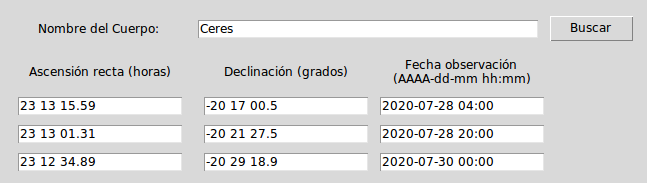
\includegraphics[scale=0.5]{images/ceres_exp.png}
\caption{Datos de Ceres introducidos en el programa.}
\label{fig:ceres_exp}
\end{figure}

Cuando pulsemos el botón ``Buscar'' encontrará en la efemérides el cuerpo requerido de manera satisfactoria.
\begin{lstlisting}[style=Console]
Órbita de Ceres obtenida.
Ahora puedes dibujar el objeto junto al resto.

Nombre = 'Ceres'
a = 2.7672121143653663 UA
e = 0.07772816968324102
i = 10.588147218912999 grados
(*$\Omega$*) = 80.28170111757919 grados
(*$\omega$*) = 73.71539237319364 grados
Período = 1681.3979070284568 días
\end{lstlisting}

A continuación, veamos qué tal funciona el método de Laplace. Con dichos valores, obtenemos los siguientes posibles valores para $\phi$:
\[
\left\{
\begin{array}{l}
\phi_1=11.9311189º\\
\phi_2=37.60583084º\\
\phi_3=134.04867322º
\end{array}
\right.
\]

Dado que $\psi=142.39416916267487º$, cuando calculemos $\pi-\psi$ veremos que es igual a $\phi_2$, por lo que la solución será única y se corresponderá con $\phi_1$.\\

En vez de mostrar el resultado de aplicar el método laplaciano y calcular los elementos orbitales (será más visual compararlo en una gráfica), veamos directamente el error con su valor real utilizando el botón ``Error'':
\begin{lstlisting}[style=Console]
Posición real: [ 2.53436621 -1.48439324 -0.51379219]
Posición calculada: [ 2.54870673 -1.48940124 -0.51764288]
Error = [-0.01434052  0.005008    0.00385069]
|Error| = 0.01567030503509054

Velocidad real: [ 0.00478149  0.00826443 -0.0006202 ]
Velocidad calculada: [ 0.00496131  0.00816816 -0.00068937]
Error = [-1.79816103e-04  9.62781299e-05  6.91715556e-05]
|Error| = 0.0002153787671514888

Distancia real: 2.9816803651312407
Distancia aproximada: 2.9970278967029773
\end{lstlisting}

Podemos observar que la aproximación en $t=$2020-07-28 20:00 es muy buena a pesar de que se haya realizado con tan solo tres observaciones del cuerpo desde la Tierra. Aún así, hay que tener en cuenta que un error en la distancia de $0.01$ UA se corresponde con $1495978.707$ kilómetros.\\

Para terminar, utilicemos las coordenadas astronómicas que hemos aproximado de Ceres para dibujar la órbita asociada a estas coordenadas. Además, añadiremos la órbita real para comprobar cómo de buena es la aproximación, y la órbita de la Tierra para hacernos una pequeña idea de la distancia del cuerpo que hemos utilizado.

\begin{figure}[H]
\centering
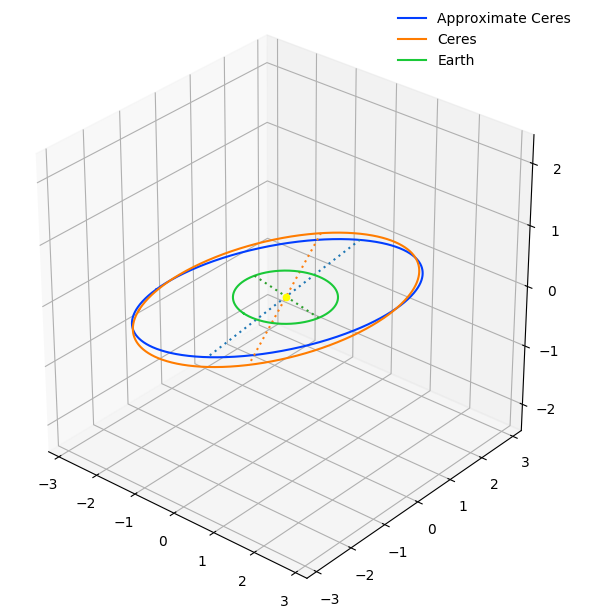
\includegraphics[scale=0.4]{images/plot_ceres.png}
\caption{Órbita real y aproximada de Ceres junto a la Tierra.}
\label{fig:plot_ceres}
\end{figure}

Es fácilmente observable que los elementos orbitales obtenidos a través de la aproximación son muy similares a los reales, y con dicha órbita aproximada podríamos encontrar el planeta enano Ceres en la bóveda celeste. Por tanto, el método de Laplace hubiera sido tan válido como el de Gauss para que en 1801 se hubiese recuperado el cuerpo en el cielo nocturno.\\

\section{El error aumenta con la distancia: Hilda y Plutón.}
\label{sec:exp_hilda_pluton}
Ya hemos visto que con un cuerpo relativamente cercano funciona bien el método de Laplace. Alejémonos un poco más.\\

Empecemos tomando el asteroide Hilda (A875 VC en la efemérides), un objeto que da nombre a un grupo de asteroides situado a unas cuatro unidades astronómicas, entre la órbita de Júpiter y el cinturón de asteroides. Tomamos su ascensión recta y declinación de la efemérides, las introducimos en el programa y aplicamos el método de Laplace.\\

\begin{figure}[H]
\centering
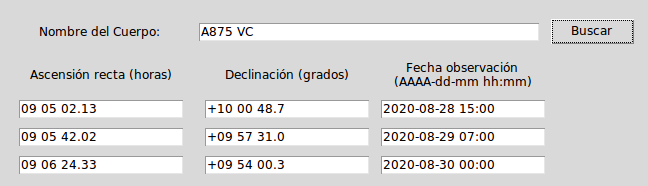
\includegraphics[scale=0.5]{images/hilda_exp.png}
\caption{Datos de Hilda (A875 VC) introducidos en el programa.}
\label{fig:hilda_exp}
\end{figure}

Antes de dar un resultado para la posición y velocidad del cuerpo, el programa para, ya que ha encontrado una solución doble, y nos preguntará sobre cuál de los dos valores posibles queremos tomar como solución del problema físico.\\
\[
\left\{
\begin{array}{l}
\phi_1=4.35491299º\\
\phi_2=18.19187998º\\
\phi_3=158.82202981º=\pi-\psi
\end{array}
\right.
\]

Si escogiésemos $\phi_2$ estaríamos tomando un ángulo mayor al que se encontró como solución en el caso de Ceres, lo cuál no tendría sentido, pues a mayor distancia del cuerpo, menor ángulo forma con la Tierra y el Sol; por tanto, elegiremos como solución $\phi_1$. Nótese que este razonamiento no se podría haber hecho en un caso real de determinación de órbitas, pues a priori no sabemos si el objeto está mas cerca o más lejos con una simple observación.\\

Veamos el resultado que se obtiene tras discernir entre cuál de las dos soluciones es la buena:
\begin{lstlisting}[style=Console]
Aproximación en t = 2020-08-29 07:00:00.000
Posición calculada: [-3.16680643  3.55611002 -0.63839816]
Velocidad calculada: [-6.72694445e-03 -7.39134996e-03 -6.61539321e-05]

Elementos orbitales obtenidos:
Nombre = 'Approximate A875 VC'
a = 12.704405560669025 UA
e = 0.6270295383846635
i = 7.72591356505979 grados
(*$\Omega$*) = 129.50904027965768 grados
(*$\omega$*) = 276.6199742996565 grados
Período = 16540.108377222892 días
\end{lstlisting}

\begin{lstlisting}[style=Console]
Posición real: [-2.83281544  3.23203176 -0.58633104]
Posición calculada: [-3.16680643  3.55611002 -0.63839816]
Error = [ 0.33399099 -0.32407826  0.05206712]
|Error| = 0.46828163075398077

Velocidad real: [-5.32298460e-03 -5.80807100e-03 -1.18918535e-05]
Velocidad calculada: [-6.72694445e-03 -7.39134996e-03 -6.61539321e-05]
Error = [1.40395985e-03 1.58327896e-03 5.42620785e-05]
|Error| = 0.002116794723497365

Distancia real: 4.337586507139335
Distancia aproximada: 4.804386918636096
\end{lstlisting}

Aunque el error en la aproximación de la posición y la velocidad no es excesivamente grande, parece que la cosa no ha ido demasiado bien a la hora de pasar a coordenadas astronómicas, pues habíamos comentado previamente que la distancia del asteroide al Sol era aproximadamente 4 UA, mientras que hemos obtenido una distancia de 12 UA. Veamos una imagen de la órbita calculada junto a la real y las órbitas de la Tierra y Júpiter.

\begin{figure}[H]
\centering
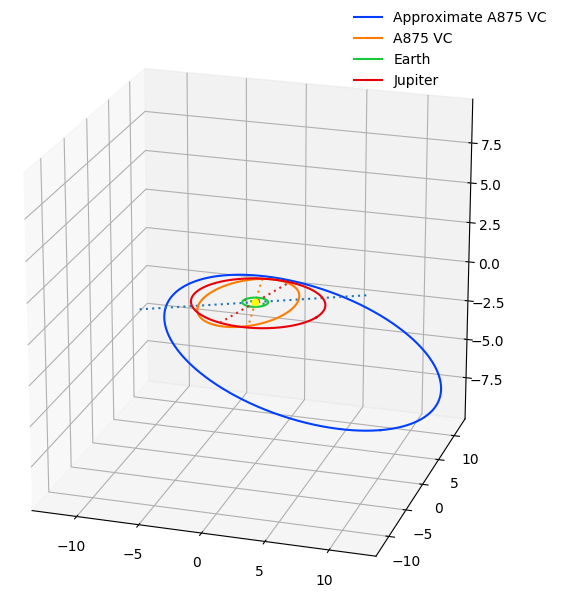
\includegraphics[scale=0.5]{images/hilda_plot.png}
\caption{Órbita real y aproximada de Hilda (A875 VC) junto a la Tierra y Júpiter.}
\label{fig:hilda_plot}
\end{figure}

La aproximación ha sido bastante mala, por lo que no sería mala idea probar con otras observaciones, teniendo en cuenta que podríamos tomarlas más o menos espaciadas que en el caso que hemos estudiado.\\

Comprobemos rápidamente si alejándonos más todavía del Sol sigue aumentando el error de aproximación. Vayámonos muy lejos, concretamente a Plutón. Tomemos sus coordenadas ecuatoriales en tres momentos diferentes y veamos qué tal se porta el método de Laplace.\\

El método se aplica y obtiene una solución de $\phi$ única; en vez de mostrar todo el error, veamos solamente qué tal ha aproximado la distancia al planeta en $t=$2020-09-14 19:00.

\begin{lstlisting}[style=Console]
Posición real: [ 13.74165616 -31.22436196  -0.6327821 ]
Posición calculada: [  7.74035668 -16.5876921   -0.33519062]
Error = [  6.00129948 -14.63666986  -0.29759148]
|Error| = 15.822018227154214
\end{lstlisting}

Con esto podemos ir empezando a sospechar que cuanto mayor sea la distancia al cuerpo observado, mayor será el error que acarrea la aproximación de su posición y velocidad. Es más, el error en esta aproximación hará que al calcular los elementos orbitales obtengamos un semieje mayor negativo, algo que no es posible, y esta aproximación debería ser descartada como solución del problema físico.

\begin{lstlisting}[style=Console]
Aproximación en [...]

Elementos orbitales obtenidos:
Nombre = 'Approximate 999'
a = -0.0019409803348728837 UA
e = 581.0174156903244
[...]

Semieje mayor negativo, no se puede dibujar la órbita.
\end{lstlisting}

\vspace{0.5cm}

\section{Órbitas muy excéntricas: C/2020 F3 (Neowise).}
\label{sec:neowise}
Cuanto mayor sea la excentricidad de un cuerpo espacial, más alejado estarán sus focos, pero más se acercará a ellos en algún momento de su órbita. Este es el caso del objeto C/2020 F3 (Neowise), un cometa del que se oyó mucho hablar durante el pasado mes de julio debido a que, en su trayectoria alrededor del Sol, se acercaba al punto más cercano a la Tierra, de manera que se podía observar a simple vista, y no volvería a ser así hasta dentro de 6765 años.\\

Hemos visto que con objetos muy lejanos la aproximación que nos da el método de Laplace es muy mala. Pero, ¿y si las medidas se toman cuándo el objeto esté muy cercano a la Tierra, de manera que las observaciones sean incluso mejores que las de Ceres?\\

Escogemos los valores de las observaciones del cometa entre el día 14 y el día 15 de julio, en los que su posición en la órbita se encontraba muy cerca de la Tierra.
\begin{figure}[H]
\centering
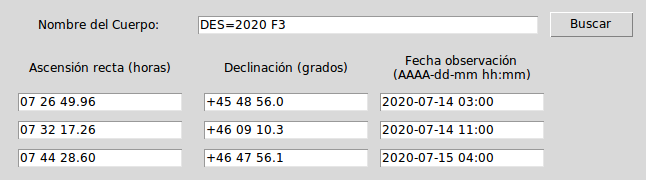
\includegraphics[scale=0.5]{images/neowise_exp.png}
\caption{Datos de C/2020 F3 (Neowise) introducidos en el programa.}
\label{fig:neowise_exp}
\end{figure}

Al aplicar el método de Laplace, volvemos a obtener una solución doble, $\phi_1=90.35678364º$ y $\phi_2=107.33111728º$. En este caso no podemos decidir fácilmente entre cuál de las dos es la válida por lo que elegimos, por ejemplo, $\phi_2$ (y tendremos suerte con la elección). Tras la ejecución, comprobamos el error con la posición y velocidad real en el instante que hemos aproximado.
\begin{lstlisting}[style=Console]
Posición real: [ 0.16652972 -0.24402154  0.32665628]
Posición calculada: [ 0.16854806 -0.25029356  0.32362519]
Error = [-0.00201834  0.00627202  0.00303109]
|Error| = 0.0072525445535108184

Velocidad real: [-0.01084886 -0.03392851  0.00860642]
Velocidad calculada: [-0.0106734  -0.03331783  0.00864502]
Error = [-1.75460689e-04 -6.10680287e-04 -3.85976705e-05]
|Error| = 0.0006365584389714605

Distancia real: 0.44043499684292076
Distancia aproximada: 0.4424800312802405
\end{lstlisting}

Como vemos, los errores al calcular los vectores de posición y velocidad son muy pequeños, hecho que era de esperar al estar tan cerca el objeto que se ha observado. ¿Tendremos la misma suerte con el cálculo de los elementos orbitales?,\\

Comencemos viendo qué tal ha ido la aproximación para la excentricidad y los ángulos $i$, $\Omega$ y $\omega$, comparando los valores en la siguiente tabla.
\begin{table}[H]
\centering
\resizebox{8cm}{!}{%
\begin{tabular}{cc|c}
         & \textit{Valor real}         & \textit{Valor aproximado}   \\ \hline
$e$      & $0.9992401080381621$ & $0.9623385094824053$ \\ \hline
$i$      & $128.9372837890982$  & $129.87582386324678$ \\ \hline
$\Omega$ & $61.01063124644879$  & $60.32375719162504$  \\ \hline
$\omega$ & $37.28105014282296$  & $34.302810750239566$ \\ \hline
\end{tabular}%
}
\end{table}

Parece que todo ha ido bien, por lo que veamos ahora una imagen comparando las dos órbitas.

\begin{figure}[H]
\centering
\subfloat{
	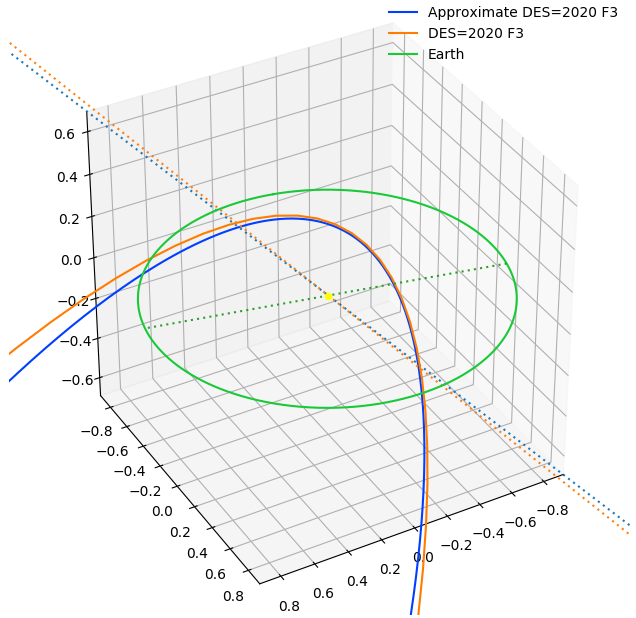
\includegraphics[scale=0.275]{images/neowise_close.png}
	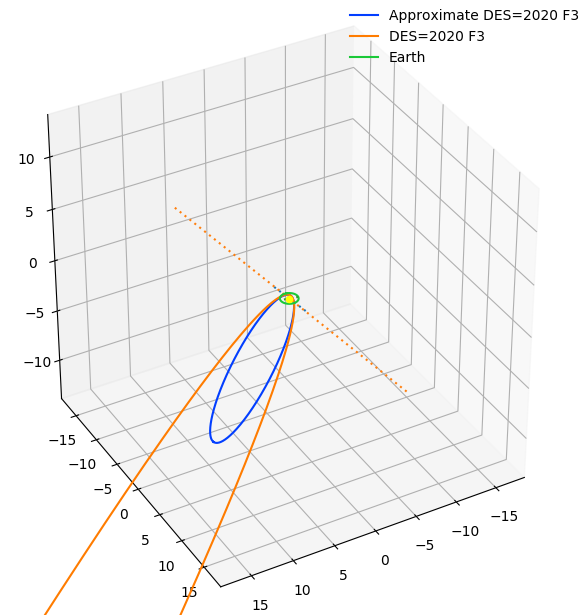
\includegraphics[scale=0.275]{images/neowise_far.png}
}
\caption{Órbita real y aproximada de C/2020 F3 (Neowise) junto a la Tierra vista desde cerca y desde lejos.}
\label{fig:neowise_plot}
\end{figure}

En este caso, observando la órbita de cerca, tenemos una muy buen aproximación, pero conforme nos vamos alejando nos damos cuenta de que ha habido un error muy grande en el semieje mayor: el valor aproximado de $a$ es 7.640204712942875 UA, mientras que el real es de 387.7566248050956 UA, 380 UA de diferencia.\\

Para entender el por qué de este error tan grande tenemos que volver a la sección \ref{sec:elements_determination} y recordar el cálculo de $a$:
\[
h=\frac{|v(t)|^2}{2}-\frac{\mu}{|r(t)|}
\]
\[
a=-\frac{\mu}{2h}
\]

Por tanto, el valor de $a$ depende únicamente del valor de la energía, que se calcula a partir de la norma de la posición y la velocidad. Si tomamos el valor de $a$ como una función en $h$, estaremos ante una función hiperbólica, la cuál divergerá cuando se acerque a 0. Además, para que el valor de $a$ sea muy grande, la energía debe de ser muy cercana a 0. De esta manera, por el hecho de que $a$ diverge en 0, el mínimo error en la energía puede causar un error muy grande en el cálculo del semieje mayor, y esta es la razón del error tan grande obtenido en el semieje mayor del caso de C/2020 F3 (Neowise).


\newpage
\thispagestyle{empty}





\begin{thebibliography}{99}
\bibitem{moulton} \textsc{Moulton, F.R.}, (1914), \textit{An Introduction to Celestial Mechanics}, University of Chicago (USA), Macmillan (second revised edition).

\bibitem{ortega} \textsc{Ortega Ríos, R. \& Ureña Alcázar, A.J.}, (2010), \textit{Introducción a la Mecánica Celeste}, Granada (España), Editorial Universidad de Granada.

\bibitem{mecanica_celeste} \textsc{Ortega Ríos, R.}, \textit{Mecánica Celeste}, Universidad de Granada (España), apuntes del curso 2018-2019.

\bibitem{gronchi} \textsc{Milani, A. \& Gronchi, G.F.}, (2010), \textit{Theory of
orbit determination}, University of Pisa (Italy), Cambridge University Press.

\bibitem{gronchi_unesco} \textsc{Gronchi, G.F.}, Orbit Determination, en \textit{UNESCO Encyclopedia of Life Support Systems, Vol. 6.119.55 Celestial Mechanics}, Eolss Publishers Co Ltd, \href{http://adams.dm.unipi.it/~gronchi/PDF/gronchi_unesco.pdf}{link}.

\bibitem{vetter} \textsc{Vetter, J.R.}, (2007), \textit{Fifty Years of Orbit Determination: Development of Modern Astrodynamics Methods}, Johns Hopkins Apl Technical Digest, \href{https://www.jhuapl.edu/Content/techdigest/pdf/V27-N03/27-03-Vetter.pdf}{link}.

\bibitem{piscis} \textsc{Ridpath, I.}, (2012), \textit{A Dictionary of Astronomy (2 rev. ed.)}, Oxford (UK), Oxford University Press.

\bibitem{right_ascension_declination} \textsc{King, B.}, (2019), \textit{Right Ascension and Declination: Celestial Coordinates For Beginners}, Sky \& Telescope, \href{https://skyandtelescope.org/astronomy-resources/right-ascension-declination-celestial-coordinates/}{link}.

\bibitem{brett_r_wilson} \textsc{Wilson, B.R.}, (2016), \textit{Initial orbit determination through optical observations}, Brigham Young University, Idaho (USA), \href{https://www.byui.edu/documents/physics/Theses/Brett_WilsonS16.pdf}{link} (el archivo se descarga automáticamente).

\bibitem{ASA} \textit{Solution of triangles}, en Wikipedia. Recuperado el 6 de agosto de 2020, \href{https://en.wikipedia.org/wiki/Solution_of_triangles#A_side_and_two_adjacent_angles_given_(ASA)}{link}.

\bibitem{MNII} \textsc{Garralda Guillem, A.I.}, \textit{Métodos Numéricos II}, Universidad de Granada (España), apuntes de clase.

\bibitem{euler_angles} \textsc{Curtis, H.D.}, (2014), \textit{Orbital Mechanics for Engineering Students}, Oxford (United Kingdom), Butterworth-Heinemann (third edition).

\bibitem{ICRF} \textsc{Seidelmann, P.K. \& Kovalevsky, J.}, (2002), \textit{Application of the new concepts and definitions (ICRS, CIP and CEO) in fundamental astronomy}, University of Virginia (USA) \& Observatoire de la Côte d'Azur (France), EDP Sciences, \href{https://www.aanda.org/articles/aa/full/2002/34/aa2452/aa2452.html}{link}.

\bibitem{jpl} \textsc{Park, R.S. (Site Manager) \& Chamberlin A.B. (Webmaster)}, (2020), \textit{HORIZONS Web-Interface} [ephemerides], NASA (USA), \href{https://ssd.jpl.nasa.gov/horizons.cgi}{link}.

\bibitem{geogebra} \textsc{Hohenwarter, M.}, (2001), GeoGebra (6.0.600.0-w) [software]. Obtenido de \href{https://www.geogebra.org/classic}{link}.

\bibitem{numpy} \textsc{Oliphant, T.E. et al.}, (2020), Numpy (1.18.5) and Scipy (1.4.1) [library documentation]. Obtenido de \href{https://docs.scipy.org/doc/}{link}.

\bibitem{matplotlib} \textsc{Hunter, J.D. \& Droettboom, M}, (2020), Matplotlib (3.0.3) [library documentation]. Obtenido de \href{https://matplotlib.org/3.0.3/index.html}{link}.

\bibitem{seaborn} \textsc{Waskom, M.}, (2020), Seaborn (0.9.1) Color Palette [library documentation]. Obtenido de \href{https://seaborn.pydata.org/tutorial/color_palettes.html}{link}.

\bibitem{astropy} \textsc{The Astropy Developers}, (2020) Astropy (3.2.3) [library documentation]. Obtenido de \href{https://docs.astropy.org/en/stable/index.html}{link}.

\bibitem{requests} \textsc{Reitz, K.}, (2020), Requests (2.9.1) [library documentation]. Obtenido de \href{https://requests.readthedocs.io/_/downloads/es/es/latest/pdf/}{link}.

\bibitem{sympy} \textsc{SymPy development team}, (2020), Sympy (1.6.2) [library documentation]. Obtenido de \href{https://docs.sympy.org/latest/index.html}{link}.

\bibitem{tkinter} \textsc{Lundh, F.}, (2020), Tkinter (3.5.1-1) [library documentation]. Obtenido de \href{https://docs.python.org/3/library/tk.html}{link}.

%\bibitem{webscraping} \textsc{Alonso Burgos, S.}, (2020), \textit{"Teoría" de Web Scraping} [Archivo de vídeo]. Recuperado de [vídeo oculto].

\bibitem{webscraping} \textsc{Breuss, M.}, (2019), Beautiful Soup: Build a Web Scraper With Python. Lugar de publicación: \textit{Real Python}, \href{https://realpython.com/beautiful-soup-web-scraper-python/}{link}.

\bibitem{julian} \textsc{Cirillo, J.}, (2015), Día Juliano. Lugar de publicación: \textit{El manual de KStars}, \href{https://docs.kde.org/trunk5/es/extragear-edu/kstars/ai-julianday.html#:~:text=El%20n%C3%BAmero%20de%20d%C3%ADas%20se,n%C3%BAmeros%20de%20sus%20d%C3%ADas%20julianos.}{link}


\end{thebibliography}

\end{document}

